% Escolha: Portugues ou Ingles ou Espanhol.
% Para a versão final do texto, após a defesa, acrescente Final:

\documentclass[Portugues]{phdquali}
%\documentclass[Portugues,Final]{phdquali}

\usepackage[latin1,utf8]{inputenc}

% Usa a fonte Latin Modern
% \usepackage{lmodern}

% Letras gregas (alfa, beta, gamma, etc) em modo texto:
\usepackage{textgreek} % \textalpha, \textbeta, \textgamma, etc

% Para identar primeiro parágrafo:
\usepackage{indentfirst}

% Retira espaço extra obsoleto entre as frases.
\frenchspacing

% Para customizar os gráficos:
\usepackage{float}
\usepackage{graphicx}

% Para transformar caption em negrito:
% \usepackage[font=footnotesize,labelfont=bf]{caption}
\usepackage[font=scriptsize,labelfont=bf]{caption}

% Para citações no formato numérico da norma ABNT:
\usepackage[hyphens]{url}
\usepackage[num,abnt-etal-text=emph,bibjustif]{abntex2cite}
\usepackage{cite}
\renewcommand\citeleft{[}
\renewcommand\citeright{]}

% Para trocar o estilo dos hyperlinks:
\usepackage{hyperref}
\hypersetup{
  colorlinks   = true, % Colours links instead of ugly boxes
  urlcolor     = blue, % Colour for external hyperlinks
  linkcolor    = black, % Colour of internal links
  citecolor   = blue % Colour of citations
}

% Commando para links sem <url>:
% \newcommand{\link}[1]{{\color{blue}\href{#1}{#1}}}

% Para quebrar a linha com urls muito longas:
% \usepackage{breakurl}

% Para usar letras no enumerate:
\usepackage{enumitem}

% Formatar \listoffigures
\usepackage{tocloft}
\renewcommand{\cftfigpresnum}{\bfseries Figura }
\renewcommand{\cftfignumwidth}{6em}
\renewcommand{\cftfigindent}{0em}
\renewcommand{\cfttabpresnum}{\bfseries Tabela }
\renewcommand{\cfttabnumwidth}{6em}
\renewcommand{\cfttabindent}{0em}

% Formatar list of abreviations
\usepackage{acronym}

% Para renderizar formulas matemáticas:
\usepackage{amsmath}
\newcommand{\mAA}{~\text{\AA}}
\newcommand{\aproximadamente}{\raise.2ex\hbox{$\scriptstyle\sim$}}
\newcommand{\less}{\raise.2ex\hbox{$\scriptstyle{<}$}}

% % Para acrescentar comentários ao PDF descomente:
% \usepackage
% %  [pdfauthor={nome do autor},
% %   pdftitle={titulo},
% %   pdfkeywords={palavra-chave, palavra-chave},
% %   pdfproducer={Latex with hyperref},
% %   pdfcreator={pdflatex}]
% {hyperref}

% Define atalhos
\def\ie{i.e.\onedot} 
\def\Ie{I.e.\onedot}
\def\eg{e.g.\onedot}
\def\Eg{E.g.\onedot}

\begin{document}

% Escolha entre autor ou autora:
\autor{João Victor da Silva Guerra}
%\autora{Nome da Autora}

% Sempre deve haver um título em português:
\titulo{Desenvolvimento de plataforma de metodologias computacionais para caracterização estrutural e funcional de biomoléculas e sítios de ligação}

% Se a língua for o inglês ou o espanhol defina:
%\title{The Dissertation or Thesis Title in English or Spanish}

% Escolha entre orientador ou orientadora. Inclua os títulos acadêmicos:
\orientador{Prof. Dr. Paulo Sergio Lopes-de-Oliveira}
%\orientadora{Profa. Dra. Nome da Orientadora}

% Escolha entre coorientador ou coorientadora, se houver.  Inclua os títulos acadêmicos:
%\coorientador{Prof. Dr. Eng. Lic. Nome do Co-Orientador}
%\coorientadora{Profa. Dra. Eng. Lic. Nome da Co-Orientadora}

% Escolha entre mestrado ou doutorado:
% \mestrado
\doutorado

% Se houve cotutela, defina:
%\cotutela{Universidade Nova de Plutão}

\datadadefesa{29}{08}{2023}

% Para a versão final defina:
%\avaliadorA{Prof. Dr. Primeiro Avaliador}{Instituição do primeiro avaliador}
%\avaliadorB{Profa. Dra. Segunda Avaliadora}{Instituição da segunda avaliadora}
%\avaliadorC{Dr. Terceiro Avaliador}{Instituição do terceiro avaliador}
%\avaliadorD{Prof. Dr. Quarto Avaliador}{Instituição do quarto avaliador}
%\avaliadorE{Prof. Dr. Quinto Avaliador}{Instituição do quinto avaliador}
%\avaliadorF{Prof. Dr. Sexto Avaliador}{Instituição do sexto avaliador}
%\avaliadorG{Prof. Dr. Sétimo Avaliador}{Instituição do sétimo avaliador}
%\avaliadorH{Prof. Dr. Oitavo Avaliador}{Instituição do oitavo avaliador}


% Para incluir a ficha catalográfica em PDF na versão final, descomente e ajuste:
%\fichacatalografica{arquivo.pdf}


% Este comando deve ficar aqui:
\paginasiniciais


% Se houver dedicatória, descomente:
%A dedicatória deve ocupar uma única página.
% \prefacesection{Dedicatória}
% Este trabalho de pesquisa é dedicado a você, familiar ou amigo que contribuiu muito na minha caminhada. Sem vocês eu nada teria.

% Se houver epígrafe, descomente e edite:
\begin{epigrafe}
{
  Sem dados você é apenas mais uma pessoa com uma opinião.
}
\hfill (William E. Deming)
\end{epigrafe}

% Agradecimentos ou Acknowledgements ou Agradecimientos
\prefacesection{Agradecimentos}

Gostaria de expressar meus sinceros agradecimentos a todos que me apoiaram durante o desenvolvimento deste projeto. Em primeiro lugar, sou grato aos meus pais, Roseli do Carmo Freitas da Silva e Mario Luiz da Silva Guerra, por me apoiarem em todas as etapas da minha formação acadêmica e profissional. Agradeço à minha companheira, Bruna Martins da Silva, pelo apoio incondicional em todas as fases deste projeto.

Gostaria de agradecer ao meu orientador, Dr. Paulo Sergio Lopes de Oliveira, por ter me dado liberdade científica e criativa para desenvolver esta tese e, acima de tudo, pela oportunidade de trabalhar em um centro de pesquisa de excelência com um suporte essencial de sua parte. Agradeço aos meus colegas do Laboratório de Biologia Computacional, Dr. José Geraldo de Carvalho Pereira, Dr. Helder Veras Ribeiro Filho, MSc. Luiz Fernando Giolo Alves, Dra. Mariana Bortoletto Grizante, Dr. Gabriel Ernesto Jara e Dr. Leandro Oliveira Bortot, por me apoiarem em momentos importantes, compartilhando ideias e sugestões para o desenvolvimento deste projeto. Especificamente, gostaria de agradecer ao apoio no desenvolvimento e planejamento das ferramentas ao Dr. Helder Veras Ribeiro Filho e do Dr. José Geraldo de Carvalho Pereira, além do suporte em temas relacionados à dinâmica molecular fornecido pelo Dr. Gabriel Ernesto Jara e pelo Dr. Leandro Oliveira Bortot. Sou imensamente grato a todos que me ajudaram nesta etapa essencial da minha formação acadêmica.

Por fim, gostaria de agradecer ao Programa de Pós-Graduação em Ciências Farmacêuticas (PPGCF) da Faculdade de Ciências Farmacêuticas (FCF) da Universidade Estadual de Campinas (UNICAMP), ao Laboratório Nacional de Biociências (LNBio) e ao Centro Nacional de Pesquisa em Energia e Materiais (CNPEM), por terem viabilizado este trabalho. Também sou grato pelo apoio financeiro da Fundação de Amparo à Pesquisa do Estado de São Paulo (FAPESP) pelo projeto de pesquisa regular (processo nº 2018/00629-0).

% Sempre deve haver um resumo em português.
% O resumo deve ter no máximo 500 palavras e deve ocupar uma única página.
\begin{resumo}

Nos últimos tempos, temos testemunhado o avanço das aplicações de ciência de dados e inteligência artificial (IA) em diversas áreas do conhecimento. Desde o processamento de linguagem natural com o ChatGPT até a biologia estrutural com o AlphaFold, tecnologias de IA têm transformado a forma como abordamos e compreendemos problemas complexos. No campo das interações biomoleculares, o estudo das biomoléculas e seus sítios de ligação é fundamental para compreender os processos biológicos e aprimorar o desenvolvimento de novos fármacos. No entanto, investigar os mecanismos intrínsecos dessas interações ou identificar possíveis locais de interação ainda é um desafio devido à complexidade das biomoléculas e à diversidade das interações que ocorrem entre elas. 

Diante desse cenário, a demanda por ferramentas computacionais robustas e abrangentes para estudos de sistemas biomoleculares tem crescido. É nesse contexto que introduzimos o KVFinder suite, uma plataforma computacional desenvolvida para atender a essas necessidades. O KVFinder suite é composto por um conjunto de ferramentas que englobam a codificação e caracterização de biomoléculas e seus sítios de ligação, a saber: parKVFinder, pyKVFinder, KVFinder-web, SERD e KVFinderMD, o conjunto oferece uma variedade de funcionalidades que visam suprir as demandas da comunidade de biologia estrutural. Cada uma das ferramentas desempenha um papel específico dentro do KVFinder suite. Elas permitem a codificação de informações estruturais e características relevantes dos sítios de ligação, além de possibilitar a análise e a caracterização dessas informações e até mesmo o uso de suas unidades básicas para aplicações de ciências de dados e IA. Ao longo deste trabalho, foram apresentadas aplicações bem-sucedidas das ferramentas do KVFinder suite em estudos de caso de interesse terapêutico, que evidenciam a sua eficácia, bem como novas implementações de caracterizações biomoleculares, fornecendo uma referência valiosa para a comunidade científica construir suas próprias aplicações.

A plataforma KVFinder suite apresenta um avanço significativo no campo da biologia computacional estrutural, oferecendo um conjunto abrangente de ferramentas para a análise e caracterização de biomoléculas e seus sítios de ligação. Com sua diversidade de funcionalidades e a capacidade de se integrar em aplicações de ciência de dados e/ou IA, o KVFinder suite tem o potencial de impulsionar avanços na compreensão dos mecanismos de interação biomolecular e no desenvolvimento de novas estratégias terapêuticas. A disponibilidade dessa plataforma para a comunidade científica representa um importante recurso que contribuirá para a aceleração da pesquisa e o avanço do conhecimento na área.

\end{resumo}

% Sempre deve haver um abstract.
% The abstract must have at most 500 words and must fit in a single page.
\begin{abstract}

Nowadays, we have witnessed the advancement of data science and artificial intelligence applications in various fields of knowledge. From natural language processing with ChatGPT to structural biology with AlphaFold, these technologies have transformed the way we approach and understand complex problems. In the field of biomolecular interactions, the study of biomolecules and their binding sites is crucial for understanding biological processes and improving the development of new drugs. However, investigating the intrinsic mechanisms of these interactions or identifying potential interaction sites is still challenging due to the complexity of biomolecules and the diversity of interactions that occur among them.

Given this situation, the demand for robust and comprehensive computational tools for studying biomolecular systems has been growing. In this context, we introduce the KVFinder suite, a computational platform developed to meet these needs. The KVFinder suite consists of a set of tools that encompass the encoding and characterization of biomolecules and their binding sites. Comprising the tools parKVFinder, pyKVFinder, KVFinder-web, SERD, and KVFinderMD, the suite offers a variety of functionalities aimed at addressing the demands of the structural biology community. Each of these tools plays a specific role within the KVFinder suite. They allow for the encoding of structural information and relevant features of binding sites, as well as enable the analysis and characterization of this information, and even the utilization of their basic units for data science and artificial intelligence applications. Throughout this work, successful applications of the KVFinder suite tools in therapeutic case studies have been presented, demonstrating their effectiveness, as well as new implementations of characterizations, providing a reference for the scientific community to build their own applications.

The KVFinder suite platform represents a significant advancement in the field of structural biology, offering a comprehensive set of computational tools for the analysis and characterization of biomolecules and their binding sites. With its diverse functionalities and the ability to integrate with data science and artificial intelligence applications, the KVFinder suite has the potential to drive advances in the understanding of biomolecular interaction mechanisms and the development of new therapeutic strategies. The availability of this platform to the scientific community represents an important resource that will contribute to accelerating research and advancing knowledge in the field.

\end{abstract}


% Se houver um resumo em espanhol, descomente:
%\begin{resumen}
% A mesma regra aplica-se.
%\end{resumen}


% A lista de figuras é opcional:
\listoffigures
\clearpage

% A lista de tabelas é opcional:
% \listoftables
% \clearpage

% A lista de abreviações e siglas é opcional:
\prefacesection{Lista de Abreviações e Siglas}

\begin{acronym}
  \acro{3D}{Tridimensional}
  \acro{ADRP}{\textit{ADP-ribose phosphatase}}
  \acro{API}{\textit{Application Programming Interface}}
  \acro{CHIKV}{\textit{Chikungunya virus}}
  \acro{CLI}{\textit{command-line interface}}
  \acro{CNPEM}{Centro Nacional de Pesquisa em Energia e Materiais}
  \acro{DFS}{\textit{Depth-First Search}}
  \acro{DM}{Dinâmica molecular}
  \acro{EEEV}{\textit{Eastern Equine Encephalitis virus}}
  \acro{FAPESP}{Fundação de Amparo à Pesquisa do Estado de São Paulo}
  \acro{FCF}{Faculdade de Ciências Farmacêuticas}
  \acro{GHECOM}{\textit{Grid-based HECOMi finder}}
  \acro{GUI}{\textit{Graphical User Interface}}
  \acro{HIV-1}{\textit{Human Immunodeficiency Virus type 1}}
  \acro{HTTP}{\textit{HyperText Transfer Protocol}}
  \acro{IA}{Inteligência Artificial}
  \acro{IPD}{Interações Proteína-DNA}
  \acro{IPL}{Interações Proteína-Ligante}
  \acro{IPR}{Interações Proteína-RNA}
  \acro{IPP}{Interações Proteína-Proteína}
  \acro{IV CEC}{IV Congresso de Estudantes do CNPEM}
  \acro{KVFinderMD}{\textit{KVFinder for Molecular Dynamics analysis}}
  \acro{LBC}{Laboratório de Biologia Computacional}
  \acro{LES}{Superfície Excluída pelo Ligante (\textit{Ligand Excluded Surface})}
  \acro{LNBio}{Laboratório Nacional de Biociências}
  \acro{MAYV}{\textit{Mayaro virus}}
  \acro{ndarray}{\textit{N-dimensional array}}
  \acro{Nsps}{\textit{Non-structural proteins}}
  \acro{parKVFinder}{\textit{Parallel KVFinder}}
  \acro{PDB}{\textit{Protein Data Bank}}
  \acro{Pi}{\textit{Probe In}}
  \acro{Po}{\textit{Probe Out}}
  \acro{PPGCF}{Programa de Pós-Graduação em Ciências Farmacêuticas}
  \acro{pyKVFinder}{\textit{Python-C Parallel KVFinder}}
  \acro{RMSD}{\textit{Root-Mean-Square Deviation}}
  \acro{SARS-CoV-2}{\textit{Severe acute respiratory syndrome Coronavirus 2}}
  \acro{SAS}{Superfície Acessível ao Solvente (\textit{Solvent Accessible Surface})}
  \acro{SES}{Superfície Excluída pelo Solvente (\textit{Solvent Excluded Surface})}
  \acro{SINV}{\textit{Sindbis virus}}
  \acro{UNICAMP}{Universidade Estadual de Campinas}
  \acro{vdW}{van der Waals}
  \acro{VEEV}{\textit{Venezuelan Equine Encephalitis virus}}
  \acro{wwPDB}{Worldwide Protein Data Bank}
\end{acronym}

\clearpage

% A lista de símbolos é opcional:
% \prefacesection{Lista de Símbolos}

% Quem usa o pacote nomencl pode incluir:
% \renewcommand{\nomname}{Lista de Abreviações e Siglas}
% \printnomenclature[3cm]

% O sumário vem aqui:
\tableofcontents

% E esta linha deve ficar bem aqui:
\fimdaspaginasiniciais

% O corpo da dissertação ou tese começa aqui:

%%% Chapter 1

\chapter{Introdução}

Biomoléculas, como proteínas e ácidos nucleios, são moléculas complexas que desempenham funções biológicas essenciais para a vida. Processos biológicos, como a transdução de sinal, a integridade estrutural, a adesão celular e a apoptose, são modulados por interações biomoleculares \cite{sotriffer2002,henrich2010}. Essas interações são extremamente importantes para a compreensão de processo biológicos e para o desenvolvimento e/ou aprimoramento de terapias farmacológicas \cite{henrich2010}. No entanto, os estudos dos mecanismos intrínsicos dessas interações ou possíveis pontos de interação são desafiadores, devido à complexidade das biomoléculas e à diversidade das interações que ocorrem entre elas.

Usualmente, essas interações ocorrem entre os receptores e ligantes, que variam de íons, como ferro e fosfato, a macromoléculas, como proteínas, RNA e DNA \cite{oliveira2014}. Para execução dessas interações, estruturas moleculares se dobram orquestradamente para criar sítios de ligação específicos, comumente localizados em cavidades ao longo da superfície molecular, expondo padrões topológicos e físico-químicos para acomodar ligantes específicos \cite{henrich2010,guerra2021}. As interações receptor-ligante, como interações proteína-proteína (IPP), proteína-ligante (IPL), proteína-RNA (IPR) e proteína-DNA (IPD), são consequência da complementariedade entre as superfícies moleculares do par de interação, restringindo assim a um pequeno número de ligantes a interação eficiente com um dado receptor \cite{henrich2010,simoes2017}.

Dada a importância das interações biomoleculares, o estudo das biomoléculas e seus sítios de ligação é essencial para compreensão de processos biológicos e para o aprimoramento e desenvolvimento de novos fármacos. A utilização de abordagens computacionais para identificar sítios de ligação e caracterizar interações biomoleculares tem se mostrado uma alternativa eficaz para complementar os métodos experimentais e fornecer informações detalhadas sobre as interações moleculares \cite{simoes2017}. A identificação de sítios de ligação é um problema de classificação, onde o objetivo é determinar se um dado ponto na superfície de uma biomolécula é um sítio de ligação ou não \cite{sotriffer2002,henrich2010,simoes2017}. Enquanto isso, avanços em recursos computacionais e base de dados têm impulsionado o uso de métodos \textit{in silico} para simular a dinâmica de biomoléculas e implementar aplicações de IA para estudar estruturas biomoleculares \cite{tunyasuvunakool2021}. Juntos, todos esses dados estruturais fornecem terreno fértil para interpretação de dados por meio de ciência de dados ou protocolos automatizados, mas a análise intensiva de dados requer rotinas eficientes e integráveis com uma estrutura de dados facilmente manipulável.

Nesse cenário, ainda há a necessidade de ferramentas computacionais robustas e abrangentes para estudos computacionais de sistemas biomoleculares, capazes de cobrir as diferentes formas de interação. Ferramentas que sirvam como blocos de construção, para aplicações, programas e/ou protocolos automatizados de biologia computacional, biologia estrutural, aprendizado de máquina e áreas correlatas, são essenciais para análise de biomoléculas e/ou sítios de ligação. O desenvolvimento de ferramentas que possam ser utilizadas em diferentes tipos de aplicações e potencialidades é de suma importância nesse contexto.

Nesse sentido, o KVFinder suite é uma plataforma computacional que tem como objetivo atender a essas demandas. O KVFinder suite é composto por um conjunto de ferramentas para codificação e caracterização de biomoléculas e detecção e caracterização de sítios de ligação nessas biomoléculas. O KVFinder suite é composto por cinco ferramentas: parKVFinder \cite{guerra2020}, pyKVFinder \cite{guerra2021}, KVFinder-web \cite{guerra2023A}, SERD e KVFinderMD. Essa plataforma tem o potencial de ser uma ferramenta robusta e abrangente para estudos computacionais de sistemas biomoleculares, e pode ser utilizada em diferentes aplicações e contextos, desde a biologia estrutural até a ciência de dados.

\section{Identificação de sítios de ligação em biomoléculas \label{sec:binding-sites}}

Ao longo das últimas décadas, diversas abordagens \textit{in silico} foram desenvolvidas para identificação de sítios de ligação em proteínas para aprofundar os conhecimentos acerca da função de uma determinada proteína e para descoberta e melhoramento de fármacos \cite{liang1998}. No entanto, apenas algumas metodologias são aplicáveis a outros tipos de biomoléculas, \eg, ácidos núcleicos, carboidratos e lípideos. As abordagens computacionais publicadas podem ser divididas em três categorias principais: geométricas, energéticas e evolutivas \cite{oliveira2014,simoes2017}.

\begin{itemize}
  \item \textbf{Métodos evolutivos:} são baseados na busca por resíduos conservados em alinhamentos de sequências múltiplas e informações de perfis conhecidos de sítios de ligação;
  \item \textbf{Métodos energéticos:} identificam sítios de ligação a partir da interação energética entre a biomolécula-alvo e uma sonda química, geralmente um grupo químico;
  \item \textbf{Métodos geométricos:} identificam cavidades analisando as características geométricas da superfície molecular.
\end{itemize}

Cada categoria de métodos possui suas próprias vantagens e desvantagens \cite{sotriffer2002,henrich2010,simoes2017,krone2016}. Algoritmos evolutivos dependem fortemente de informações de sequência ou bancos de dados de sítios de ligação ativos e da qualidade do procedimento de alinhamento, enquanto os métodos energéticos dependem de procedimentos de filtragem, parametrizações de campo de força e funções de pontuação utilizadas. Por outro lado, métodos de detecção geométrica são relativamente simples e diretos e não exigem nenhum conhecimento não geométrico, apenas dados estruturais da proteína, \ie, o arquivo no formato \textit{Protein Data Bank} (PDB), XYZ, mmCIF ou equivalente, contendo as coordenadas cartesianas dos átomos, que podem ser facilmente acessadas no Worldwide Protein Data Bank (wwPDB). Uma vez que as coordenadas dos átomos estão disponíveis, métodos geométricos devem ser capazes de representar qualquer tipo de biomolécula \cite{henrich2010,oliveira2014,simoes2017}. Embora métodos puramente geométricos sejam eficientes na identificação de todos os tipos de cavidades de uma molécula alvo, identificar aquelas que são funcionalmente relevantes apresenta um problema. No entanto, a caracterização de cavidades em termos de propriedades físico-químicas bem escolhidas pode levar à identificação de cavidades funcionalmente relevantes, ou seja, sítios de ligação para um conjunto específico de ligantes \cite{sotriffer2002,henrich2010,simoes2017,liang1998}.

Geralmente, algoritmos baseados em geometria são os mais frequentemente usados para detectar cavidades em proteínas. Enquanto métodos baseados em evolução seriam limitados a proteínas porque dependem de princípios da evolução biológica, métodos baseados em energia poderiam ser aplicáveis, mas exigiriam ajustes finos dos parâmetros de campo de força adaptados à outros tipos de biomoléculas. Como ácidos nucleicos, carboidratos e lipídeos podem ter propriedades distintas em comparação com proteínas, métodos que dependem apenas de informações geométricas (por exemplo, coordenadas Cartesianas tridimensionais (3D) e tamanho do átomo) são desejáveis.

\subsection{Abordagens geométricas \label{sec:geometric-approaches}}

A detecção de cavidades através de abordagens geométricas é amplamente utilizada, envolvendo diferentes técnicas \cite{simoes2017,guerra2020,krone2016}. Essas técnicas são simples, diretas e não requerem conhecimento prévio, tornando-as as mais comumente utilizadas na literatura \cite{henrich2010,oliveira2014}. Neste contexto, apresentamos uma breve classificação das abordagens geométricas para detecção de cavidades, incluindo técnicas baseadas em grade 3D, sonda, tesselação, superfície e suas combinações \cite{simoes2017,guerra2020,krone2016,guerra2023B}.

\begin{itemize}
  \item \textbf{Algoritmos baseados em grade 3D} (\eg, POVME 3.0 \cite{povme}) representam um conjunto de átomos como pontos discretos, geralmente usando uma grade 3D alinhada aos eixos, como um campo escalar, ou seja, um mapa de densidade, onde cada ponto discreto é um valor inteiro ou booleano. Esses mapas de grade são usados para agrupar pontos de espaço vazio relevantes (\ie, não pertencentes ao soluto) em cavidades usando algoritmos de agrupamento de voxels. Normalmente, esses métodos utilizam estruturas de dados simples, capazes de representar uma coleção de dados em um ponto discreto e identificar cavidades de forma automatizada. No entanto, a precisão geométrica, o tempo de computação e o consumo de memória dependem fortemente da resolução da grade, ou seja, da sensibilidade ao espaçamento da grade. Além disso, esses métodos não são invariantes à rotação, o que significa que a orientação de uma determinada molécula afeta ligeiramente a precisão, ou seja, a sensibilidade à orientação;

  \item \textbf{Algoritmos baseados em sondas} (\eg, pywindow \cite{pywindow}, PHECOM \cite{phecom}) utilizam um conjunto de átomos, considerando suas coordenadas 3D e raios de van der Waals, para representar a superfície molecular, que é analisada por uma ou mais sondas, geralmente esferas rígidas, para investigar seus níveis de acessibilidade. Essa técnica pode detectar qualquer tipo de cavidade e está relacionada à extensão espacial de ligantes em potencial; no entanto, pode ter dificuldades em encontrar e delinear de forma inequívoca os limites entre a cavidade e o solvente, ou seja, a ambiguidade na abertura da boca;
  
  \item \textbf{Algoritmos baseados em tesselação} (\eg, Fpocket \cite{fpocket}, CAVER 3.0 \cite{caver3}) dependem de técnicas de geometria computacional, como formas \textalpha, formas \textbeta, diagramas de Voronoi e diagramas de Apollonius. Especificamente, formas \textalpha\space e tesselação de Voronoi usam centros atômicos, esferas implicitamente de raio constante para modelar átomos, enquanto formas \textbeta\space e métodos baseados em Apollonius dependem de esferas de raio variável para modelar esses átomos, que são explorados para identificar cavidades. Normalmente, esses métodos não dependem de nenhuma informação da superfície molecular para detectar cavidades, mas podem ter dificuldades em identificar a localização correta do sítio de ligação, identificar e delinear os limites entre a cavidade e o solvente e definir o número de átomos de superfície;

  \item \textbf{Algoritmos baseados em superfície} (\eg, NSA \cite{nsa}, MSPocket \cite{mspocket}) não utilizam um modelo de esfera rígida, mas sim um modelo de superfície molecular, como a superfície de van der Waals (vdW), superfície excluída pelo solvente (\textit{Solvent Excluded Surface}; SES), superfície acessível ao solvente (\textit{Solvent Accessible Surface}; SAS) e a superfície excluída pelo ligante (\textit{Ligand Excluded Surface}; LES), que define a interface molecular e seu ambiente. A análise da interface molecular identifica cavidades com base na acessibilidade a um solvente específico ou a um ligante. Nesse caso, a detecção de cavidades ocorre de maneira automatizada, assim como nos métodos baseados em grade, porém não apresenta a ambiguidade na abertura da boca. No entanto, em alguns casos, esses algoritmos podem ter dificuldades em detectar todos os tipos de cavidades e sua extensão completa.
\end{itemize}

Geralmente, a combinação dessas técnicas (\eg, parKVFinder \cite{guerra2020}, pyKVFinder \cite{guerra2021}, KVFinder-web \cite{guerra2023B}, GHECOM \cite{ghecom}, MoloVol \cite{molovol}) tem como objetivo aproveitar as capacidades de cada uma e corrigir ou mitigar suas deficiências individuais, a fim de obter uma técnica mais robusta, como os métodos baseados em grade e esfera, que não são sensíveis à orientação como os métodos baseados em grade. Portanto, cada técnica possui suas próprias capacidades e deficiências, o que torna cada método mais adequado para determinadas aplicações \cite{simoes2017,krone2016}.

\subsection{Principais ferramentas disponíveis para detecção e caracterização de sítios de ligação}

A grande maioria dos ferramentas de detecção de cavidades foi originalmente desenvolvida para proteínas (veja a Seção \ref{sec:geometric-approaches}). Embora esses algoritmos sejam robustos o suficiente para descrever e analisar qualquer sistema de moléculas (\eg, proteína, DNA, RNA, materiais inorgânico, gaiola supramolecular, etc), até o momento, apenas algumas poucas ferramentas foram aplicadas à outros sistemas biomoleculares, que não incluem proteínas, para avaliar características estruturais, como forma e volume de suas cavidades e aberturas. 

Nesse cenário, revisamos cuidadosamente à literatura para selecionar ferramentas de detecção capazes de estudar qualquer sistema molecular, gratuitos, bem documentados, com suporte adequado pelos desenvolvedores e reconhecidos na comunidade científica. Com base nesses critérios, descrevemos as quatro principais ferramentas de detecção de cavidades identificadas. A seguir, uma breve descrição de seus algoritmos e funcionalidades.

\subsubsection{KVFinder suite}

O KVFinder suite é uma plataforma abrangente de ferramentas para a codificação e caracterização de biomoléculas, bem como a detecção e caracterização de sítios de ligação nessas biomoléculas. Na plataforma, o algoritmo de detecção de cavidades (Figura \ref{fig:kvfinder-suite-schema}) utiliza uma metodologia de dupla sonda baseado na teoria de morfologia matemática, originalmente implementado na ferramenta KVFinder \cite{oliveira2014}. Nesse método, uma sonda menor (\textit{Probe In}) e uma sonda maior (\textit{Probe Out}) inspecionam os pontos da grade, definindo as cavidades como as regiões não sobrepostas percorridas por essas sondas. 

\begin{figure}[ht]
  \centerline{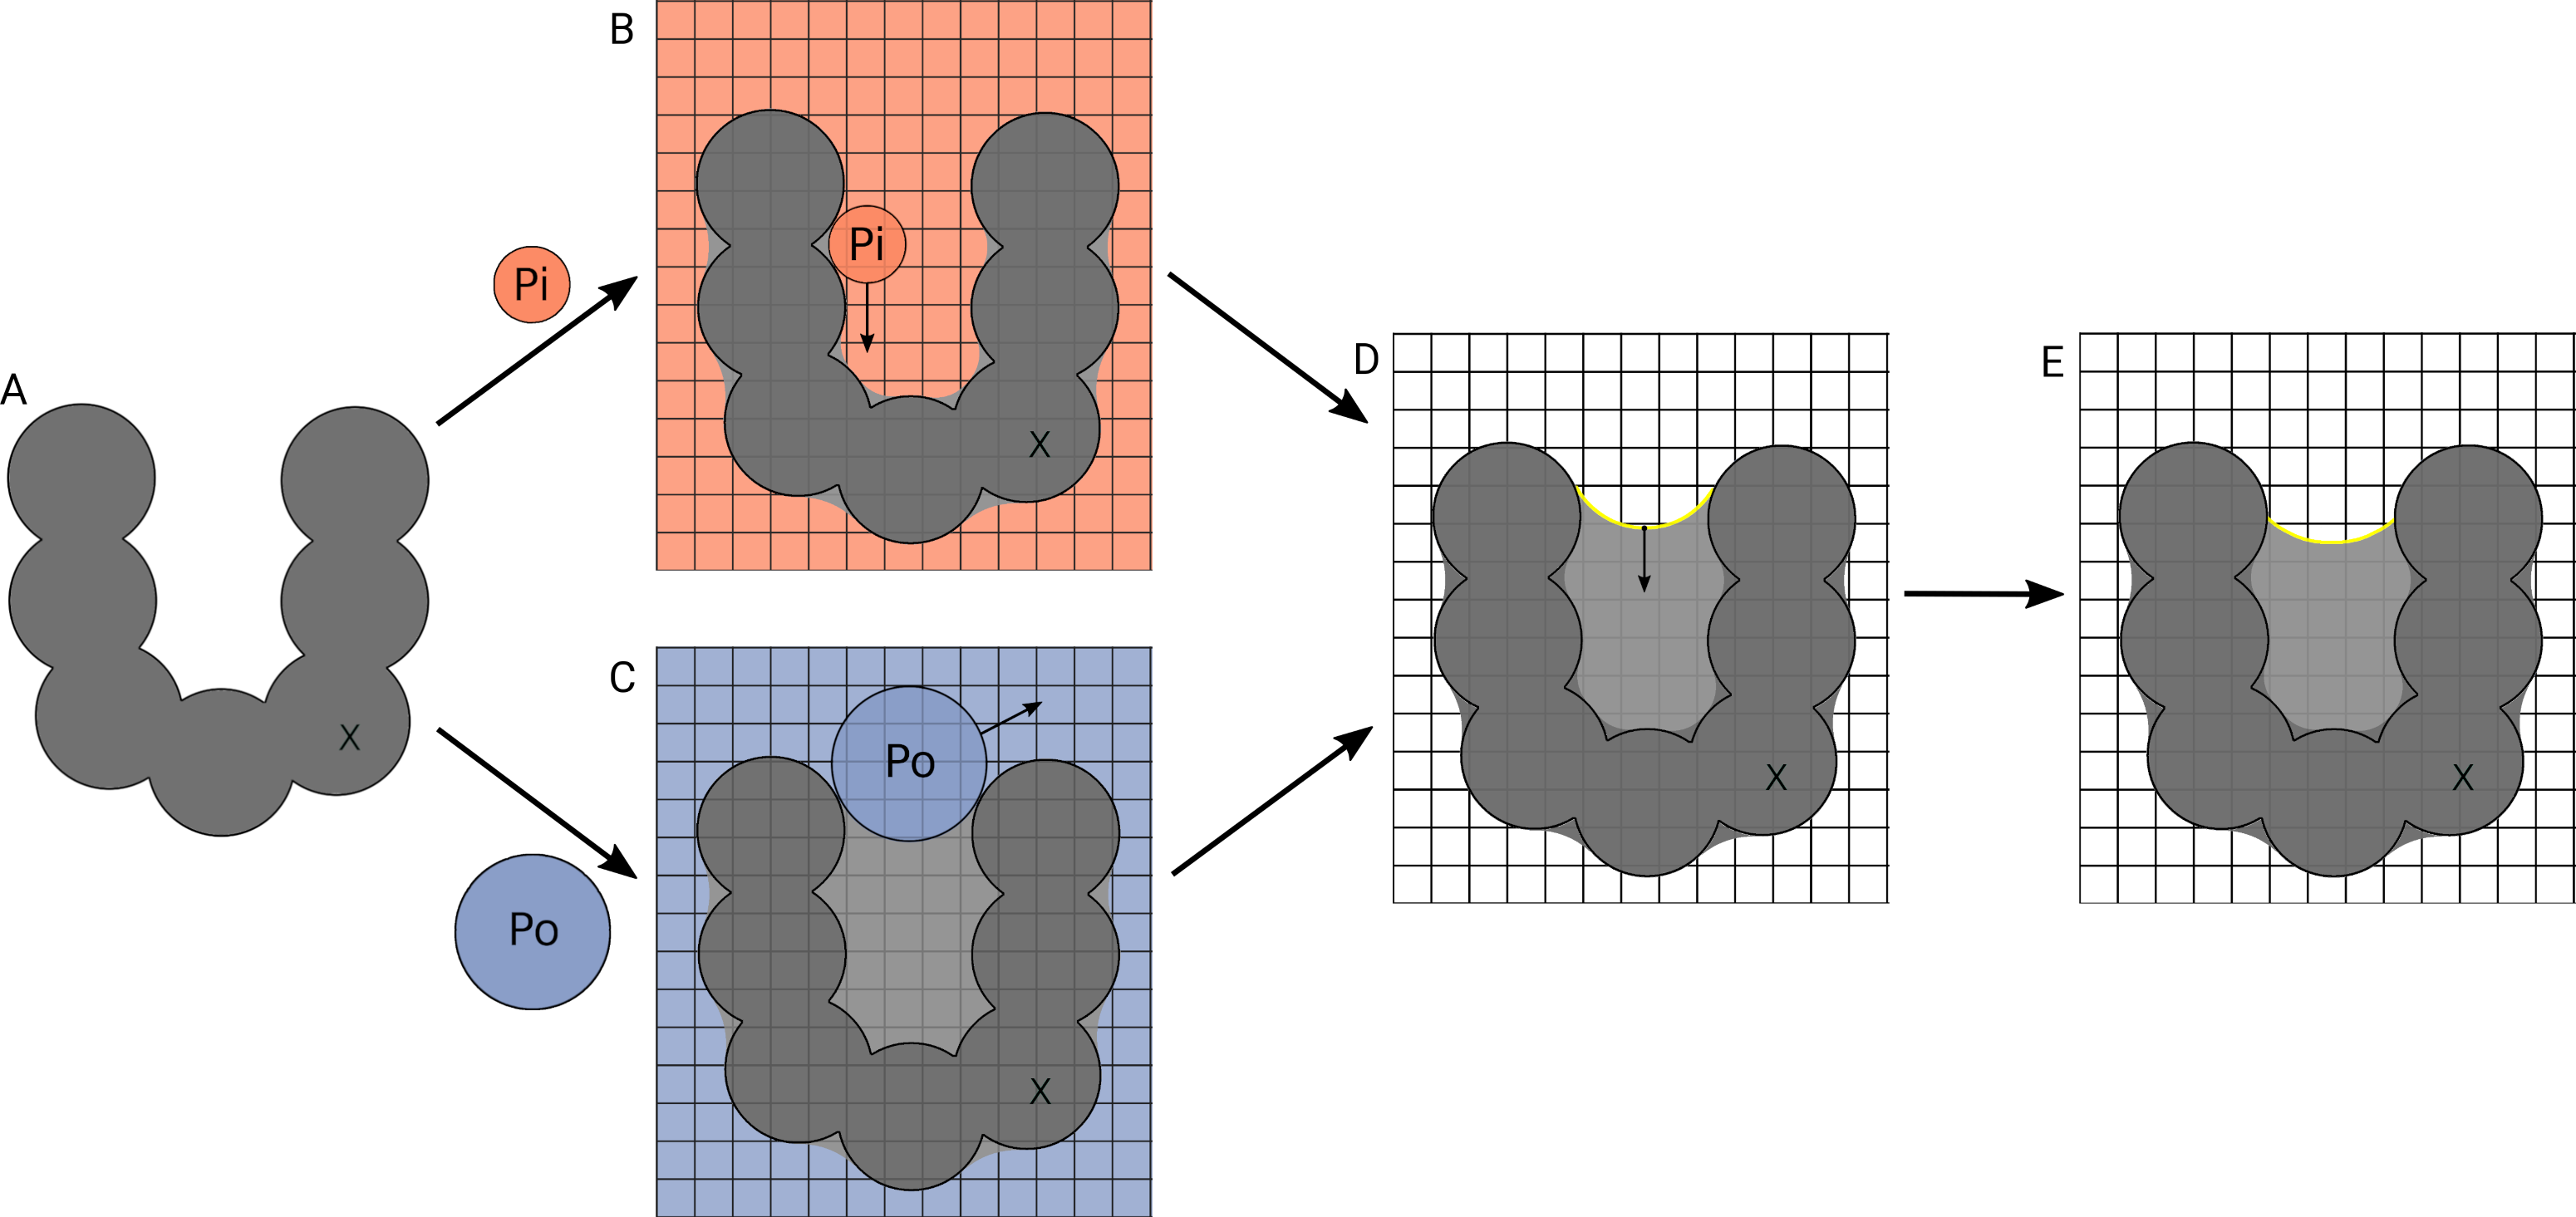
\includegraphics[scale=1]{images/kvfinder-suite-schema.png}}
  \centerline{\scriptsize{\textbf{Fonte:} Retirado de \cite{guerra2023B}.}}
  \caption[Representação esquemática do algoritmo de detecção de cavidades no KVFinder suite]{\textbf{Representação esquemática do algoritmo de detecção de cavidades no KVFinder suite.} \textbf{(A)} Uma estrutura biomolecular X, composta por átomos modelados como esferas rígidas com raios de van der Waals, é inserida em uma grade 3D. \textbf{(B)} A sonda \textit{Probe In} (Pi) percorre a superfície da estrutura, movendo-se pelos pontos da grade (laranja). \textbf{(C)} Em seguida, a sonda \textit{Probe Out} (Po) percorre os pontos acessíveis em azul. \textbf{(D)} Os pontos de cavidade (cinza claro) são definidos como a diferença entre os pontos acessíveis das sondas. Os pontos não alcançados por Pi (cinza escuro) definem a SES (padrão) ou a SAS, dependendo da representação de superfície escolhida pelo usuário. \textbf{(E)} Por fim, é aplicado um procedimento de remoção por distância para eliminar os pontos de cavidade que estão próximos à fronteira da cavidade-solvente (linha amarela).}
  \label{fig:kvfinder-suite-schema}
\end{figure}

É importante destacar que a ferramenta KVFinder \cite{oliveira2014}, originalmente publicada em 2014, está descontinuada. No entanto, novas implementações foram desenvolvidas para aprimorar o desempenho computacional e a usabilidade, resultando nas ferramentas parKVFinder \cite{guerra2020}, pyKVFinder \cite{guerra2021} e KVFinder-web \cite{guerra2023A}. Cada uma dessas ferramentas aborda diferentes demandas da comunidade científica de forma flexível. A caracterização das cavidades nessas ferramentas inclui descritores morfológicos, como volume, área, forma e profundidade, bem como descritores topológicos, como os resíduos de interface que cercam as cavidades, e descritores físico-químicos, como a hidrofobicidade. Para mais informações sobre o KVFinder suite, veja a Seção \ref{sec:kvfinder-suite}.

\subsubsection{Fpocket}

O Fpocket \cite{fpocket} é uma ferramenta baseada em tesselação que realiza a detecção de bolsões com base no conceito de \textalpha-esferas, introduzido por \cite{liang1998}. O algoritmo de detecção de cavidade (Figura \ref{fig:fpocket-schema}) determina o conjunto de \textalpha-esferas a partir da estrutura-alvo, utilizando o pacote \textit{qhull}, e elimina esferas fora de um tamanho de raio mínimo e máximo. As cavidades são agrupamentos de \textalpha-esferas, formadas com base em relações de proximidade e vizinhança, sendo que cavidades não interessantes são removidas da análise posterior. As cavidades restantes são avaliadas usando um conjunto de descritores dpocket \cite{fpocket} e classificadas de acordo com sua suposta capacidade de ligação a uma pequena molécula.

\begin{figure}[ht]
  \centerline{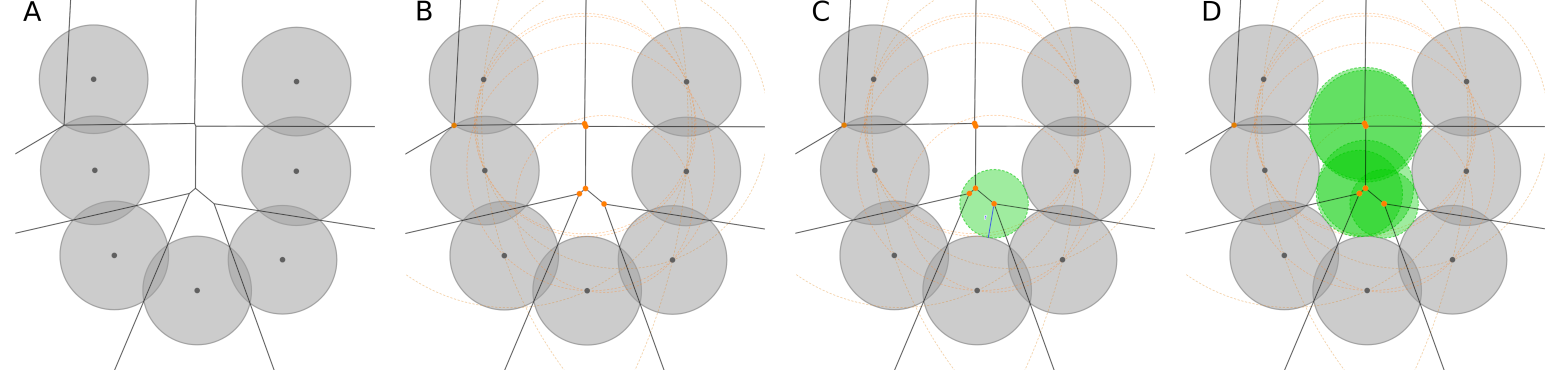
\includegraphics[scale=1]{images/fpocket-schema.png}}
  \centerline{\scriptsize{\textbf{Fonte:} Retirado de \cite{guerra2023B}.}}
  \caption[Representação esquemática do algoritmo de detecção de cavidades no Fpocket]{\textbf{Representação esquemática do algoritmo de detecção de cavidades no Fpocket.} \textbf{(A)} Diagrama de Voronoi dos centros atômicos. \textbf{(B)} Semelhante a uma esfera de Voronoi (círculos laranja pontilhados). \textbf{(C)} Exemplo de uma \textalpha-esfera (região verde); ela é centrada em um vértice de Voronoi (pontos laranja) e cresce até se tornar tangente aos átomos da superfície. \textbf{(D)} Cluster de \textalpha-esferas que preenchem o sítio de ligação.}
  \label{fig:fpocket-schema}
\end{figure}

\subsubsection{GHECOM}

O GHECOM (\textit{Grid-based HECOMi finder}) \cite{ghecom} é uma ferramenta baseada em grade e esfera que detecta bolsos profundos e rasos, utilizando várias sondas esféricas diferentes (Figura \ref{fig:ghecom-schema}). O algoritmo de detecção de cavidade combina operações básicas de erosão e dilatação, da morfologia matemática, com diferentes sondas esféricas para relatar a abertura-fechamento de uma forma molecular-alvo, revelando assim bolsos profundos e rasos (\textit{multi-scale pockets}, em inglês). Dessa forma, um método de agrupamento de ligação simples agrupa regiões de bolsos e posteriormente estima seus volumes. Além disso, o GHECOM relaciona o volume e a profundidade de pontos por resíduo ou átomo em uma métrica chamada \textit{pocketness}, que indica o quanto eles contribuem para a interação com ligantes.

\begin{figure}[H]
  \centerline{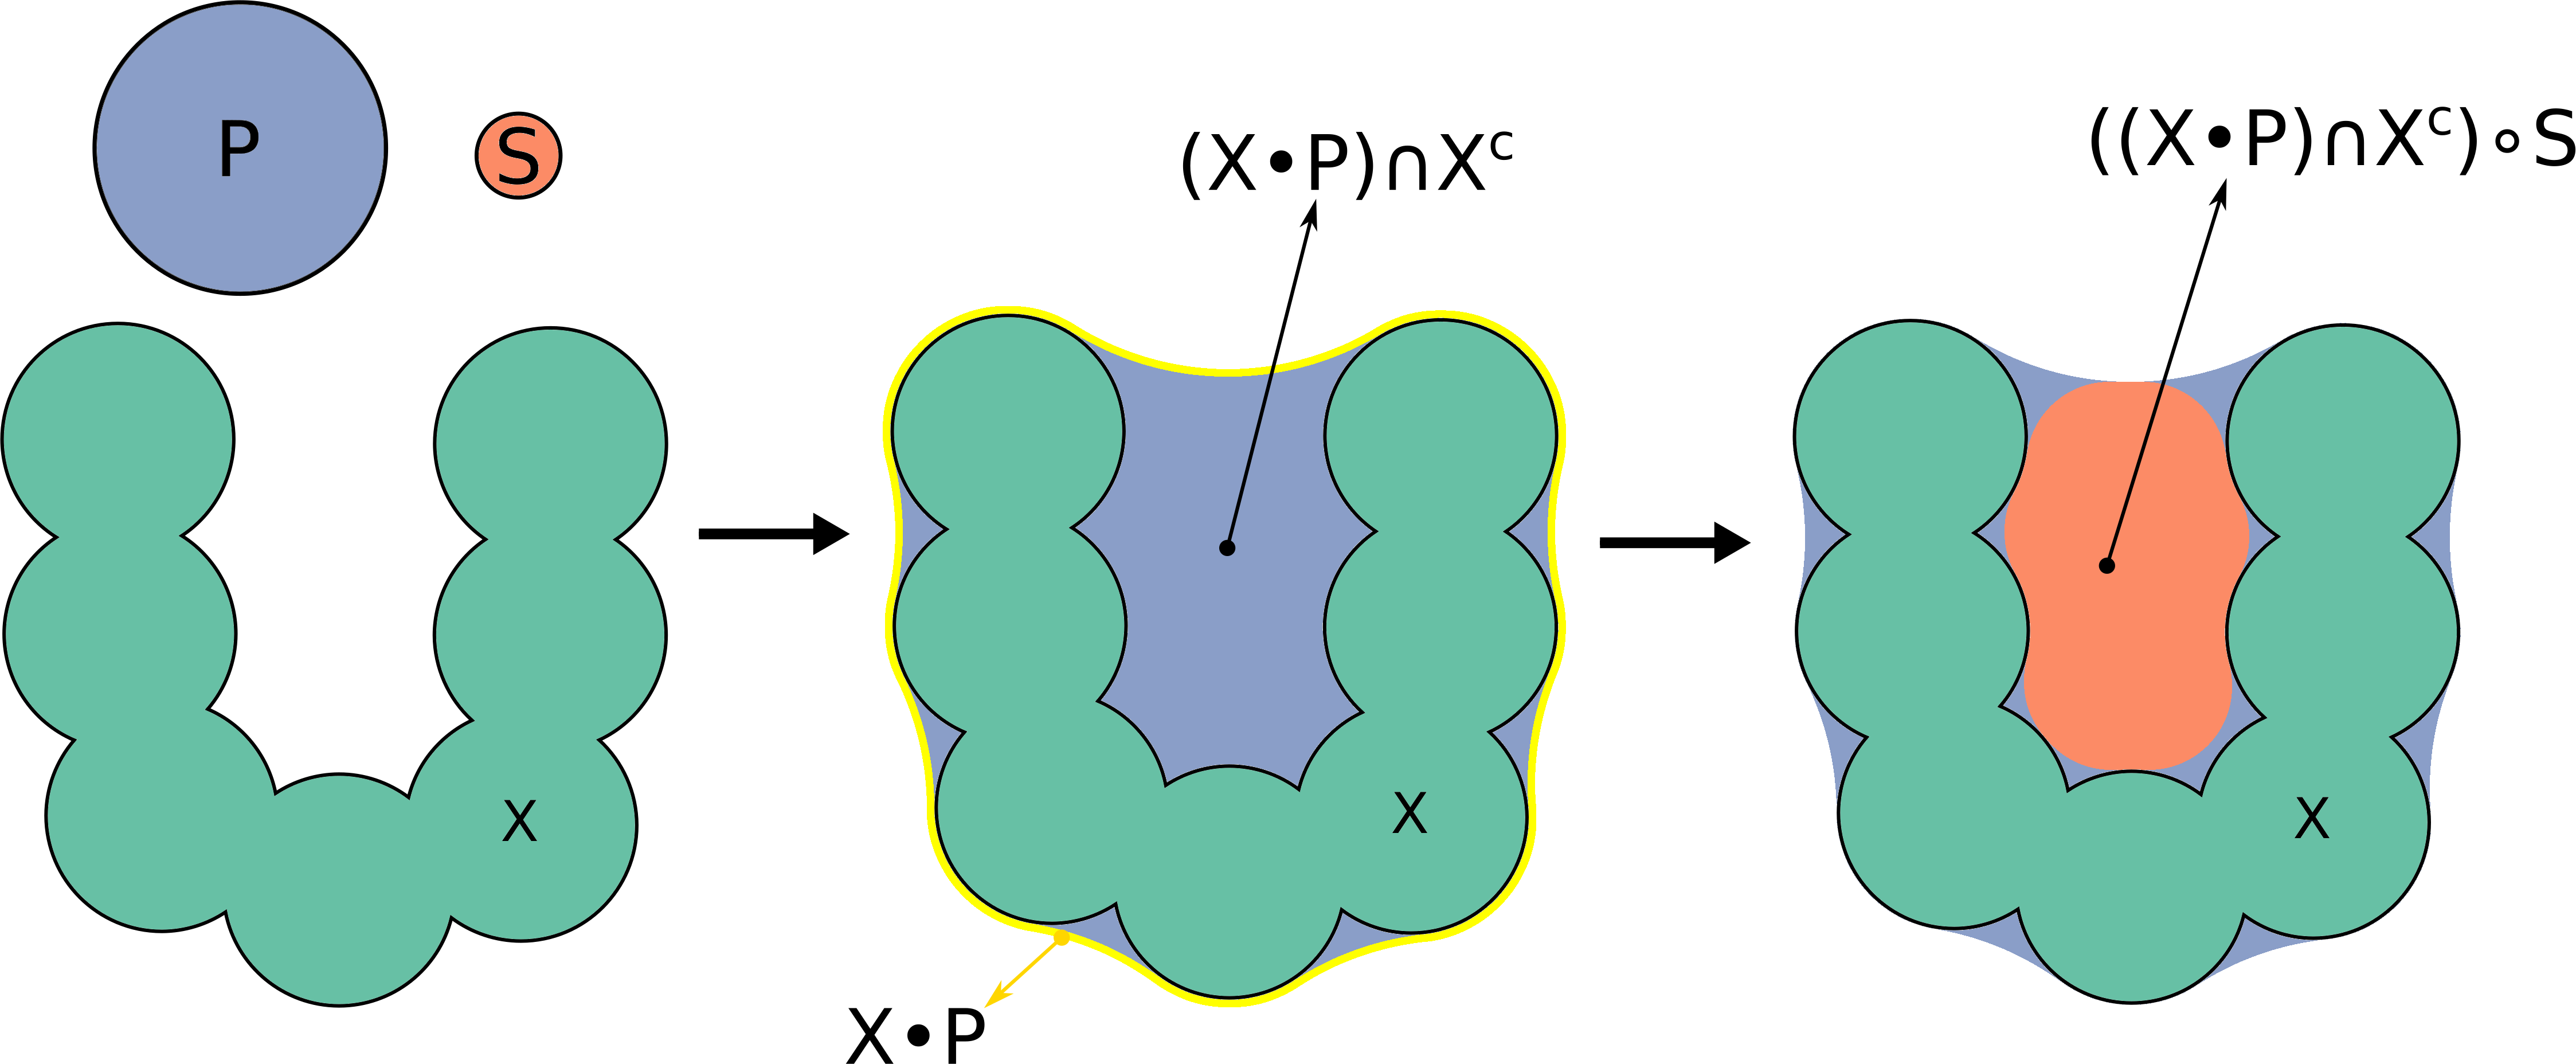
\includegraphics[scale=0.9]{images/ghecom-schema.png}}
  \centerline{\scriptsize{\textbf{Fonte:} Retirado de \cite{guerra2023B}.}}
  \caption[Representação esquemática do algoritmo de detecção de bolsões no GHECOM]{\textbf{Representação esquemática do algoritmo de detecção de bolsões no GHECOM.} Uma estrutura biomolecular (região verde; $X$) é fechada por uma sonda esférica P (esfera azul), definindo a região delimitada pelo contorno amarelo. Em seguida, a interseção de X fechado por P ($X \bullet P$) e o espaço fora da proteína ($X^c$) define a região não acessível à sonda P (região azul; $(X \bullet P) \cap X^c$). Posteriormente, essa região é aberta por uma sonda esférica S (esfera laranja), onde P é maior que S. Por fim, o bolsão (região laranja; $((X \bullet P) \cap X^c) \circ S$) é definido pelo espaço fora da forma molecular não acessível a P, mas acessível a S. Para detecção em múltiplas escalas, são usados diferentes tamanhos da sonda esférica P.}
  \label{fig:ghecom-schema}
\end{figure}

\subsubsection{CAVER}

O CAVER \cite{caver} foi originalmente uma ferramenta baseada em grade e superfície para o cálculo de túneis e canais, que posteriormente foi aprimorada no CAVER 3.0 \cite{caver3}, substituindo a grade alinhada aos eixos por uma abordagem de diagrama de Voronoi. A interface gráfica do usuário, CAVER Analyst 2.0 \cite{caveranalyst2}, incorpora o CAVER 3.0, que auxilia visualmente os usuários nos cálculos de túneis e cavidades. O algoritmo de detecção de cavidades (Figura \ref{fig:caver-schema}) constrói um pseudo-diagrama de Voronoi de uma estrutura biomolecular alvo. A partir dele, o CAVER 3.0 identifica caminhos como grafos compostos por vértices e arestas de Voronoi. Esses caminhos se assemelham a túneis que conectam cavidades ao solvente circundante e são caracterizados por comprimento, raio médio e raio do gargalo. Além disso, CAVER Analyst 2.0 também identifica regiões de espaço vazio, onde uma sonda pequena pode entrar de fora, mas uma sonda grande não pode, aplicando uma abordagem similar às descritas no KVFinder suite (Figura \ref{fig:kvfinder-suite-schema}) e GHECOM (Figura \ref{fig:ghecom-schema}).

\begin{figure}[ht]
  \centerline{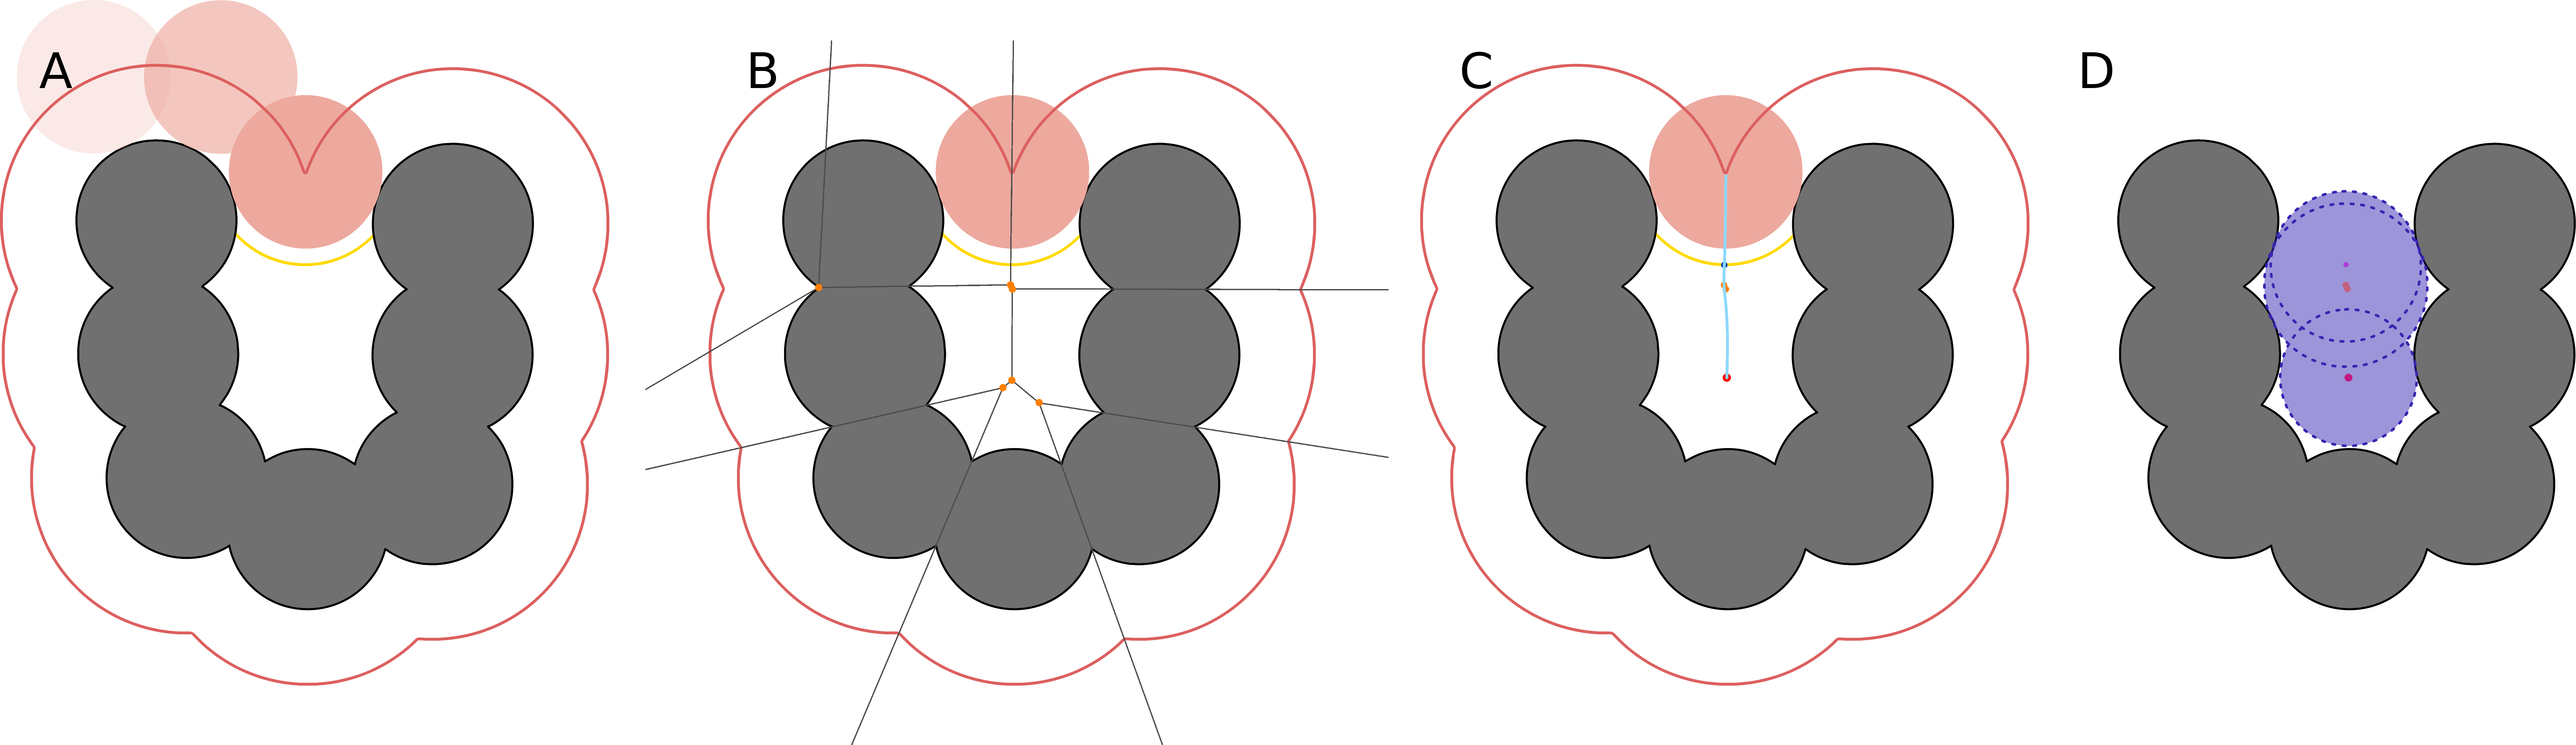
\includegraphics[scale=1]{images/caver-schema.png}}
  \centerline{\scriptsize{\textbf{Fonte:} Retirado de \cite{guerra2023B}.}}
  \caption[Representação esquemática do algoritmo de detecção de canais e túneis no CAVER 3.0 e CAVER Analyst 2.0]{\textbf{Representação esquemática do algoritmo de detecção de canais e túneis no CAVER 3.0 e CAVER Analyst 2.0.} \textbf{(A)} Uma forma molecular é inspecionada por uma sonda esférica, chamada \textit{shell probe}, com um raio especificado pelo parâmetro \textit{shell radius}, para definir uma superfície externa SAS (linha vermelha). A partir dela, uma distância especificada pelo parâmetro \textit{shell depth} é removida para definir uma superfície interna (linha amarela). \textbf{(B)} Um pseudo-diagrama de Voronoi é construído com base na forma molecular. Vértices de Voronoi (pontos laranja) são usados para criar as linhas centrais do túnel/canal. \textbf{(C)} Um ponto de partida (ponto vermelho) é um parâmetro definido pelo usuário, definido como o centro de massa da forma molecular, e um ponto final (ponto azul) é definido no centro da superfície interna. A partir do ponto de partida, a linha central passa por arestas e vértices de Voronoi para formar um túnel/canal até a superfície externa e passa pelo ponto final. \textbf{(D)} Esferas são ajustadas em todos os pontos da linha central, do ponto de partida ao ponto final, o que define o raio do gargalo (abertura) ao longo do túnel e/ou canal.}
  \label{fig:caver-schema}
\end{figure}

% Melhorias para a Defesa:
% - Caracterização de cavidades: describe importance of cavity characterization to identify functionally relevant cavities and how to do it

%%% Chapter 2

\chapter{Objetivos}

\section{Objetivo geral}

Este trabalho tem como objetivo o desenvolvimento de uma plataforma computacional, denominada \textbf{KVFinder suite}, para estudo de sistemas biomoleculares em biologia estrutural.

\section{Objetivos específicos}

Os objetivos específicos incluem: (1) Aprimoramento e desenvolvimento de descritores de propriedades do KVFinder suite; (2) Implementação de diferentes codificações para biomoléculas e sítios de ligação; (3) Desenvolvimento de ferramenta para ciência de dados e protocolos automatizados; (4) Desenvolvimento de um serviço \textit{web} para análise de sítios de ligação; (5) Desenvolvimento de um programa para representação em forma de grafos de interface de interação de biomoléculas; e (6) Desenvolvimento de ferramenta para análises de dinâmica molecular.

%%% Chapter 3

\chapter{Codificação de biomoléculas e seus sítios de ligação}

A codificação de biomoléculas e sítios de ligação desempenha papel fundamental na biologia estrutural, permitindo a representação e análise computacional de informações biológicas complexas. Esse processo converte informações biológicas em formatos compreensíveis e adequados para processamento por algoritmos e programas em sistemas computacionais. A codificação envolve a atribuição de valores ou categorias aos componentes biológicos, \eg, átomos, aminoácidos e bases nitrogenadas, para descrever ocupância, localização, forças, características físico-químicas e/ou propriedades estruturais. 

Na biologia estrutural, a codificação de dados é importante para realizar análises avançadas, \eg, modelagem molecular, simulações de dinâmica molecular (DM) e predição de interações. Existem várias aplicações que exemplificam a codificação de dados biológicos para análises computacionais. Por exemplo, na modelagem molecular, uma proteína pode ser codificada usando códigos de uma letra para representar os diferentes aminoácidos, como ocorre na representação de sequência de proteínas, para predizer o dobramento de proteínas, como aplicado no ESMFold \cite{lin2022}. Na simulação de DM, as coordenadas 3D de átomos ou conjunto de átomos, juntamente com vetores que representam forças ou outros atributos, são utilizados para representar a estrutura de uma biomolécula, como no GROMACS \cite{gromacs} ou AMBER \cite{amber} em simulações em escala atomística (\textit{fine-grained molecular dynamics simulation}, em inglês) e no CafeMol em simulações em escala grosseiras (\textit{coarse-grained molecular dynamics simulation}, em inglês) \cite{kenzaki2011}. Além disso, os sítios de ligação, após identificados por algoritmos computacionais, são codificados de diferentes maneiras para análises posteriores. Os sítios de ligação podem ser codificados para representar as características físico-químicas e estruturais de uma região de uma biomolécula, como as grades 3D utilizadas no KVFinder suite \cite{oliveira2014,guerra2020,guerra2021,guerra2023B}, ou as coordenadas 3D dos átomos, como no fpocket \cite{fpocket}.

Ao trabalhar com modelos computacionais para o estudo de biomoléculas, a codificação é essencial para a abstração e representação dos dados biológicos de forma computacional. Essa abstração é crucial para o desenvolvimento de ferramentas computacionais voltadas ao estudo de sistemas biomoleculares. Aqui, apresentamos as codificações implementadas para biomoléculas e sítios de ligação, \ie, representação em grade 3D, representação topológica e representação em grafos.

\section{Representação em grade tridimensional}

As biomoléculas e seus sítios de ligação podem ser representadas em uma grade 3D subdividida em voxels (\textit{volumetric pixel}, em inglês). A grade 3D é uma estrutura de dados que armazena valores em uma matriz tridimensional, onde cada elemento da matriz é denominado voxel. O voxel representa um ponto discreto de dados em uma grade regular no espaço tridimensional, sendo que cada ponto pode conter mais de uma informação a fim de representar diferentes propriedades em uma certa porção de espaço de maneira simples e efetiva (Figura \ref{fig:voxel}). Em computação, a grade 3D é uma estrutura de dados comumente utilizada em aplicações de processamento de imagens e visão computacional, como em reconstrução de imagens, segmentação de imagens e detecção de objetos. 

\begin{figure}[ht]
  \centerline{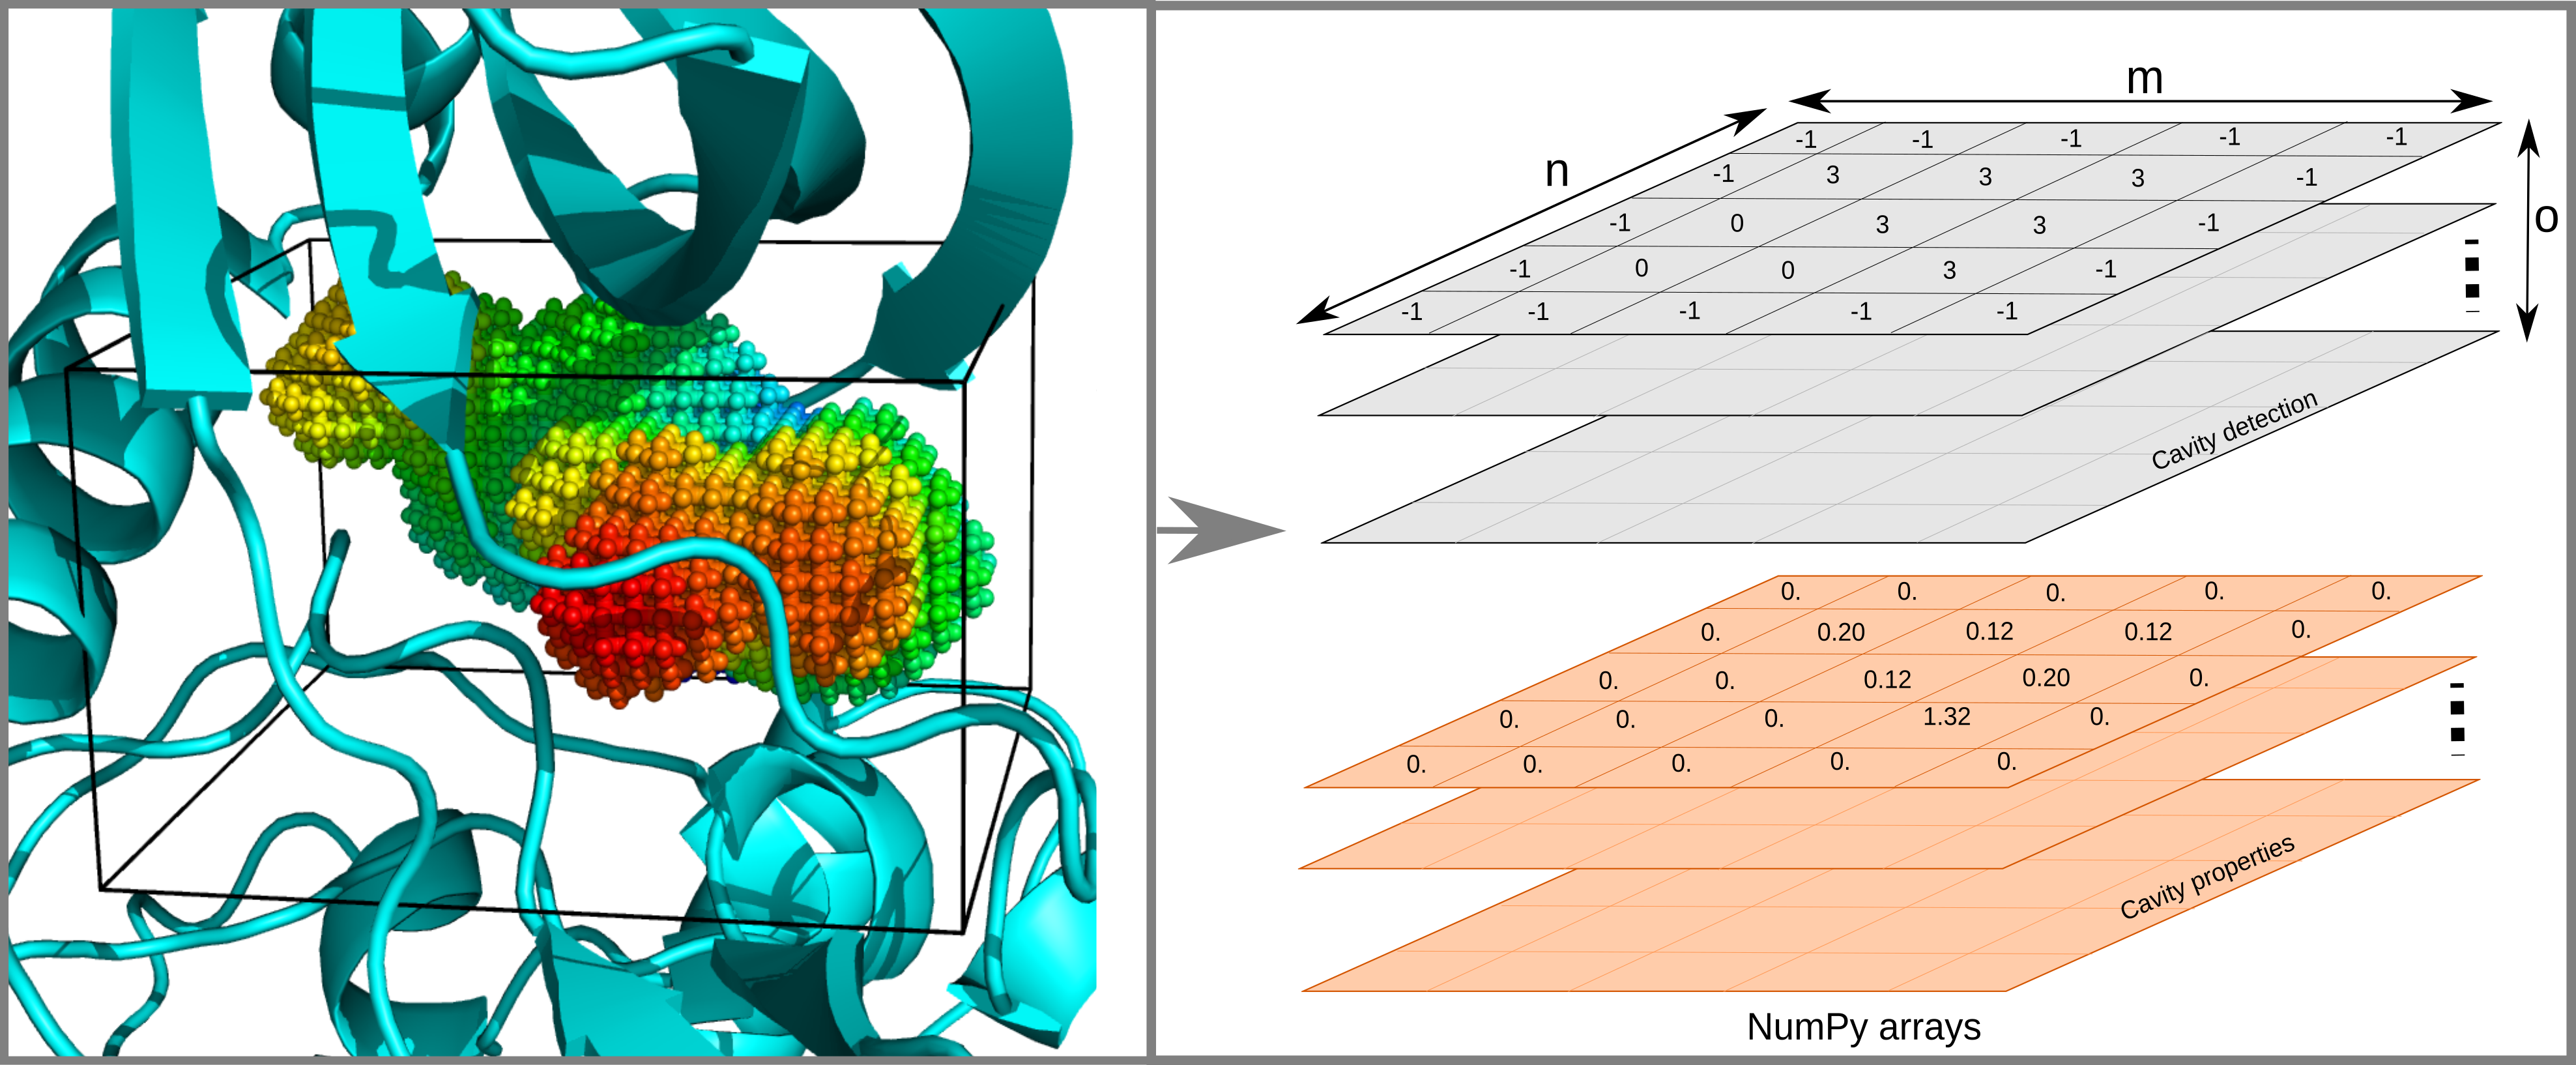
\includegraphics[scale=1]{images/voxels.png}}
  \centerline{\scriptsize{\textbf{Fonte:} Retirado de \cite{guerra2021}.}}
  \caption[Representação esquemática de biomoléculas e seus sítios de ligação representadas em grade tridimensional]{\textbf{Representação esquemática de biomoléculas e seus sítios de ligação representadas em grade tridimensional.} Com base em uma grade tridimensional com dimensões (m, n, o), cada elemento corresponde a uma região de cavidade (>1), espaço vazio (1), biomolécula (0) ou solvente (-1). Além disso, propriedades também são armazenadas na mesma estrutura de dados, correspondendo ao valor da propriedade na região.}
  \label{fig:voxel}
\end{figure}

Dentre as diversas representações de superfície molecular, a grade tridimensional composta por voxels é a mais simples e apropriada para a representação de múltiplas propriedades em várias condições, pois cada voxel da grade tridimensional pode acumular diferentes informações. Além disso, a grade 3D é uma estrutura de dados eficiente para armazenar e acessar valores e/ou atributos em uma posição 3D, permitindo a realização de operações matemáticas e lógicas em uma região 3D. 

% Essa representação é útil para identificar regiões de interesse em biomoléculas, como sítios de ligação, e para realizar análises de propriedades físico-químicas e estruturais, como a distribuição de cargas e a distribuição de propriedades hidrofóbicas. 

\subsection{Representação de superfícies moleculares}

A representação de superfícies moleculares é uma etapa fundamental na modelagem e análise de biomoléculas. Nessa abordagem, as biomoléculas são descritas por meio de um modelo de esfera rígida, que considera as posições e raios atômicos para representar a superfície molecular. Existem três formulações matemáticas comumente utilizadas para representar as superfícies moleculares (Figura \ref{fig:surface-representation}):

\begin{enumerate}[label=\textbf{(\Alph*)}]
  \item \textbf{superfície de vdW:} representa cada átomo por uma esfera cujo raio é proporcional ao seu raio de van der Waals. A superfície de vdW é representada como a união desses átomos esféricos; 
  \item \textbf{SAS:} representa as regiões de uma molécula que podem ser acessadas por uma molécula de solvente (\eg, uma molécula de água), que é aproximada por uma sonda esférica;
  \item \textbf{SES:} é semelhante ao SAS, mas considera-se a casca externa da sonda, em vez do centro da sonda.
\end{enumerate}

\begin{figure}[ht]
  \centerline{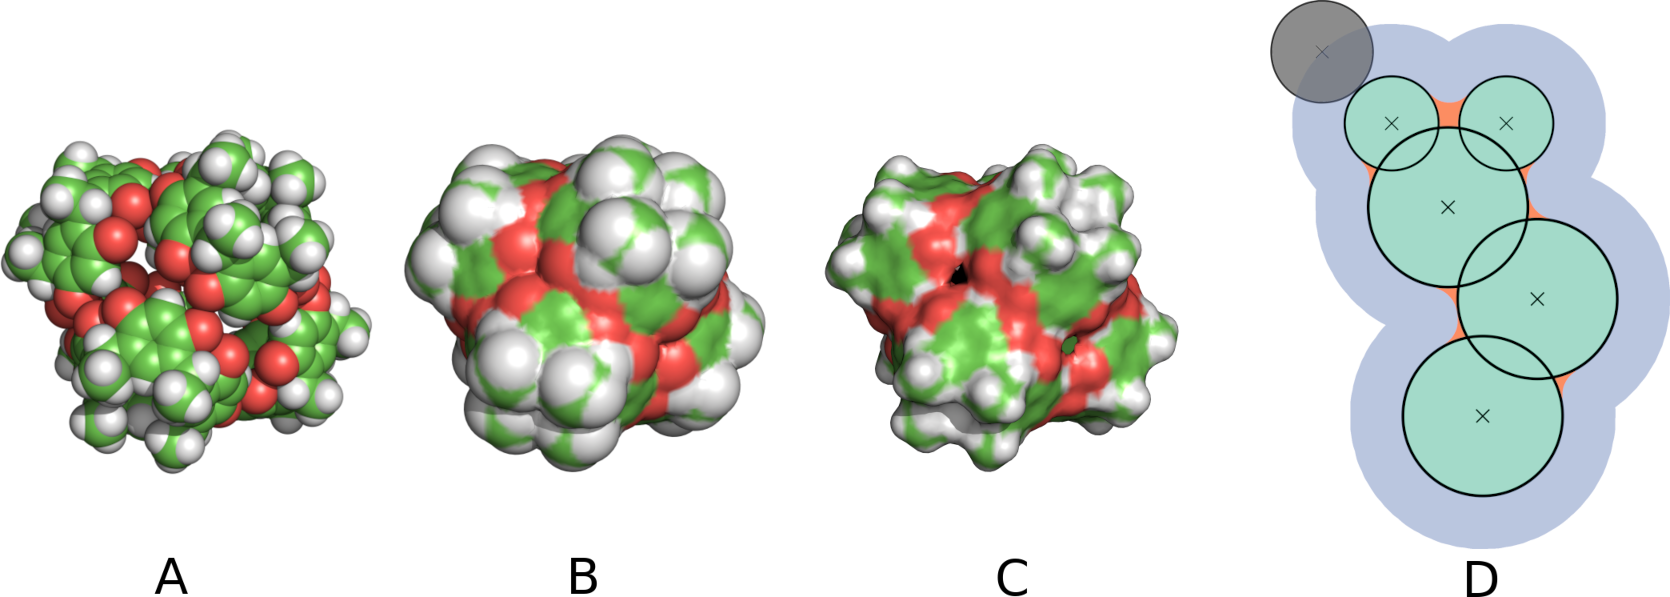
\includegraphics[scale=1]{images/surface-representation.png}}
  \centerline{\scriptsize{\textbf{Fonte:} Retirado de \cite{guerra2023B}.}}
  \caption[Representações de superfície molecular]{\textbf{Representações de superfície molecular.} \textbf{(A)} Superfície de vdW. \textbf{(B)} SAS. \textbf{(C)} SES. Imagens geradas com PyMOL para a gaiola supramolecular (resorcin[4]areno-hexamérica). \textbf{(D)} Representação esquemática 2D das superfícies moleculares. A superfície de vdW (verde) é composta por átomos representados como esferas verdes. Uma sonda esférica (cinza), representando uma molécula de solvente, rola sobre os átomos da molécula para definir SES e SAS. O SES é definido pela superfície de vdW (verde) e pelo espaço não alcançado pela sonda esférica (laranja). O SAS é definido pelo envelope alcançado pelo centro da sonda esférica (azul).}
  \label{fig:surface-representation}
\end{figure}

\section{Representação pela topologia}

% Melhorias para a Defesa:
% - Descrever implementação: Lista de listas (em Python) com informações sobre átomos, aminoácidos e/ou bases nitrogenadas.

Em vez de representar os dados estruturais por meio de voxels em uma grade 3D, as biomoléculas e seus sítios de ligação também podem ser representados por sua topologia (Figura \ref{fig:topology-representation}), seguindo abordagens semelhantes às simulações de DM, como GROMACS \cite{gromacs}, AMBER \cite{amber} e CafeMol \cite{kenzaki2011}. Nessa representação, átomos, resíduos e/ou bases nucleotídicas são modelados como esferas rígidas (\textit{hard sphere models}, em inglês) com coordenadas 3D (x, y, z), juntamente com vetores (\eg, forças, velocidades e acelerações) e propriedades (\eg, massa, carga e raio de vdW).

\begin{figure}[ht]
  \centerline{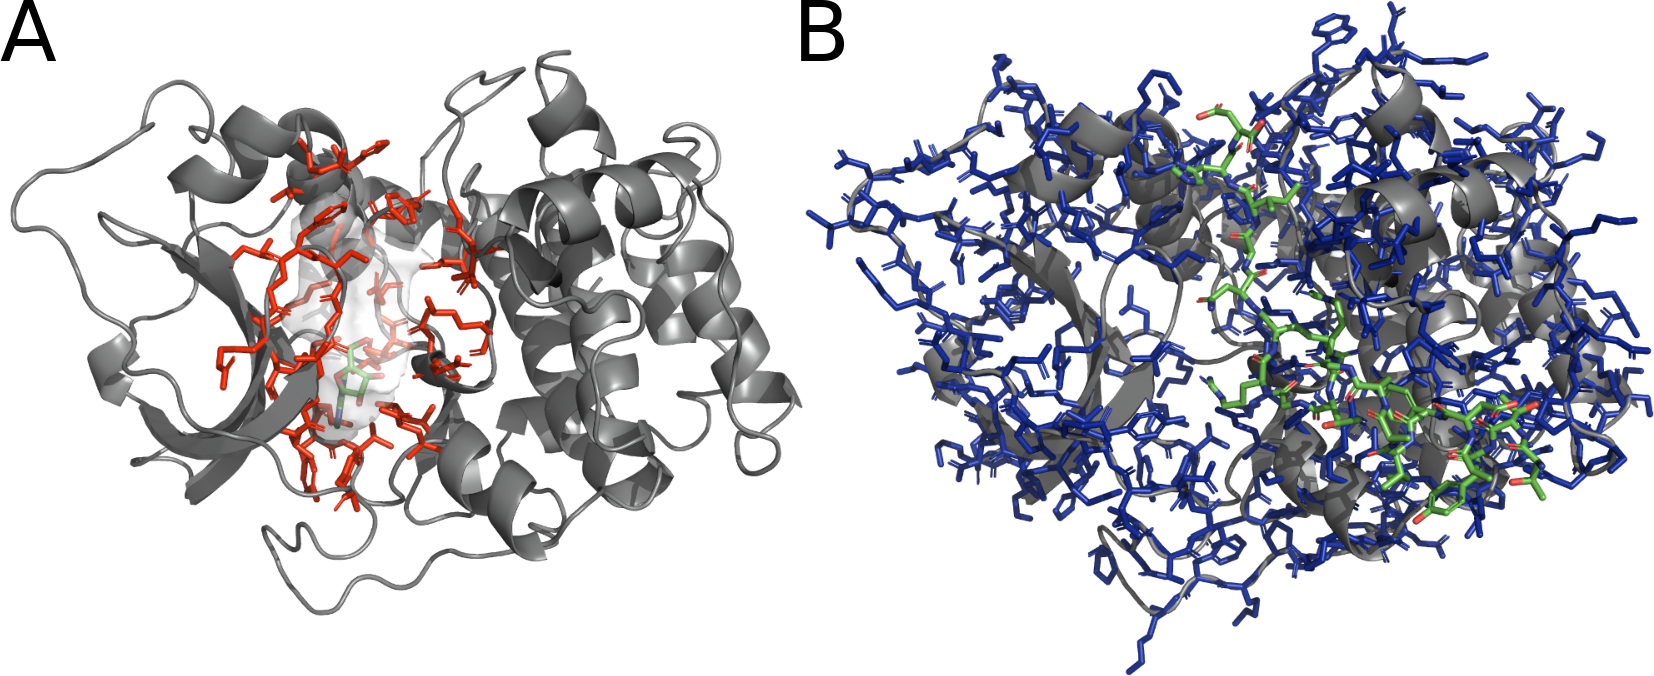
\includegraphics[scale=2]{images/topology-representation.png}}
  \caption[Representações topológicas de interfaces de interação em estruturas biomoleculares]{\textbf{Representações topológicas de interfaces de interação em estruturas biomoleculares.} \textbf{(A)} Átomos e aminoácidos (\textit{sticks} em verde) que formam o sítio de ligação da adenosina (superfície transparente). \textbf{(B)} Átomos e aminoácidos (\textit{sticks} em azul) expostos ao solvente, que excluem sítios de ligação para pequenas moléculas, com um inibidor ligado (\textit{sticks} em verde). Imagens geradas com PyMOL para uma subunidade da proteína quinase CAMP-dependente (PDB ID: 1FMO).}
  \label{fig:topology-representation}
\end{figure}

Porém, ao estudarmos regiões de interação, é necessário filtrar as áreas de interesse, como sítios de ligação (Figura \ref{fig:topology-representation}A) ou superfície exposta ao solvente (Figura \ref{fig:topology-representation}B), para realizar análises estruturais e funcionais específicas. Essa representação topológica permite análises direcionadas, focando nas interações e características estruturais relevantes para a função biológica. Além disso, as informações topológicas podem ser utilizadas em estudos de acoplamento molecular (\textit{molecular docking}, em inglês), desenho racional de fármacos e predição de interações moleculares. Essas aplicações contribuem para o desenvolvimento de novos compostos terapêuticos e auxiliam na compreensão dos mecanismos moleculares envolvidos em processos biológicos.

Dessa forma, a representação topológica das biomoléculas e seus sítios de ligação proporciona uma visão detalhada e especializada das características estruturais relevantes, permitindo uma análise mais precisa e aprofundada das interações moleculares e seu impacto na função biológica.

\section{Representação em grafos \label{sec:graph-representation}}

% Melhorias para a Defesa:
% - Figura de grafos genéricos para a Defesa
% - Expandir sobre os tipos de grafos: direcionados, não-direcionados, ponderados, etc.
% - Expandir sobre as propriedades em vértices e arestas
% - Expandir sobre as aplicações de grafos em biologia

A representação de interações ou relações entre elementos por meio de grafos é uma abordagem que tem sido utilizada em diversas áreas, como biologia, química, física, ciência da computação e matemática \cite{foulds1995,majeed2020}. Grafos são estruturas de dados poderosas e flexíveis que podem ser usadas para representar e analisar relações e interações entre elementos. No contexto de biomoléculas, essa representação já foi utilizada para investigar a estrutura, dobramento, estabilidade, função e dinâmica de proteínas \cite{vishveshwara2002}.

Grafos são estruturas matemáticas compostas por um conjunto de vértices (também chamados de nós) e um conjunto de arestas que conectam esses vértices. No caso de moléculas, que são conjuntos de átomos (vértices) conectados por interações intramoleculares e intermoleculares (arestas), também têm sido amplamente investigadas pela teoria dos grafos \cite{vishveshwara2002,mason2007}.

A representação de grafos implementada utiliza as coordenadas 3D (x, y, z) de uma estrutura ou complexo biomolecular e gera um grafo de resíduos, onde os vértices representam os resíduos e as arestas representam interações ou algum tipo de relação entre eles. A construção das arestas é baseada em cortes de distância customizáveis entre os átomos, como carbono \textalpha, carbono \textbeta\space ou qualquer outro átomo, que podem ser definidos pelo usuário (Figura \ref{fig:serd-graph}). Os parâmetros padrões definidos na implementação são uma distância de corte de 10 Å entre átomos carbono \textalpha, de 8 Å entre átomos carbono \textbeta\space (ou carbono \textalpha\space para glicina), e de 5 Å entre quaisquer dois átomos são estabelecido para definir relação ou interação entre resíduos, respectivamente \cite{vishveshwara2002,mason2007}. A Figura \ref{fig:serd-graph}A mostra um exemplo de grafo de resíduos gerado a partir de um sítio de ligação da adenosina (Figura \ref{fig:topology-representation}A) e a Figura \ref{fig:serd-graph}B mostra um exemplo de grafo de resíduos gerado a partir de uma superfície exposta ao solvente (Figura \ref{fig:topology-representation}B).

% Ref CB e all-atoms: https://www.ebi.ac.uk/msd-srv/capri/round28/round28.html

\begin{figure}[ht]
  \centerline{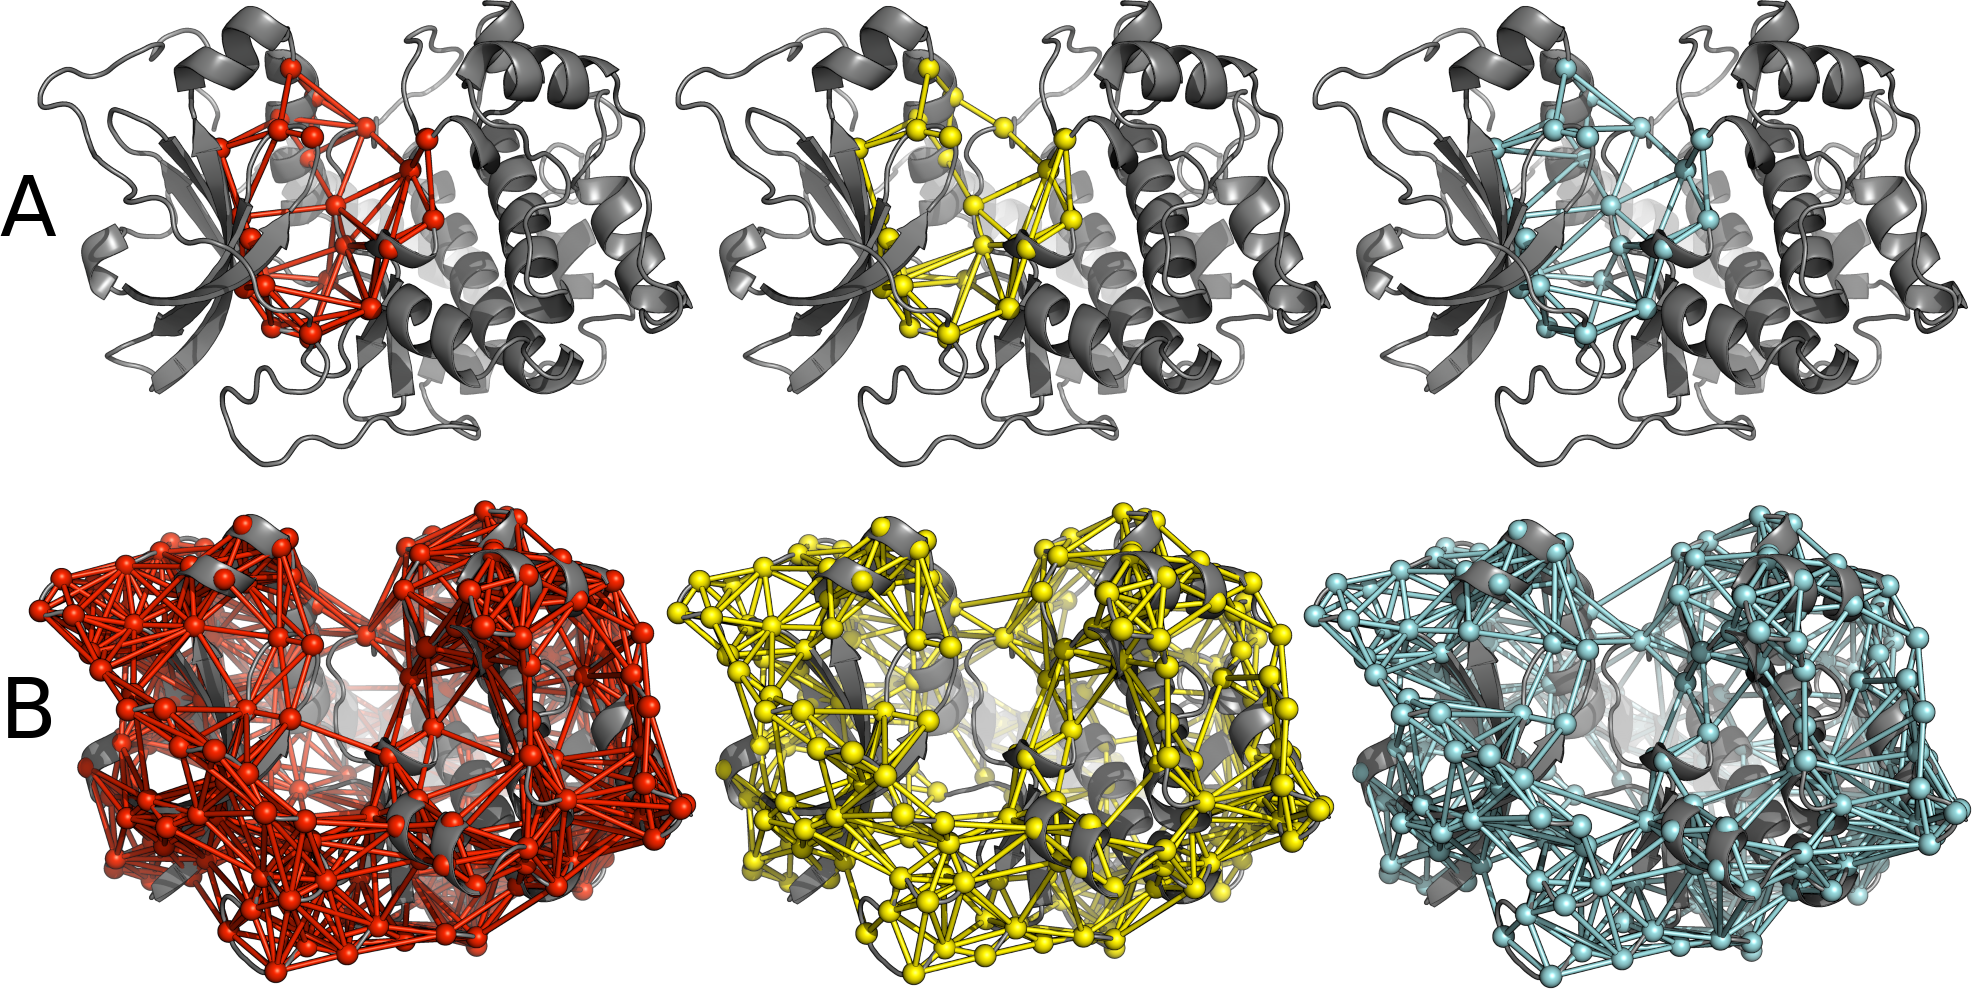
\includegraphics[scale=1.9]{images/graph-representation.png}}
  \caption[Representações em forma de grafos em estruturas biomoleculares]{\textbf{Representações em forma de grafos em estruturas biomoleculares.} \textbf{(A)} Sítio de ligação da adenosina como grafos com arestas baseados no corte de distância de carbono \textalpha\space (esferas e bastões em vermelho), carbono \textbeta\space (esferas e bastões em amarelo) e qualquer átomos dos resíduos (esferas e bastões em ciano). \textbf{(B)} Superfície exposta ao solvente, que excluem sítios de ligação para pequenas moléculas, como grafos com arestas baseados no corte de distância de carbono \textalpha\space (esferas e bastões em vermelho), carbono \textbeta\space (esferas e bastões em amarelo) e qualquer átomos dos resíduos (esferas e bastões em ciano). Imagens geradas com PyMOL para uma subunidade da proteína quinase CAMP-dependente (PDB ID: 1FMO).}
  \label{fig:serd-graph}
\end{figure}

Essa representação em grafos permite uma análise mais simplificada e eficiente das interações e relações entre os resíduos, proporcionando uma visualização clara das características estruturais e funcionais da biomolécula. Além disso, diversas propriedades e medidas podem ser calculadas a partir dos grafos, como caminhos, distâncias, centralidade e outras métricas que auxiliam na compreensão da estrutura e função da biomolécula \cite{majeed2020,vishveshwara2002,mason2007}. Em resumo, a representação em grafos é uma abordagem poderosa e versátil para analisar a estrutura e as interações em biomoléculas, permitindo uma compreensão mais aprofundada de sua função biológica e fornecendo \textit{insights} importantes para o desenvolvimento de terapias e intervenções terapêuticas.

%%% Chapter 4

\chapter{Plataforma KVFinder suite \label{sec:kvfinder-suite}}

% https://cnpemcamp-my.sharepoint.com/:w:/r/personal/joao_guerra_lnbio_cnpem_br/_layouts/15/Doc.aspx?sourcedoc=%7BD0C80180-AF7E-412F-B94E-6C38D8D4C946%7D&file=Relat%C3%B3rio%20Plataforma%20Biologia%20Computacional%202022.2.docx&action=default&mobileredirect=true

As interações entre biomoléculas desempenham um papel crucial em processos biológicos, envolvendo desde pequenas moléculas, como íons e fármacos, até macromoléculas, como proteínas e ácidos nucleicos. Essas interações receptor-ligante (\eg, IPPs, IPLs, IPRs e IPDs) ocorrem em sítios de ligação específicos, que podem ser fendas expostas ao solvente ou cavidades enterradas nos receptores. A complementariedade espacial, estrutural e físico-química entre os ligantes e receptores governa o reconhecimento molecular, restringindo a interação eficiente a um número limitado de ligantes. A identificação e avaliação dessas regiões são fundamentais para o entendimento da estrutura terciária da biomolécula e para o desenvolvimento de novos fármacos. Para atender a essa demanda, desenvolvemos a plataforma computacional \textbf{KVFinder suite}, que combina ferramentas precisas com processamento de alto desempenho, permitindo a análise de dados experimentais biomoleculares e a compreensão da estrutura e função das biomoléculas em sistemas biológicos.

A KVFinder suite é composta por cinco ferramentas computacionais que oferecem funcionalidades abrangentes para análise estrutural e estudo de interações biomoleculares. As ferramentas incluídas na plataforma são: parKVFinder \cite{guerra2020}, pyKVFinder \cite{guerra2021}, KVFinder-web \cite{guerra2023A}, SERD e KVFinderMD. A seguir, descreveremos cada uma dessas ferramentas e suas principais características.

\section{parKVFinder}

O \textbf{Parallel KVFinder (parKVFinder)} \cite{guerra2020} é uma ferramenta de código aberto, licenciada sob GPL v3.0, desenvolvida para detecção e caracterização de qualquer tipo de cavidade biomolecular. A ferramenta foi desenvolvida originalmente na dissertação de mestrado intitulada "Prospecção e caracterização de cavidades supramoleculares" \cite{guerra2019}, como uma versão atualizada e otimizada do KVFinder \cite{oliveira2014}. Posteriormente, o parKVFinder foi publicado na SoftwareX \cite{guerra2020}, aprimorando a estimativa de área superficial, sendo lançado como \href{https://github.com/LBC-LNBio/parKVFinder/tree/v1.0}{parKVFinder v1.0}. Em seguida, houve uma nova atualização para o KVFinder-web \cite{guerra2023A}, adicionando os descritores de profundidade, hidrofobicidade e frequência de resíduos, resultando no lançamento do \href{https://github.com/LBC-LNBio/parKVFinder/tree/v1.2.0}{parKVFinder v1.2.0}.

O parKVFinder é acompanhado por um plugin gráfico, denominado PyMOL2 parKVFinder Tools, que é integrado ao visualizador molecular PyMOL \cite{pymol}. Esse plugin oferece uma interface gráfica intuitiva e fácil de usar, permitindo que os usuários explorem parâmetros personalizáveis para a detecção e caracterização de cavidades. Além disso, o plugin permite visualizar as cavidades detectadas e suas características no ambiente do PyMOL. Além da interface gráfica, o parKVFinder também possui uma interface de linha de comando (CLI; \textit{command-line interface}) para usuários avançados, o que permite a automação de tarefas e a integração com outros programas. O código-fonte do parKVFinder e o plugin estão disponíveis no seguinte repositório: \url{https://github.com/LBC-LNBio/parKVFinder}.

As rotinas de detecção e caracterização de cavidades foram paralelizadas utilizando a biblioteca OpenMP, aproveitando o processamento paralelo em sistemas \textit{multicore}. O desempenho computacional do parKVFinder foi avalidado em um conjunto de 1000 domínios proteicos, denominado kv1000 (\url{https://github.com/jvsguerra/kv1000}), apresentando um tempo de execução consideravelmente menor que o KVFinder, $\aproximadamente9{,}5$ vezes mais rápido \cite{guerra2019,guerra2020}.

% Melhorias defesa:
% - Detalhar comparação com outros métodos
% - Detalhar atualização para Python3 do plugin

\subsection{Casos de estudo}

O parKVFinder foi aplicado em dois casos de estudo publicados em periódicos científicos para investigar proteínas de interesse terapêutico. Essas análises exploraram a dinâmica dos \textit{flaps} da protease do Vírus da imunodeficiência humana 1 (HIV-1; \textit{Human Immunodeficiency Virus type 1}, em inglês) \cite{guerra2020} e o caráter hidropático de sítios de ligação em alphavírus \cite{ribeiro2021}. No apêndice \ref{ap:casos-de-estudo-parkvfinder}, descreveremos cada um desses casos de estudo em detalhes.

% A seguir, descreveremos cada um desses casos de estudo em detalhes.

\subsection{Discussão}

Apesar de termos obtido sucesso na aplicação do parKVFinder em simulações de DM \cite{guerra2020} e em um estudo comparativo \cite{ribeiro2021}, encontramos limitações ao utilizá-lo em aplicações automatizadas e comparações sistemáticas de sítios de ligação. Por essa razão, é necessário uma ferramenta mais apropriada para aplicações em ciência de dados, que ofereça um acesso simplificado a funções e estruturas de dados durante a análise. No entanto, é importante destacar que o parKVFinder ainda desempenha um papel importante na plataforma do KVFinder suite, principalmente na otimização dos parâmetros de detecção e caracterização, por meio do plugin gráfico do PyMOL (PyMOL2 parKVFinder Tools), devido aos seus recursos visuais. Estes parâmetros otimizados podem ser posteriormente adotados em estudos automatizados e comparações sistemáticas de sítios de ligação. Por fim, o parKVFinder também continua sendo útil para análises estrutural e funcional focadas em uma única estrutura biomolecular.

% Extra information:
% - Given the relevance of E1–E2 ectodomains in host cell infection and induction of humoral immune responses, we compared the MAYV structure to CHIKV. These alphaviruses are closely related, cause similar diseases, and induce serological cross-reactivity that complicates diagnosis. 

\section{pyKVFinder}

No cenário de análise de cavidades de larga escala, os protocolos exigem rotinas e algoritmos eficientes construídos em estruturas de dados de fácil manipulação. As cavidades do parKVFinder, assim como em outros programas bem conhecidos, \eg, fpocket \cite{fpocket}, GHECOM \cite{ghecom} e POVME 3.0 \cite{povme}, são legíveis para humanos e facilmente exibidas em programas de visualização molecular, mas não são adequadamente estruturadas para serem diretamente incorporadas em protocolos automatizados ou aplicações de ciência de dados. Para atender essa necessidade, desenvolvemos o \textbf{Python-C Parallel KVFinder (pyKVFinder)} \cite{guerra2021}, um pacote Python de código aberto, licenciado sob GPL v3.0, para detectar e caracterizar cavidades em estruturas biomoleculares em protocolos automatizados e aplicações de ciência de dados. Posteriormente, o pyKVFinder foi publicado na BMC Bioinformatics \cite{guerra2021}, sendo lançado como \href{https://github.com/LBC-LNBio/pyKVFinder/tree/v0.2.5}{pyKVFinder v0.2.5}. Atualmente, o pyKVFinder está na versão \href{https://github.com/LBC-LNBio/pyKVFinder/tree/v0.6.2}{v0.6.2}. O código-fonte do pyKVFinder está disponível no seguinte repositório: \url{https://github.com/LBC-LNBio/pyKVFinder}.

O pyKVFinder aplica um \textit{Simplified Wrapper and Interface Generator} (SWIG; \url{https://www.swig.org}) para estender as operações de grade 3D, escritas em C, para a linguagem de programação de alto nível Python. No pyKVFinder, a biomolécula alvo é inserida em uma grade 3D regular, que é armazenada como uma matriz N-dimensional (\textit{ndarray}; \textit{N-dimensional array}) do pacote NumPy \cite{numpy}. Para detectar cavidades, a ferramenta utiliza o algoritmo de dupla sonda, conforme ilustrado na Figura \ref{fig:kvfinder-suite-schema}, que escaneia a estrutura biomolecular em busca de regiões de inacessibilidade (\ie, cavidades). Além das propriedades da cavidade, como volume, área e resíduos de interface, que são armazenados como dicionários de Python, o pyKVFinder também calcula a profundidade e a hidropatia das cavidades. Tanto os pontos da cavidade quanto essas propriedades espaciais e físico-químicas são armazenadas em \textit{ndarrays} e podem ser visualizadas usando pacotes de visualização molecular no Python (\eg, NGLView \cite{nglview}). Além disso, o pyKVFinder pode ser integrado a uma gama de pacotes e bibliotecas científicas (\eg, scikit-learn \cite{scikit-learn} e SciPy \cite{scipy}) para cálculos matemáticos, análise estatística e visualização tridimensional, usando interfaces interativas (\eg, \textit{IPython, Jupyter} e \textit{JupyterLab notebooks}). Desta forma, o pyKVFinder facilita complexas análises de dados bioestruturais com protocolos e algoritmos dentro do ecossistema Python, além de servir como bloco de construção para novas aplicações em ciência de dados, desenho racional de fármacos e descoberta de medicamentos. Assim, o pyKVFinder fornece uma maneira versátil de detectar e caracterizar cavidades biomoleculares e integrar essas informações em protocolos automatizados e aplicações de ciência de dados.

O desempenho computacional do pyKVFinder também foi avaliado no kv1000 \cite{guerra2020}, apresentando um tempo de execução consideravelmente menor que o parKVFinder, em média 31\% mais rápido (Figura \ref{fig:pykvfinder-speedup}). Mesmo ao adicionar as novas caracterizações disponíveis, profundidade e hidropatia, o desempenho do pyKVFinder foi reduzido em apenas 5\% (para profundidade) e 4\% (para hidropatia) em média, independentemente do número de \textit{threads} utilizados (Figura \ref{fig:pykvfinder-parkvfinder-kv1000-comparison}). A principal razão para o ganho de desempenho é a possibilidade adicional de paralelizar as rotinas, ou seja, a inserção de átomos na grade 3D na função de detecção (\ie, \textit{pyKVFinder.detect}), baseada em \textit{ndarrays}. A maior melhoria foi observada em proteínas com mais de 2000 átomos, alcançando uma velocidade $\aproximadamente4{,}3$ vezes maior em proteínas com 11000 átomos, o que beneficia o crescente número de estruturas de alta ordem resolvidas atualmente. Para proteínas muito pequenas ($\less2000$ átomos), que representam uma porção menor das estruturas disponíveis, o ganho de desempenho do pyKVFinder não foi significativo ou até menor do que o do parKVFinder, principalmente devido à leitura em Python do arquivo PDB ou XYZ do alvo (Figura \ref{fig:pykvfinder-speedup}). Portanto, usuários experientes que necessitam de rotinas de \textit{scripting} são encorajados a utilizar o pyKVFinder devido ao seu desempenho aprimorado, enquanto os iniciantes devem priorizar o parKVFinder devido ao seu comportamento monolítico e à simplicidade de instalação e execução. Além disso, a escalabilidade do pyKVFinder com o aumento do número de \textit{threads}, bem como o tempo absoluto para realizar a detecção das cavidades, são apresentados na Figura \ref{fig:pykvfinder-parkvfinder-kv1000-comparison}, seguindo o comportamento apresentado pelo parKVFinder \cite{guerra2020}.

\begin{figure}[ht]
  \centering
  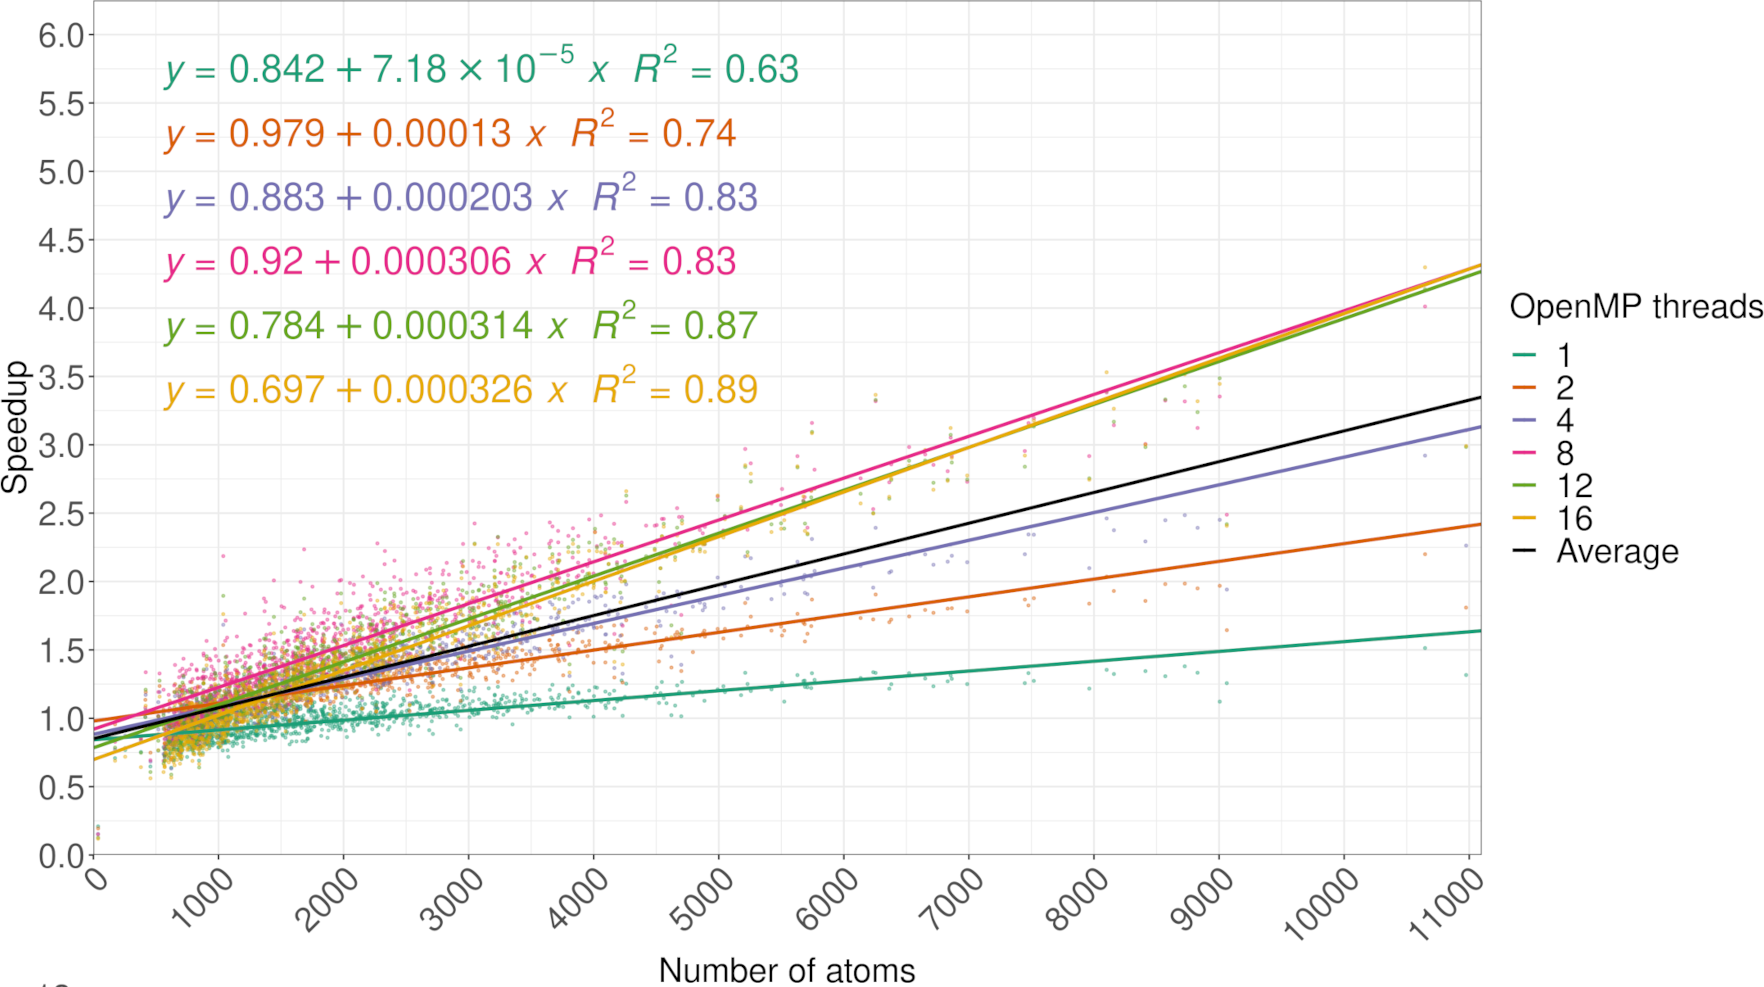
\includegraphics[scale=1]{images/pykvfinder-speedup.png}
  \caption[Ganho de velocidade do pyKVFinder comparado ao parKVFinder]{\textbf{Ganho de velocidade do pyKVFinder comparado ao parKVFinder.} O \textit{speedup} é a razão entre o tempo de execução do pyKVFinder e o tempo de execução do parKVFinder, aplicando o mesmo número de OpenMP \textit{threads}, para diferentes números de átomos.}
  \label{fig:pykvfinder-speedup}
\end{figure}

\subsection{Implementações de novas caracterizações}

Dentro do contexto do pyKVFinder, em colaboração com o Dr. György Szalóki (Laboratoire Hétérochimie Fondamentale et Appliquée - Université Toulouse III Paul Sabatier - França), o escopo do KVFinder suite foi expandido para uma nova classe de moléculas chamadas de gaiolas supramoleculares. Essas gaiolas são moléculas interconectadas que se unem de forma não-covalente, formando uma cavidade interna capaz de encapsular moléculas ou íons. A forma e o tamanho da cavidade são parâmetros importantes que podem ser facilmente determinados por algoritmos geométricos, auxiliando no desenho racional de gaiolas supramoleculares. Nesse contexto, também foram desenvolvidas novas caracterizações aplicáveis tanto para o contexto de gaiolas quanto para biomoléculas.

\subsubsection{Estimativa do volume molecular}

Para a modelagem da superfície molecular, desenvolvemos a classe \textit{Molecule} no pyKVFinder, que permite a modelagem das superfícies moleculares, conforme ilustrado na Figura \ref{fig:surface-representation}, e estimativa do volume molecular, como apresentado na Figura \ref{fig:molecular-modeling}. Nessa abordagem, as moléculas são inseridas em uma grade 3D regular, levando em consideração os raios de vdW de cada um dos átomos da molécula. Os usuários tem a flexibilidade de definir esses raios por meio de um arquivo de configuração (\textit{\href{https://github.com/LBC-LNBio/pyKVFinder/blob/master/pyKVFinder/data/vdw.dat}{vdw.dat}}), assim como a representação de superfície escolhida. Na grade 3D, cada voxel corresponde a um ponto de molécula (0) ou de solvente (1). Portanto, o volume de van der Waals da molécula é estimado somando-se os voxels rotulados como molécula na grade 3D. Essa funcionalidade de estimativa do volume molecular está disponível no pyKVFinder a partir da versão \href{https://github.com/LBC-LNBio/pyKVFinder/tree/v0.5.1}{v0.5.1}. A implementação desses recursos de modelagem e caracterização de moléculas foi detalhada e aplicadas em um artigo publicado no periódico \textit{Journal of Chemical Information and Modeling} \cite{guerra2023B}.

\begin{figure}[ht]
  \centering
  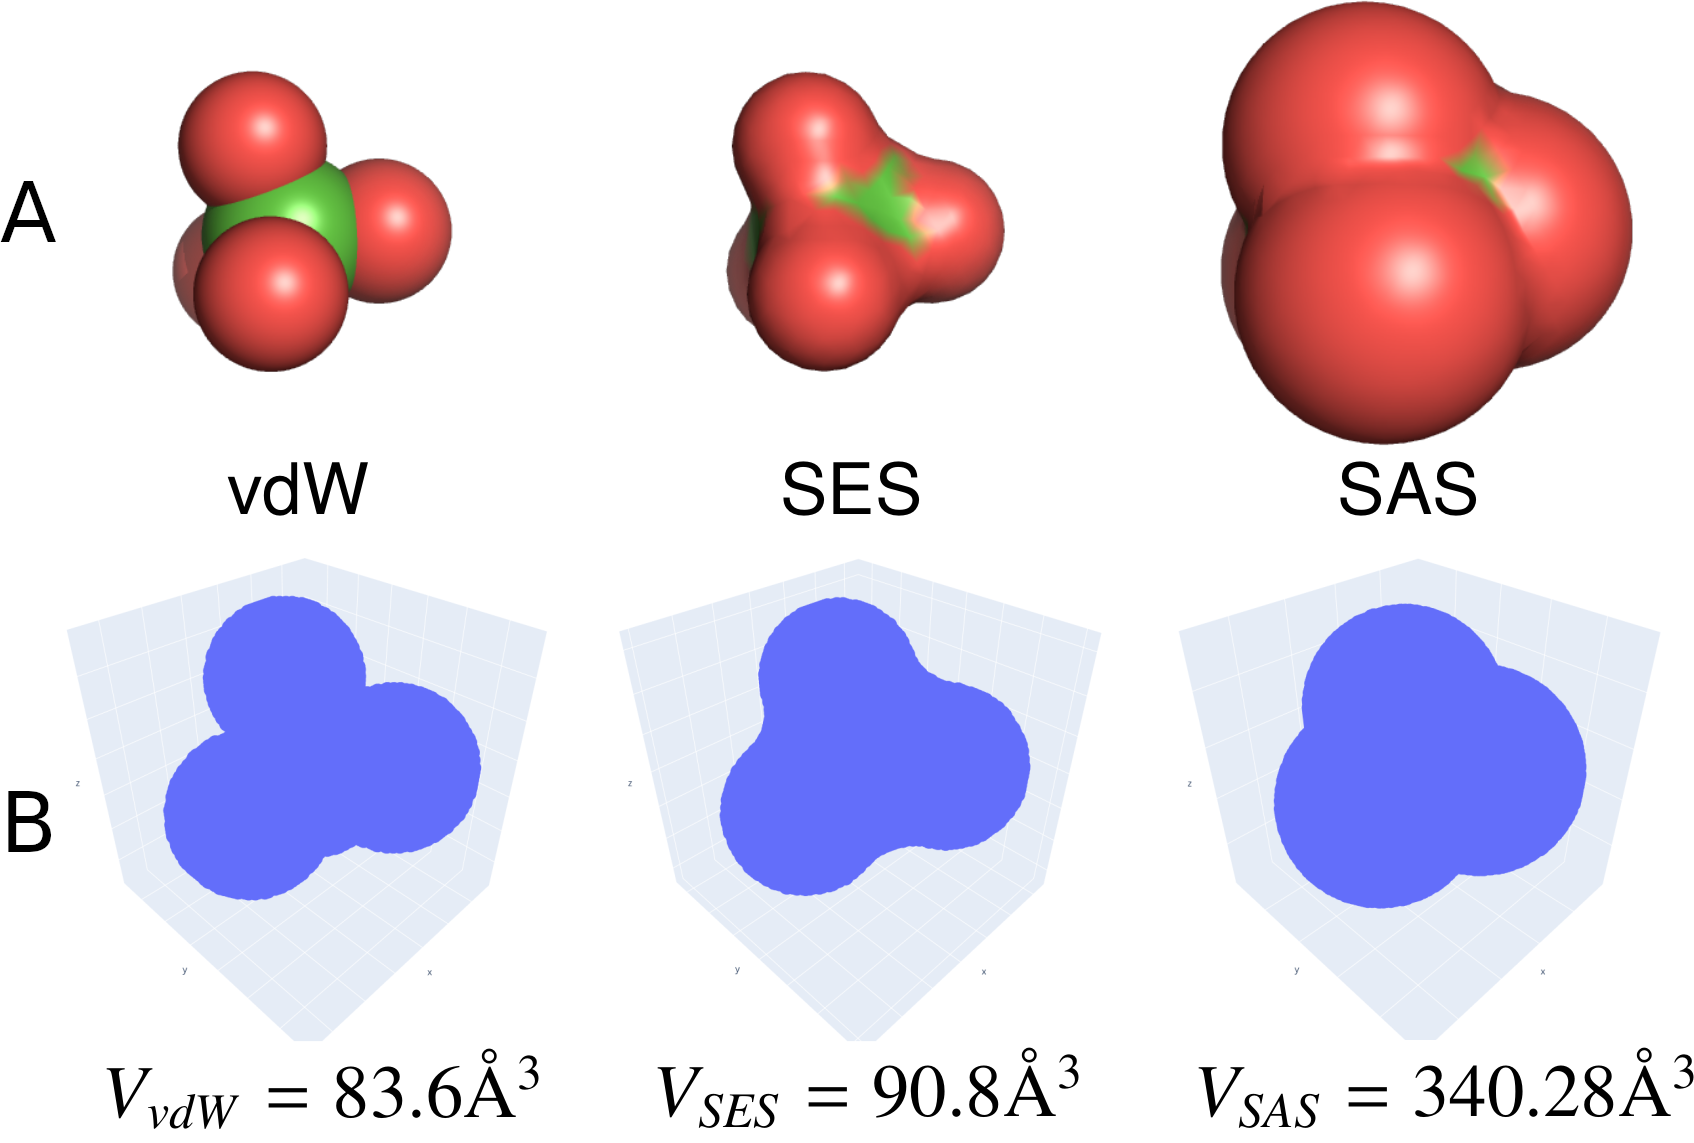
\includegraphics[scale=1.5]{images/molecular-modeling.png}
  \caption[Modelagem e estimativa de volume molecular do perclorato ($ClO_4$)]{\textbf{Modelagem e estimativa de volume molecular do perclorato ($ClO_4$).} \textbf{(A)} Superfície molecular de vdW (quadro esquerdo), SES (quadro central) e SAS (quadro direito) no visualizador molecular PyMOL. \textbf{(B)} Modelagem e estimativa do volume molecular de vdW (quadro esquerdo), SES (quadro central) e SAS (quadro direito) pelo pyKVFinder.}
  \label{fig:molecular-modeling}
\end{figure}

\subsubsection{Caracterização de aberturas}

A compreensão das características das gaiolas supramoleculares, como volume (Figura \ref{fig:cage-characterization}A) e abertura (Figura \ref{fig:cage-characterization}B), que impulsionam o encapsulamento de intermediários reativos é fundamental para o desenho racional de novas gaiolas supramoleculares com propriedades catalíticas aprimoradas. Nesse sentido, desenvolvemos uma caracterização de abertura utilizando o pyKVFinder, que permite a identificação das aberturas, a determinação da área dessas aberturas e a maior sonda esférica (\ie, átomo) que pode passar por cada abertura, conforme ilustrado na Figura \ref{fig:cage-characterization}. 

\begin{figure}[htb]
  \centering
  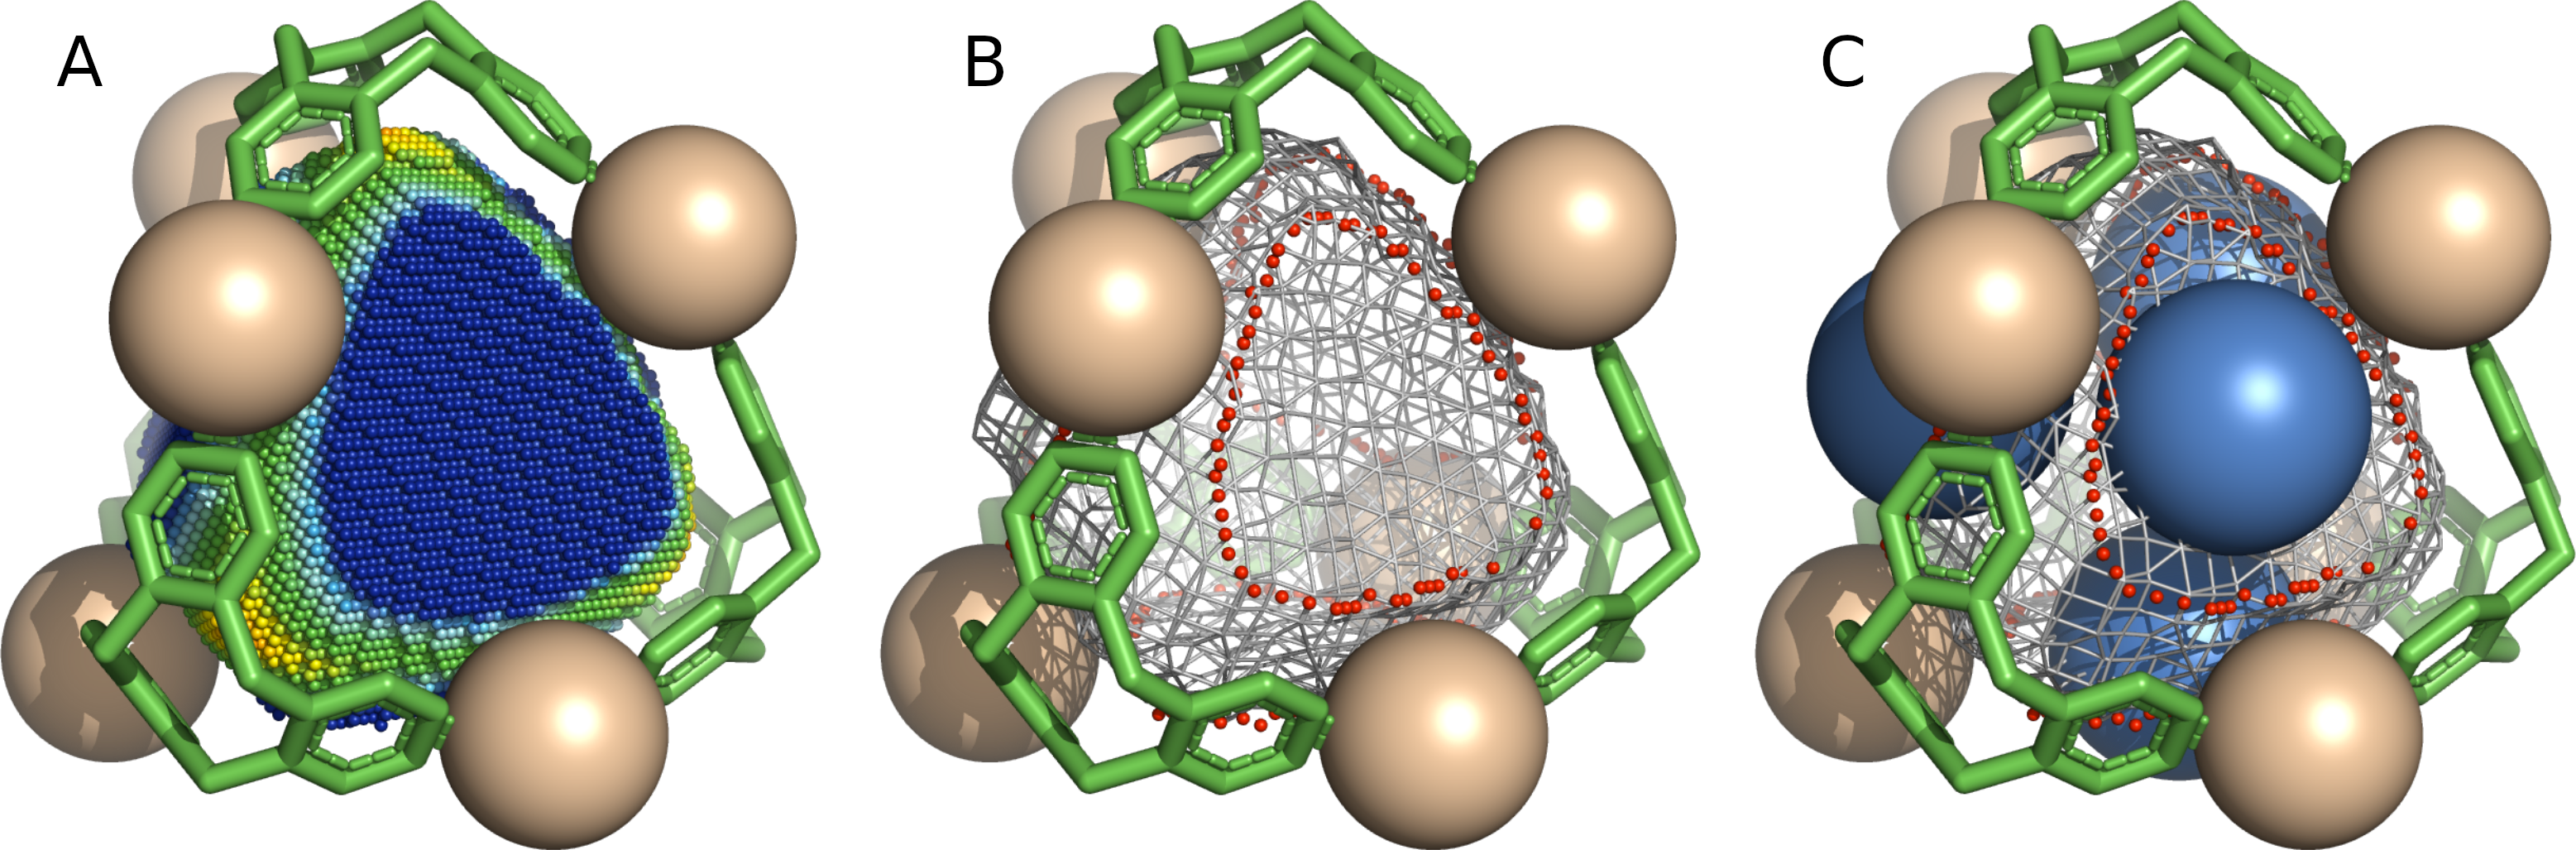
\includegraphics[scale=1.1]{images/cage-characterization.png}
  \caption[Caracterizações de gaiolas supramoleculares]{\textbf{Caracterizações de gaiolas supramoleculares.} \textbf{(A)} Volume e profundidade. Os pontos são coloridos de acordo a profundidade, sendo azul para menor profundidade e vermelho para maior profundidade. \textbf{(B)} Abertura (pontos vermelhos) e área da abertura. \textbf{(C)} Maior sonda esférica (esfera azul) acessível à cavidade da gaiola.}
  \label{fig:cage-characterization}
\end{figure}

O sistema de dupla sonda utiliza identificadores inteiros para os pontos de cavidade (1), pontos de biomolécula (0) e pontos de meio (-1). Após a agrupamento dos pontos de cavidade pelo algoritmo \textit{Depth-First Search} (DFS), os pontos de cavidade são marcados com valores >2, e os pontos de cavidades que não atingiram o volume de corte (parâmetro \textit{volume cutoff}) são mantidos com o valor 1. Nessa abordagem, os pontos de cavidade localizados a uma unidade de grade de um ponto de meio, seguindo a relação do elemento estruturante de \textit{rank} 3 e conectividade 1 (Figura \ref{fig:elementos-estruturantes}), são identificados como pontos de fronteira cavidade-meio, que são marcados com o valor negativo do identificador numérico da cavidade correspondente, conforme descrito para o cálculo de profundidade \cite{guerra2019,guerra2021}. A partir desses pontos de fronteira, é calculada a área superficial utilizando o procedimento de estimativa de área da plataforma KVFinder suite \cite{guerra2019,guerra2020}, que é equivalente à área da abertura. Em seguida, os pontos de fronteira cavidade-meio localizados a uma unidade de grade de um ponto de biomolécula, seguindo a relação do elemento estruturante de \textit{rank} 3 e conectividade 1 (Figura \ref{fig:elementos-estruturantes}), são identificados como pontos de abertura. Nesse estágio, uma nova grade 3D é gerada para acumular os pontos de abertura, que são marcados com o valor 1, enquanto os demais pontos recebem o valor 0. Após o agrupamento dos pontos de abertura pelo algoritmo DFS, os pontos de abertura são marcados com valores >2 (Figura \ref{fig:cage-characterization}B), e aberturas com menos pontos do que um corte definido pelo usuário são marcadas com o valor 1. Por fim, para cada abertura identificada, é calculado o ponto médio e a maior esfera é determinada a partir desse ponto médio, definindo assim o maior átomo que pode passar por essa abertura (Figura \ref{fig:cage-characterization}C).

\subsection{Casos de estudo}

O pyKVFinder foi aplicado em dois casos de estudo publicados em periódicos científicos para investigar proteínas de interesse terapêutico. Essas análises exploraram as características de cavidades de proteínas homólogas ao domínio ADRP do SARS-CoV-2 e a DM do domínio ADRP do SARS-CoV-2 \cite{guerra2021}. No apêndice \ref{ap:casos-de-estudo-pykvfinder}, descreveremos cada um desses casos de estudo em detalhes.

% A seguir, descreveremos cada um desses casos de estudo em detalhes.

\subsection{Discussão}

Apesar de cada método possuir seu próprio conjunto de caracterizações a serem realizadas nas cavidades detectadas, a estrutura de dados das cavidades só é acessível dentro do ecossistema Python no pyKVFinder, que fornece \textit{ndarrays} e dicionários em Python. Ao fornecer uma estrutura de dados acessível e flexível, o pyKVFinder permite aos usuários desenvolver novas caracterizações de cavidades, além de protocolos de análise baseados nessas estruturas de dados. Por exemplo, em um estudo recente conduzido por \cite{jefferson2023}, foi explorada a área transversal das cavidades em proteínas relacionadas usando o pyKVFinder. Esse estudo demonstrou como as estruturas de dados fornecidas pelo pyKVFinder podem ser utilizadas para aprofundar a exploração das cavidades e descobrir informações relevantes para o desenvolvimento de fármacos e a compreensão das interações moleculares. Além disso, a integração do pyKVFinder com o ecossistema Python amplia as possibilidades de análise e visualização de dados, aproveitando as bibliotecas científicas robustas disponíveis nessa linguagem. Essa integração facilita a implementação de análises avançadas e personalizadas, permitindo aos pesquisadores explorar de forma mais abrangente as propriedades das cavidades biomoleculares e obter \textit{insights} valiosos.

Dessa forma, o pyKVFinder não apenas contribui para o avanço da pesquisa em descoberta e desenho racional de fármacos, mas também fortalece a colaboração e o compartilhamento de conhecimentos na comunidade científica. Ao disponibilizar uma ferramenta acessível, flexível e integrada ao ecossistema Python, o pyKVFinder capacita os pesquisadores a explorar as cavidades biomoleculares de forma mais eficiente e eficaz, impulsionando a descoberta de novos alvos terapêuticos e o desenvolvimento de medicamentos mais eficazes.

\section{KVFinder-web}

Nos últimos anos, serviços web que se comunicam por meio dos protocolos de transferência de hipertexto (HTTP; \textit{HyperText Transfer Protocol}, em inglês) se tornaram cada vez mais populares em ambientes de computação em nuvem. Esses serviços fornecem amplo acesso a recursos de dados e processamento. Vários serviços web foram propostos para a detecção e/ou caracterização de sítios de ligação em biomoléculas. Entre eles, podemos citar o FpocketWeb \cite{fpocketweb}, GHECOM \cite{ghecom}, CaverWeb \cite{caverweb}, MoloVol \cite{molovol} e 3DLigandSite \cite{3dligandsite}. Em comparação com outras ferramentas para detecção de cavidades, o parKVFinder possui um conjunto intuitivo de parâmetros e foi extensivamente testado na literatura quanto às suas capacidades de detecção e computacionais, oferecendo desempenho preciso e robusto com qualquer tipo de cavidade proteica, conforme ilustrado anteriormente \cite{guerra2019,guerra2020}. Embora outros métodos também possam detectar sítios de ligação proteicos, cada um possui seu conjunto específico de caracterizações. O parKVFinder se destaca por combinar caracterizações morfológicas, topológicas e fisico-químicas de sítios de ligação, auxiliando efetivamente os usuários na identificação de cavidades funcionalmente relevantes e no estudo do processo de reconhecimento molecular.

\begin{figure}[h]
  \centering
  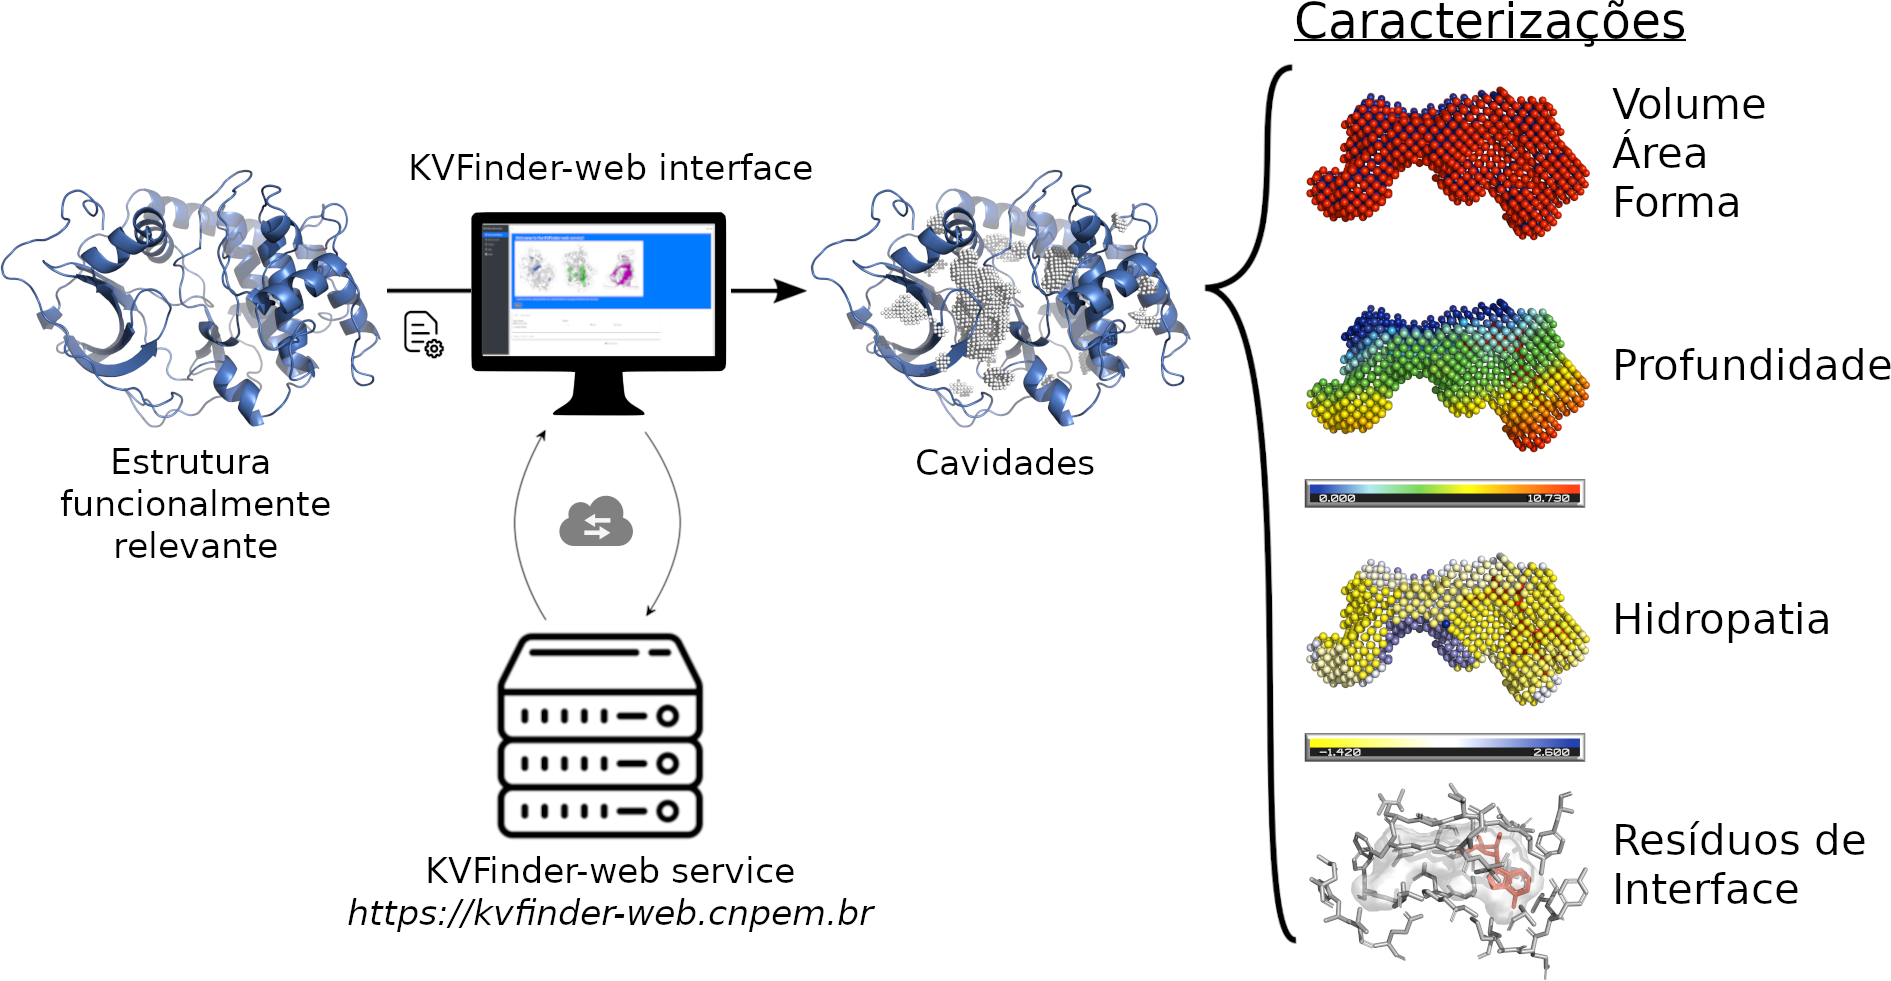
\includegraphics[scale=1.6]{images/kvweb-overview.png}
  \centerline{\scriptsize{\textbf{Fonte:} Adaptado de \cite{guerra2023A}.}}
  \caption[Esquema representativo do funcionamento do KVFinder-web para detectar e caracterizar cavidades em estruturas funcionalmente relevantes]{\textbf{Esquema representativo do funcionamento do KVFinder-web para detectar e caracterizar cavidades em estruturas funcionalmente relevantes.}}
  \label{fig:kvweb-overview}
\end{figure}

Além dos avanços em desempenho e usabilidade do parKVFinder \cite{guerra2019,guerra2020,guerra2023A}, os procedimentos de instalação e configuração da nossa aplicação web, assim como de outras ferramentas independentes para detecção de cavidades, ainda representam uma grande barreira para usuários que não possuem o conhecimento técnico idealmente necessário para executá-los. Além disso, cientistas, educadores e estudantes podem não ter os recursos computacionais locais necessários para os cálculos, o que pode afetar o uso adequado de métodos de detecção e caracterização de cavidades. Nesse cenário, desenvolvemos o \textbf{KVFinder-web}, que foi posteriormente  publicado no periódico \textit{Nucleic Acid Research} \cite{guerra2023A}. O KVFinder-web (Figura \ref{fig:kvweb-overview}), que está disponível em \url{https://kvfinder-web.cnpem.br}, é uma aplicação web de código aberto para detecção e caracterização de cavidades em qualquer tipo de estrutura biomolecular, que consiste em dois componentes independentes: um serviço web RESTful (KVFinder-web service) e uma interface web gráfica (KVFinder-web portal). Para aprimorar ainda mais a experiência do usuário, também fornecemos um plugin gráfico para o PyMOL (PyMOL KVFinder-web Tools).

\subsection{KVFinder-web portal}

O \textbf{KVFinder-web portal} (Figura \ref{fig:kvweb-interface}) é uma interface gráfica interativa do KVFinder-web que oferece aos usuários, especialmente os inexperientes, uma aplicação fácil de usar para executar o parKVFinder (v1.2.0) e analisar os resultados por meio de qualquer navegador. Desenvolvido em R Shiny, o KVFinder-web portal fornece um protocolo simples, direto, robusto e interativo para análise e visualização de cavidades, exigindo apenas uma biomolécula no formato PDB ou o código PDB. Atualmente, o KVFinder-web portal está na versão \href{https://github.com/LBC-LNBio/KVFinder-web-portal/tree/v1.1.0}{v1.1.0}. O código-fonte do KVFinder-web portal está disponível no seguinte repositório: \url{https://github.com/LBC-LNBio/KVFinder-web-portal}.

A interface oferece as principais funcionalidades do KVFinder-web service, permitindo que os usuários carreguem uma biomolécula-alvo a partir de um arquivo PDB ou fornecer o código PDB correspondente, e personalizem os parâmetros de detecção de cavidades e os modos de execução (Figura \ref{fig:kvweb-interface}B). Quatro modos de detecção de cavidades estão disponíveis, oferecendo opções que se adequam melhor à análise da cavidade pelos usuários:

\begin{itemize}
  \item \textit{Whole structure (default)}: detecção de cavidades em toda a estrutura biomolecular com parâmetros de detecção pré-definidos;
  \item \textit{Whole structure (customized)}: detecção de cavidades em toda a estrutura biomolecular com parâmetros de detecção personalizáveis;
  \item \textit{Around target molecule}: detecção de cavidades dentro de um raio ao redor de cada átomo de um ligante ou molécula na estrutura biomolecular-alvo com parâmetros de detecção personalizáveis;
  \item \textit{Around target residues}: detecção de cavidades dentro de uma caixa personalizada, desenhada selecionando resíduos da estrutura biomolecular-alvo e margem da caixa.
\end{itemize}

\begin{figure}[H]
  \centering
  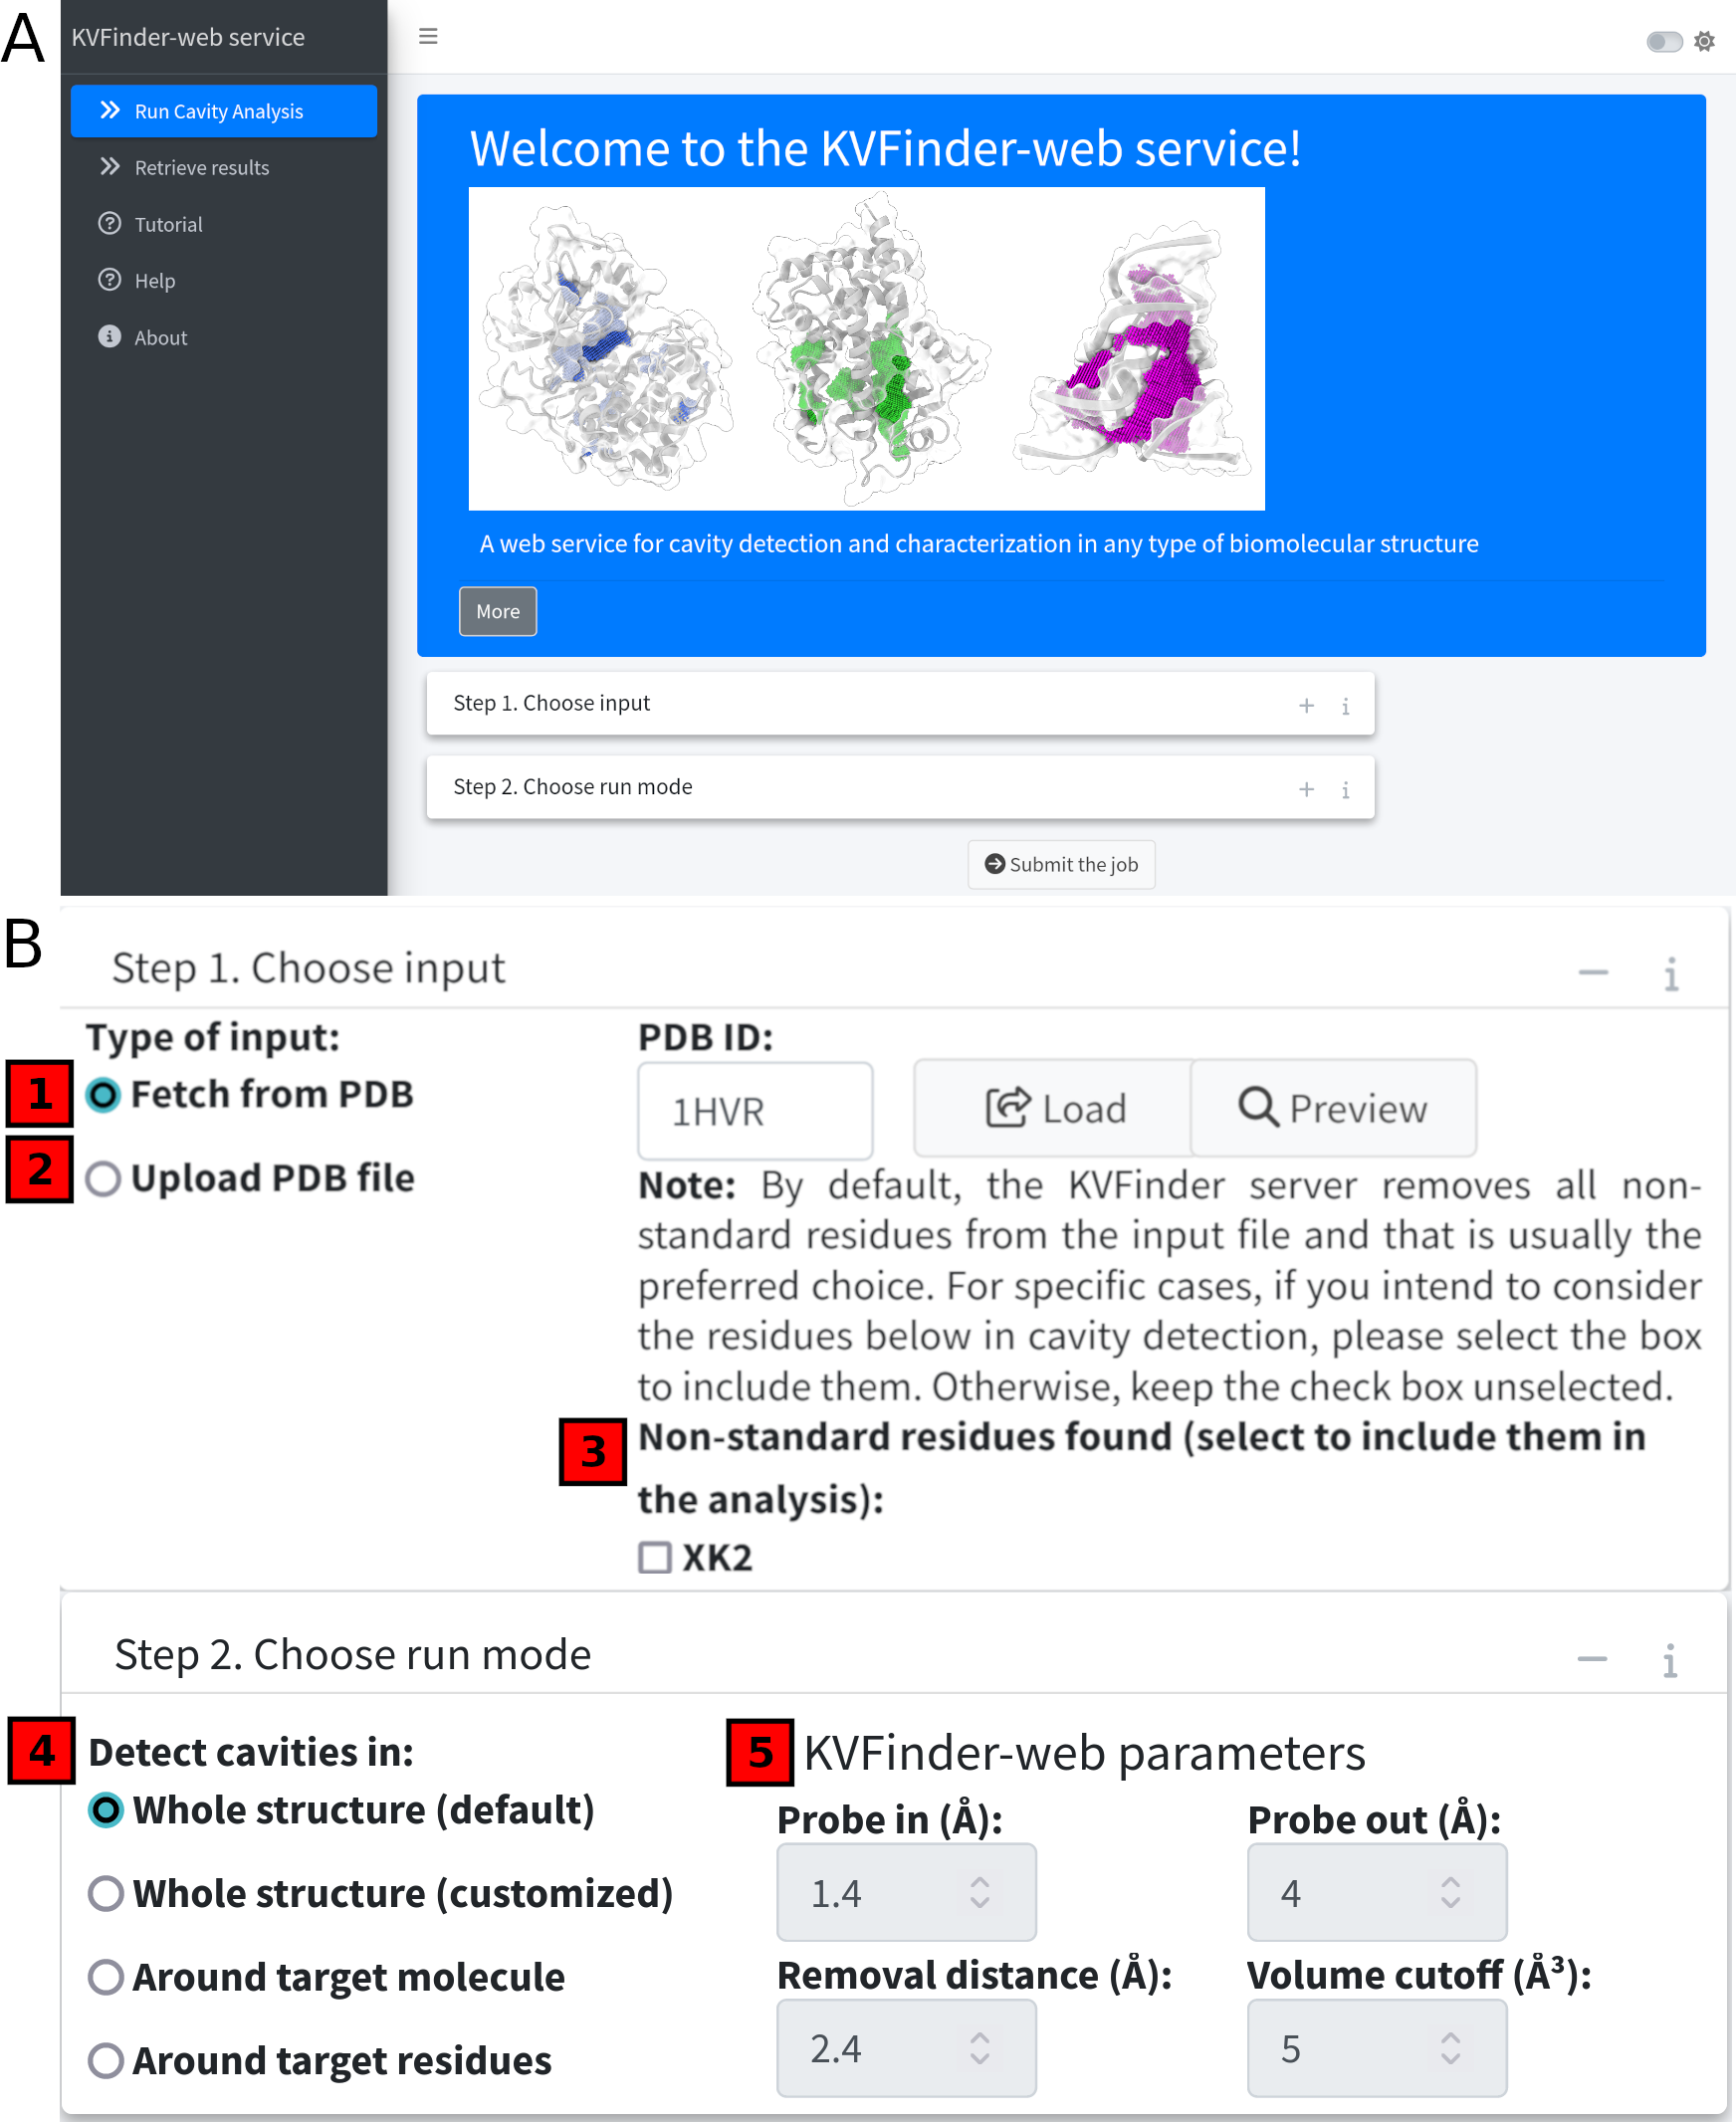
\includegraphics[scale=1.2]{images/kvweb-interface.png}
  \centerline{\scriptsize{\textbf{Fonte:} Adaptado de \cite{guerra2023A}.}}
  \caption[KVFinder-web portal]{\textbf{KVFinder-web portal.} \textbf{(A)} Página principal com as principais abas e as seções de entrada da biomolécula-alvo e escolha do modo de execução. \textbf{(B)} Visão detalhada de cada etapa que os usuários devem concluir antes de enviar a biomolécula-alvo para a análise da cavidade. A primeira etapa envolve a seleção da biomolécula-alvo, que pode ser feita fornecendo um ID do PDB e buscando no banco de dados do PDB (1) ou fazendo o upload de um arquivo PDB (2). Após o upload do PDB, o portal KVFinder-web verifica o PDB e informa sobre resíduos não padronizados detectados (3). Na próxima etapa, os usuários devem selecionar um modo de execução adequado (4) e personalizar, se necessário, os parâmetros de detecção (5).}
  \label{fig:kvweb-interface}
\end{figure}

Os parâmetros personalizáveis de detecção incluem o \textit{Probe In}, o \textit{Probe Out}, o \textit{Removal Distance} e o \textit{Volume Cutoff} (Figura \ref{fig:kvweb-interface}B). Resumidamente, o \textit{Probe In} é uma sonda menor (em$\mAA$) que percorre a biomolécula-alvo, definindo sua superfície molecular (geralmente definida como uma esfera do tamanho de uma molécula de água - $1,4 \mAA$), enquanto o \textit{Probe Out} é uma sonda maior (em$\mAA$) que percorre a biomolécula-alvo, definindo regiões de inacessibilidade. Assim, as cavidades são definidas como as regiões acessíveis ao \textit{Probe In}, que normalmente são mais inclusivas, mas não ao \textit{Probe Out}. A \textit{Removal Distance} é uma distância (em$\mAA$) para remoção de pontos de cavidade a partir da fronteira cavidade-meio, a fim de delimitar os limites externos da cavidade. O \textit{Volume Cutoff} é um filtro de volume da cavidade (em$\mAA^3$) para excluir cavidades com volumes menores que esse limite, geralmente consideradas como cavidades sem relevância funcional. Para obter uma explicação mais detalhada de cada parâmetro, consulte as referências \cite{oliveira2014,guerra2019,guerra2020,guerra2021,guerra2023A}.
 
Além disso, a interface gráfica permite aos usuários baixar e visualizar resultados de uma maneira fácil e interativa (Figura \ref{fig:kvweb-results}). As caracterizações morfológicas (volume, área e profundidade) e físico-químicas (hidrofobicidade) de cada cavidade são mostradas em uma tabela interativa, disponível para download no formato TOML. Um visualizador de biomoléculas, alimentado pelo motor gráfico NGL para R (NGLVieweR \cite{nglviewerr}), exibe a estrutura biomolecular com suas cavidades, para download no formato PDB, e permite várias personalizações, por exemplo, realçar cavidades e exibir resíduos de interface ao redor delas.

\begin{figure}[h]
  \centering
  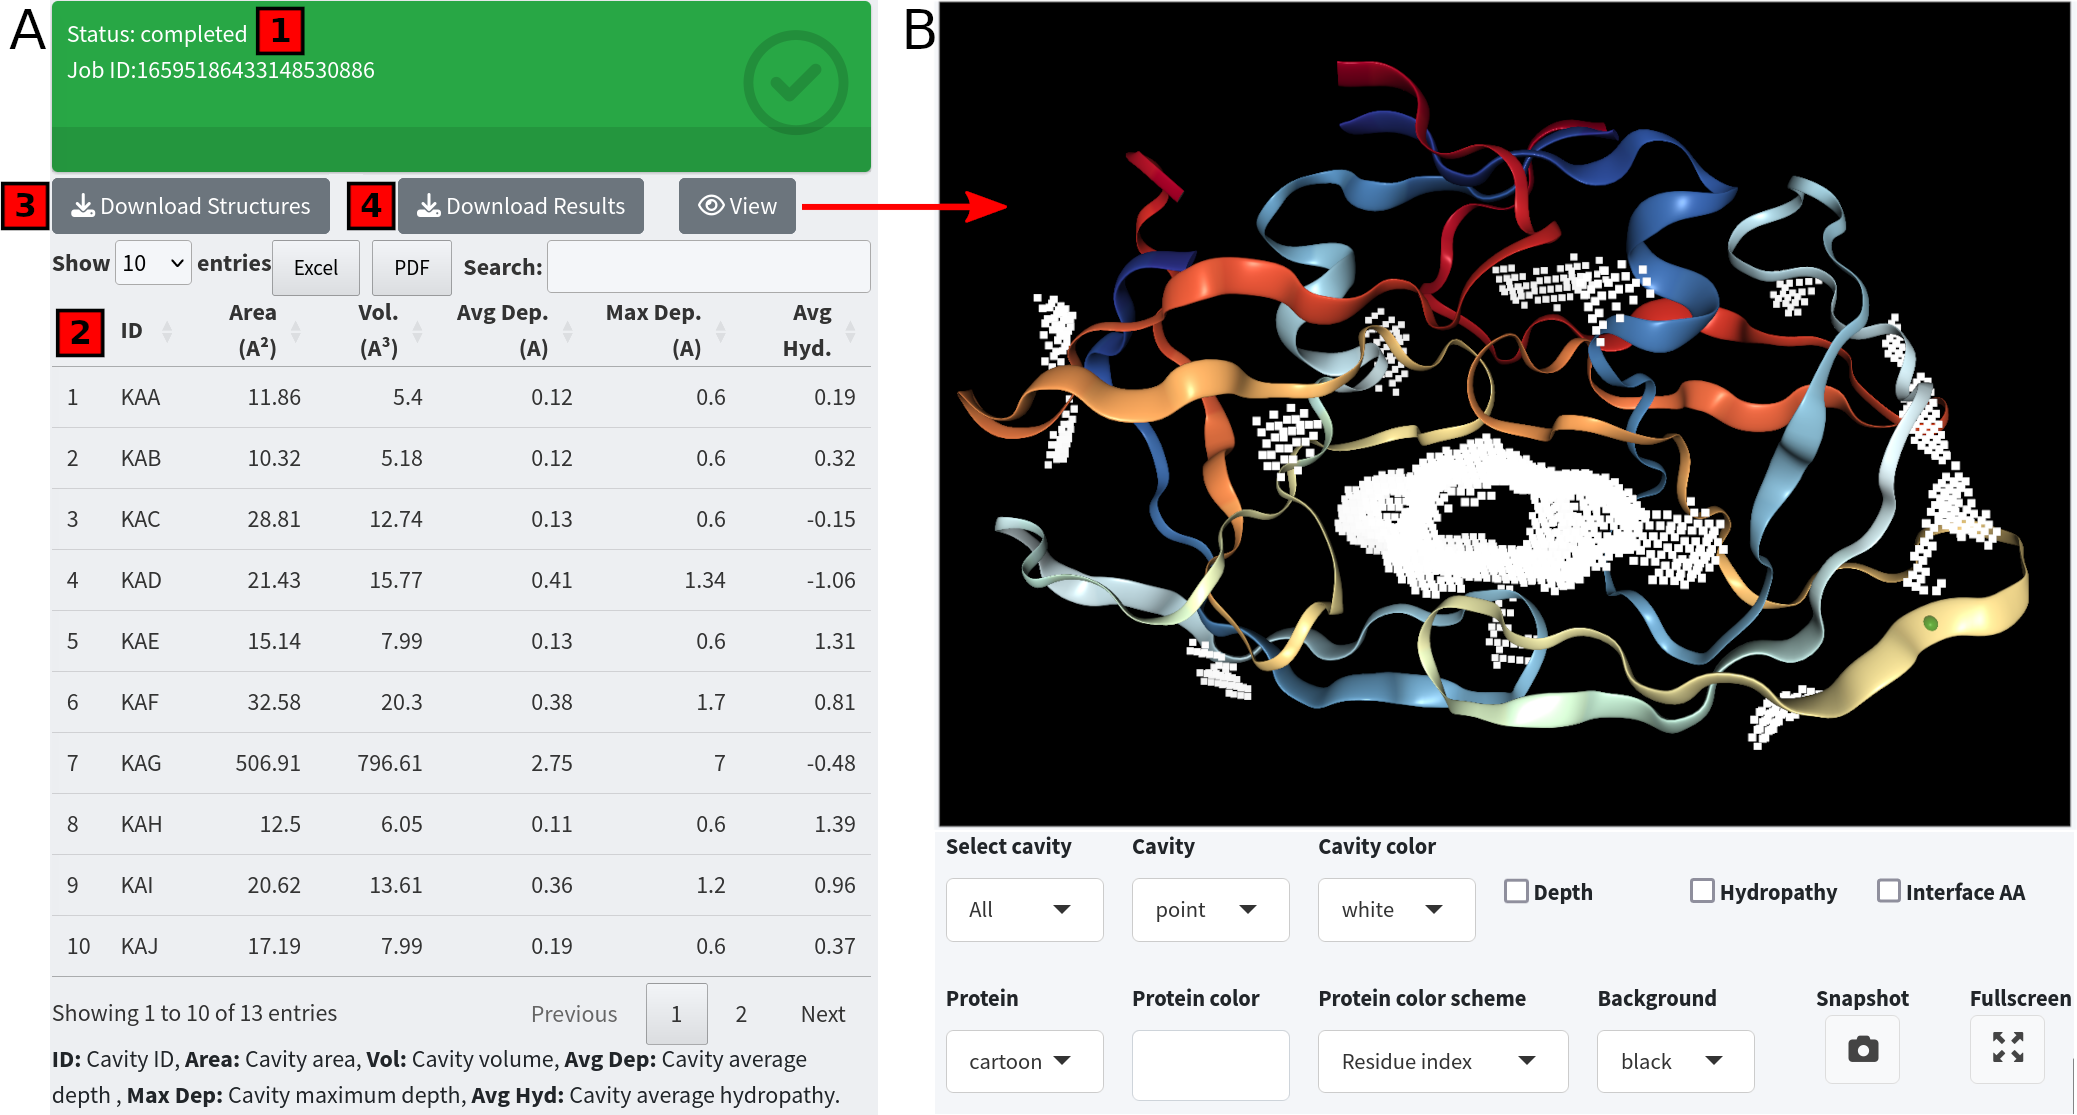
\includegraphics[scale=1.8]{images/kvweb-results.png}
  \centerline{\scriptsize{\textbf{Fonte:} Adaptado de \cite{guerra2023A}.}}
  \caption[Visualização de resultados no KVFinder-web portal]{\textbf{Visualização de resultados no KVFinder-web portal.} \textbf{(A)} Seção de resultados do KVFinder-web portal. A caixa de estado (verde: 'concluído'; amarelo: 'em execução' ou 'em fila'; vermelho: 'cancelado') do trabalho enviado (1). Após a conclusão, a interface apresenta os resultados em uma tabela, incluindo volume, área, profundidade média, profundidade máxima e hidropatia média das cavidades (2). Os usuários podem baixar um arquivo ZIP contendo a biomolécula-alvo e os arquivos PDB das cavidades (3) ou um arquivo TOML com a caracterização das cavidades (4). \textbf{(B)} A biomolécula-alvo com as cavidades pode ser visualizada ao clicar no botão 'Visualizar' e os usuários podem personalizar a visualização da biomolécula e das cavidades.}
  \label{fig:kvweb-results}
\end{figure}

\subsection{KVFinder-web service}

O \textbf{KVFinder-web service} é um serviço web RESTful que utiliza o parKVFinder (v1.2.0) para detectar e caracterizar cavidades em estruturas biomoleculares, conforme descrito em \cite{guerra2019,guerra2020,guerra2023A}. O serviço possui uma arquitetura Web-Fila-Trabalho (\textit{Web-Queue-Worker}, em inglês), que processa solicitações e respostas HTTP da interface web, gerencia os trabalhos e executa o parKVFinder nos trabalhos aceitos. A versão atual do KVFinder-web service é a \href{https://github.com/LBC-LNBio/KVFinder-web-service/tree/v1.1.0}{v1.1.0}. O código-fonte do KVFinder-web service está disponível no repositório: \url{https://github.com/LBC-LNBio/KVFinder-web-service}.

\begin{figure}[H]
  \centering
  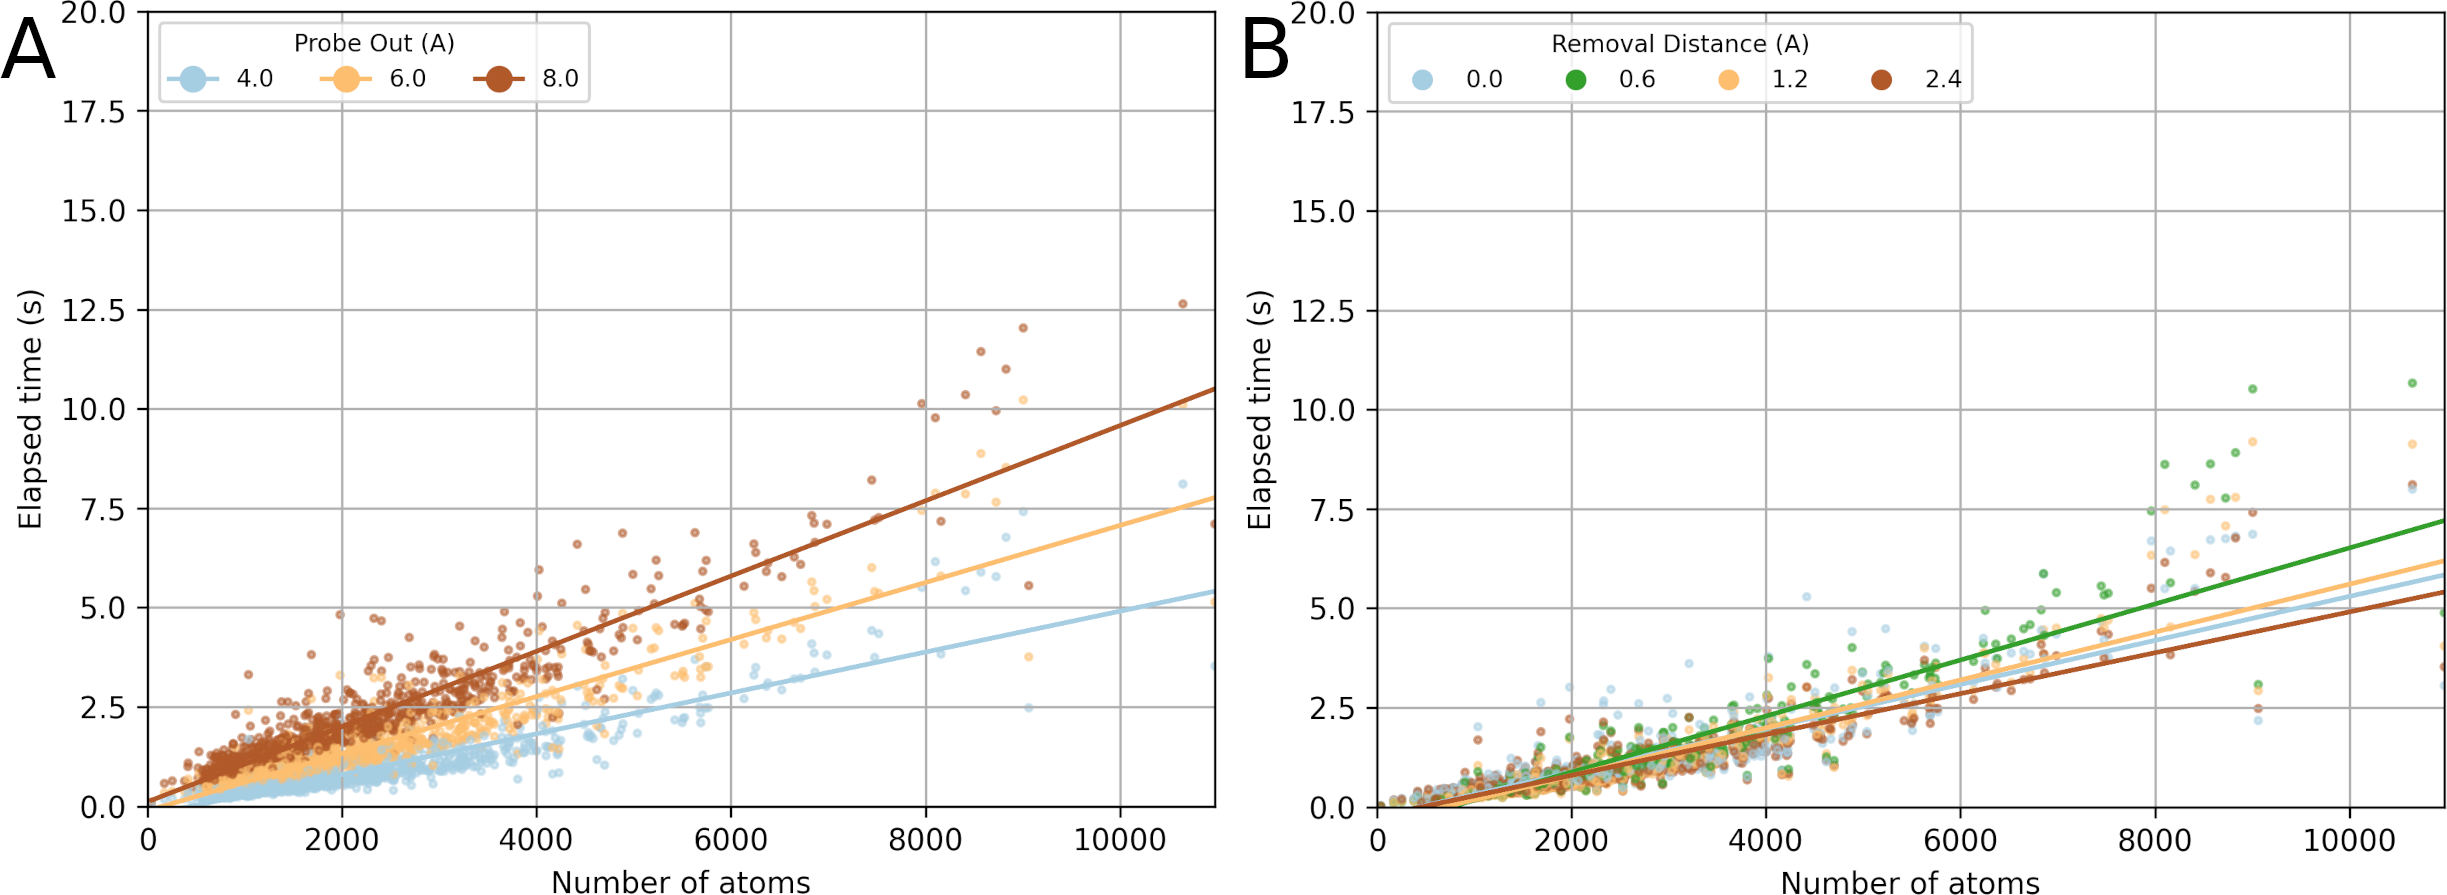
\includegraphics[scale=1.5]{images/kvweb-performance.png}
  \centerline{\scriptsize{\textbf{Fonte:} Adaptado de \cite{guerra2023A}.}}
  \caption[Efeitos dos parâmetros de detecção no desempenho do KVFinder-web service]{\textbf{Efeitos dos parâmetros de detecção no desempenho do KVFinder-web service.} A detecção de cavidades foi realizada no kv1000 \cite{guerra2020}, variando os parâmetros \textit{Probe Out} e \textit{Removal Distance}. O tempo decorrido em relação ao número de átomos na estrutura-alvo foi registrado, variando \textbf{(A)} os tamanhos do \textit{Probe Out} e \textbf{(B)} a \textit{Removal Distance}. Os cálculos foram realizados em um computador com processador AMD Ryzen 7 1700 de 8 núcleos e 3,0 GHz, 32GB de RAM, executando o sistema operacional Ubuntu 22.04 LTS.}
  \label{fig:kvweb-performance}
\end{figure}

O KVFinder-web service utiliza uma arquitetura composta por três módulos: o \textit{Web server}, o \textit{Queue} e o \textit{Worker}. O módulo \textit{Web server}, desenvolvido em Rust usando o framework Actix (\url{https://actix.rs}), recebe as solicitações de trabalho no formato JSON via HTTP POST. Os dados recebidos devem conter as estruturas moleculares e os parâmetros de detecção do parKVFinder. Os trabalhos aceitos pelo módulo \textit{Web server} são enviados para o módulo \textit{Queue}, que é uma instância do servidor de fila de trabalhos Ocypod (\url{https://github.com/davechallis/ocypod}), onde aguardam para serem processados por um módulo \textit{Worker}. O módulo \textit{Worker} se comunica com o módulo \textit{Queue} e solicita o próximo trabalho a ser processado pelo parKVFinder. Após a conclusão do trabalho, a análise da cavidade (cavidades e suas caracterizações) é enviada de volta ao módulo \textit{Queue}, atualizando o status e os resultados do trabalho, que são disponibilizados aos clientes por meio do módulo \textit{Web server}. Para recuperar os resultados do trabalho, o cliente envia uma solicitação HTTP GET com o ID do trabalho, e o servidor web retorna o status atual do trabalho - 'em fila', 'em execução' ou 'concluído' - juntamente com os respectivos resultados, se disponíveis. Cada trabalho permanece armazenado em cache na fila por um dia após a conclusão. Como o ID do trabalho é criado aplicando uma função \textit{hash} nos dados recebidos, os resultados em cache são retornados quando a solicitação é reenviada. Cada módulo do KVFinder-web service é empacotado em um contêiner Docker \cite{docker}, tornando-o disponível para execução em ambientes locais ou de computação em nuvem. Esses módulos são combinados em um arquivo Docker Compose para facilitar a implantação.

O desempenho computacional do KVFinder-web service também foi avaliado no kv1000 \cite{guerra2020}, variando dois parâmetros importantes relacionados à detecção de cavidades: \textit{Probe Out} e \textit{Removal Distance} (Figura \ref{fig:kvweb-performance}). A variação do parâmetro \textit{Probe Out} cria uma superfície molecular mais espessa ao redor da estrutura biomolecular, definindo a fronteira da cavidade. O aumento do valor do \textit{Probe Out} reduz a acessibilidade da superfície molecular e aumenta o tempo de cálculo no KVFinder-web service. Já o parâmetro \textit{Removal Distance} remove pontos da cavidade que estão próximos à fronteira, auxiliando na identificação de subcavidades e cavidades superficiais. O tempo de execução não apresenta uma relação clara com o parâmetro \textit{Removal Distance}, pois é influenciado pelo tamanho da fronteira e pelo número de cavidades, e não pelo número de átomos. De maneira geral, o tempo de execução aumenta de forma linear com o número de átomos na biomolécula-alvo dentro da grade 3D.

\subsection{PyMOL KVFinder-web Tools}

Para usuários familiarizados com o PyMOL \cite{pymol}, a ferramenta \textbf{PyMOL KVFinder-web Tools} (Figura \ref{fig:pymol-kvweb-tools}), desenvolvida em Python3 e Qt, integra o KVFinder-web service com o programa de visualização molecular. Essa interface gráfica de usuário (GUI; \textit{Graphical User Interface}, em inglês) amigável permite a personalização dos parâmetros de detecção para uma estrutura biomolecular-alvo e envia os trabalhos para um serviço KVFinder-web configurado (Figura \ref{fig:pymol-kvweb-tools}A). Atualmente, o PyMOL KVFinder-web Tools está na versão \href{https://github.com/LBC-LNBio/PyMOL-KVFinder-web-Tools/tree/v1.0.0}{v1.0.0}. O código-fonte do PyMOL KVFinder-web Tools está disponível no seguinte repositório: \url{https://github.com/LBC-LNBio/PyMOL-KVFinder-web-Tools}.

\begin{figure}[H]
  \centering
  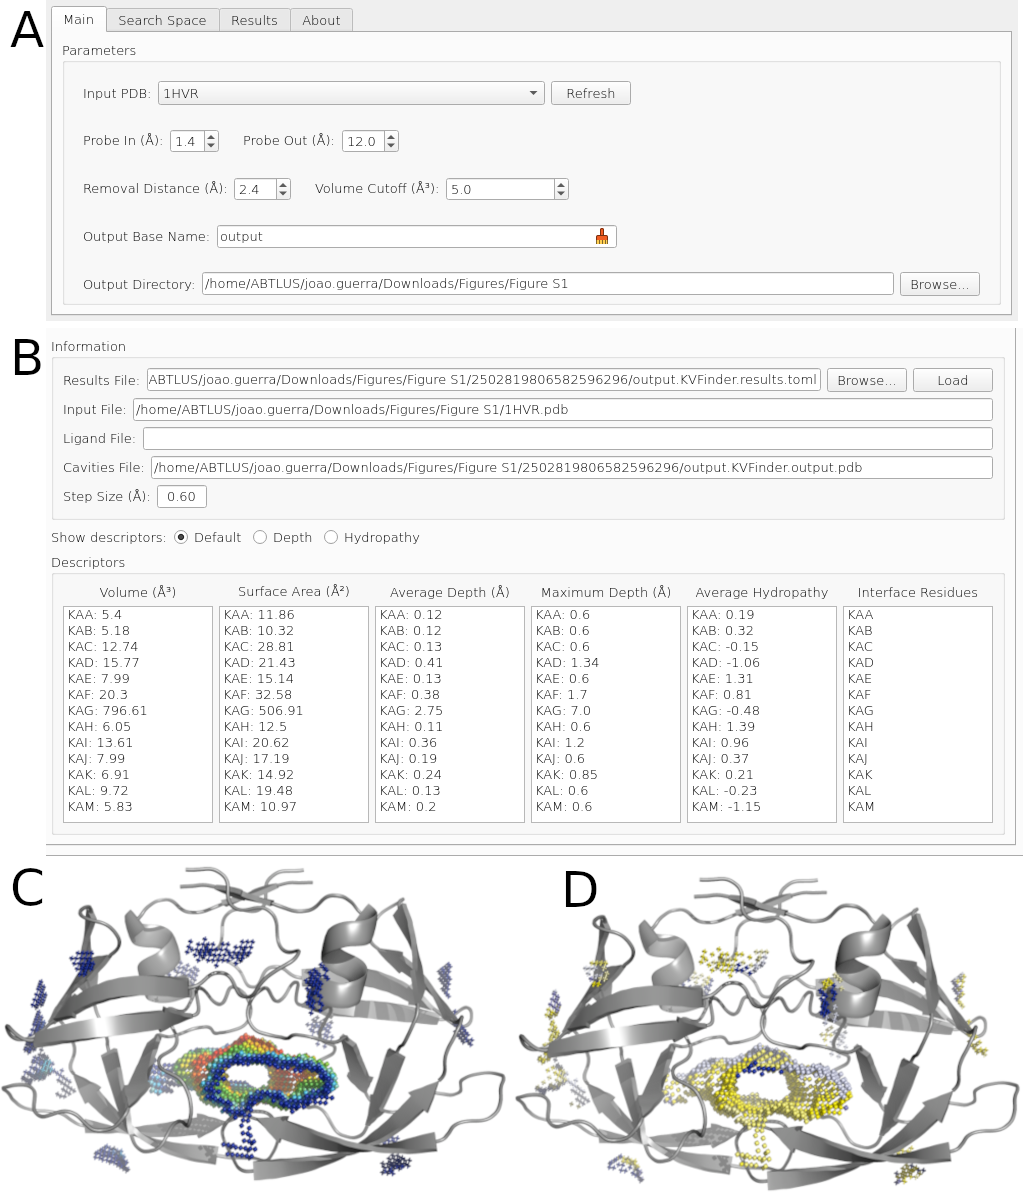
\includegraphics[scale=2.5]{images/pymol-kvweb-tools.png}
  \centerline{\scriptsize{\textbf{Fonte:} Adaptado de \cite{guerra2023A}.}}
  \caption[PyMOL KVFinder-web Tools]{\textbf{PyMOL KVFinder-web Tools.} Detecção de cavidades na estrutura da protease do HIV-1 (PDB ID: 1HVR), com \textit{Probe Out} definido como 12 Å. \textbf{(A)} Aba de parâmetros principais contendo parâmetros de detecção e estruturas moleculares a serem exploradas. \textbf{(B)} Aba de visualização contendo dados recebidos (cavidades e caracterizações) do serviço KVFinder-web exibidos na GUI. \textbf{(C)} Caracterização de profundidade e \textbf{(D)} caracterização de hidropatia de Eisenberg & Weiss, destacando o sítio ativo (cavidade KAG) na GUI e no visualizador do PyMOL.}
  \label{fig:pymol-kvweb-tools}
\end{figure}

Assim como no plugin parKVFinder para PyMOL \cite{guerra2020}, o espaço de busca também pode ser ajustado para uma caixa personalizada (\textit{box adjustment mode}) e/ou um raio ao redor de um ligante ou molécula-alvo (\textit{ligand adjustment mode}), em vez de detectar e caracterizar cavidades em toda a superfície biomolecular (\textit{whole protein mode}). Após o envio bem-sucedido, os trabalhos aceitos são solicitados rotineira e assincronamente ao KVFinder-web service. Quando um trabalho é concluído, o plugin processa automaticamente os dados recebidos, cavidades e caracterizações, para arquivos locais e os disponibiliza na GUI. Esse plugin gráfico opera de maneira semelhante ao KVFinder-web portal, as caracterizações são mostradas em listas (Figura \ref{fig:pymol-kvweb-tools}B) e as cavidades são personalizadas por suas propriedades no visualizador do PyMOL (Figura \ref{fig:pymol-kvweb-tools}C e D). No entanto, os trabalhos enviados no KVFinder-web portal podem ser carregados no PyMOL KVFinder-web Tools e vice-versa.

\subsection{Caso de estudo}

O KVFinder-web foi aplicado em dois casos de estudo publicados em periódico científico para investigar proteínas de interesse terapêutico. Essas análises exploraram a caracterização do sítio catalítico da protease do vírus da imunodeficiência humana tipo 1 (HIV-1) e a comparação morfológica das estruturas desta proteína depositadas no wwPDB. No apêndice \ref{ap:casos-de-estudo-kvfinder-web}, descreveremos cada um desses casos de estudo em detalhes.

\subsection{Discussão}

Em linhas gerais, a disponibilização do KVFinder-web visa ampliar o uso dessa robusta ferramenta de detecção de cavidades na comunidade científica. Além disso, o KVFinder-web tem o propósito de democratizar a ferramenta parKVFinder e remover as barreiras para usuários que não possuem conhecimento técnico para instalar e configurar um ferramenta computacional de detecção de cavidades, que possuem recursos computacionais limitados ou que desejam realizar uma análise simples e rápida. Isso simplificará o processo de detecção e caracterização de cavidades, mesmo para usuários menos experientes, com impacto direto no busca e desenho racional de fármacos e na compreensão das estruturas de biomoléculas.

\section{SERD \label{sec:serd}}

A teoria de grafos tem sido relevante tanto no campo da biologia quanto nas ciências farmacêuticas, sendo aplicada no estudo da estrutura, função e evolução de proteínas, bem como em análises de DM e redes de interação receptor-ligante \cite{vishveshwara2002,mason2007,hummer2023}. Conforme apresentado em \cite{hummer2023}, as representações de complexos proteína-proteína (\ie, complexos anticorpo-antígeno) podem ser aplicadas em técnicas de aprendizado profundo (\textit{deep learning}, em inglês) para prever $\Delta \Delta G$ experimental. Além disso, as representações em forma de grafo podem ser utilizadas em uma ampla gama de técnicas de aprendizado de máquina e ciência de dados, conforme ilustrado na Seção \ref{sec:graph-representation} e discutido em estudos anteriores \cite{majeed2020,vishveshwara2002,mason2007}. Neste cenário, desenvolvemos o \textbf{SERD}, uma ferramenta para representação de estruturas biomoleculares na forma de grafos, desde sítios de ligação (\eg, cavidades identificadas pelo KVFinder suite) até complexos biomoleculares (\eg, IPPs, IPLs, IPRs e IPDs), conforme ilustrado na Figura \ref{fig:serd-graph}. Atualmente, o SERD está na versão \href{https://github.com/jvsguerra/SERD/tree/v0.1.2}{v0.1.2}. O código-fonte do SERD está disponível no seguinte repositório: \url{https://github.com/jvsguerra/SERD}.

Além disso, sabe-se que o reconhecimento molecular depende diretamente da acessibilidade de um ligante ao sítios de ligação do seu respectivo receptor. Os resíduos expostos ao solvente de uma biomolécula-alvo (receptor) compõe o conjunto de átomos acessíveis a possíveis ligantes. Nesse contexto, a identificação desses resíduos possibilita um estudo mais direcionado aos \textit{hotspots} de interação de um receptor-alvo, com aplicações principalmente no estudo de acoplamento molecular (\eg, \textit{docking} proteína-proteína e \textit{docking} proteína-ligante). No SERD, também implementamos um algoritmo para identificar resíduos expostos ao solvente em uma biomolécula-alvo. Essa abordagem aproxima uma molécula de solvente a uma sonda esférica, que escaneia a superfície do receptor alvo para identificar as regiões (\ie, resíduos) que são acessíveis a esta sonda esférica, de forma semelhante ao escaneamento da grade 3D da sonda \textit{Probe Out} no KVFinder suite \ref{fig:kvfinder-suite-schema}. Após a identificação desses resíduos, a ferramenta os representa na forma de grafos pela biblioteca NetworkX \cite{networkx}, formando arestas até uma distância limite entre C\textalpha, C\textbeta\space ou quaisquer átomos do resíduo e opcionalmente incluir essas distâncias como atributos das arestas desses grafos. Opcionalmente, essas distâncias podem ser incluídas como atributos das arestas desses grafos, conforme ilustrado na Figura \ref{fig:serd-graph}B.

Por fim, esta ferramenta é aplicada em duas colaborações do Laboratório de Biologia Computacional: o projeto de Mestrado do aluno Marcos Rogério Simões do PPGCF/FCF, intitulado "Descrição e caracterização de sítios de ligação através de teoria dos grafos", para estudar a similaridade entre sítios de ligação entre famílias de quinases, e o projeto de pesquisa do Dr. Gabriel Ernesto Jara para estudo de complexos anticorpo-antígeno através de fragmentos da superfície.

\section{KVFinderMD}

Em algumas circunstâncias, para a formação do complexo receptor-ligante, os receptores utilizam sítios de ligação que não são facilmente identificados na forma não-ligada. Algumas interações biomoleculares (\eg, IPPs, IPLs, IPRs and IPDs) dependem da dinâmica intrínseca do receptor-alvo, nas quais o modelo clássico de chave-fechadura falha e modelos mais recentes de ligação, como ajuste induzido e seleção conformacional, são aplicáveis \cite{holyoak2013}. Nesse sentido, as simulações de DM são uma ferramenta útil para entender os mecanismos de reconhecimento molecular e, em última análise, a função biomolecular. Recentemente, desenvolvemos o pyKVFinder \cite{guerra2021} como um bloco de construção para aplicações mais complexas, como análises de simulações de DM. Utilizando-o como base, desenvolvemos uma nova ferramenta chamada \textbf{KVFinder for Molecular Dynamics analysis (KVFinderMD)}, um pacote em Python que permite explorar a dinâmica dos sítios de ligação em estruturas biomoleculares de interesse farmacológico. Uma vez que a dinâmica intrínseca da biomolécula pode alterar a forma e as propriedades do sítio de ligação ao longo do tempo, o KVFinderMD caracteriza cavidades em relação ao volume, área, profundidade, hidropatia e resíduos de interface, que são propriedades relevantes para descrever o processo de reconhecimento molecular (Figura \ref{fig:kvmd-overview}A). 

\begin{figure}[h]
  \centering
  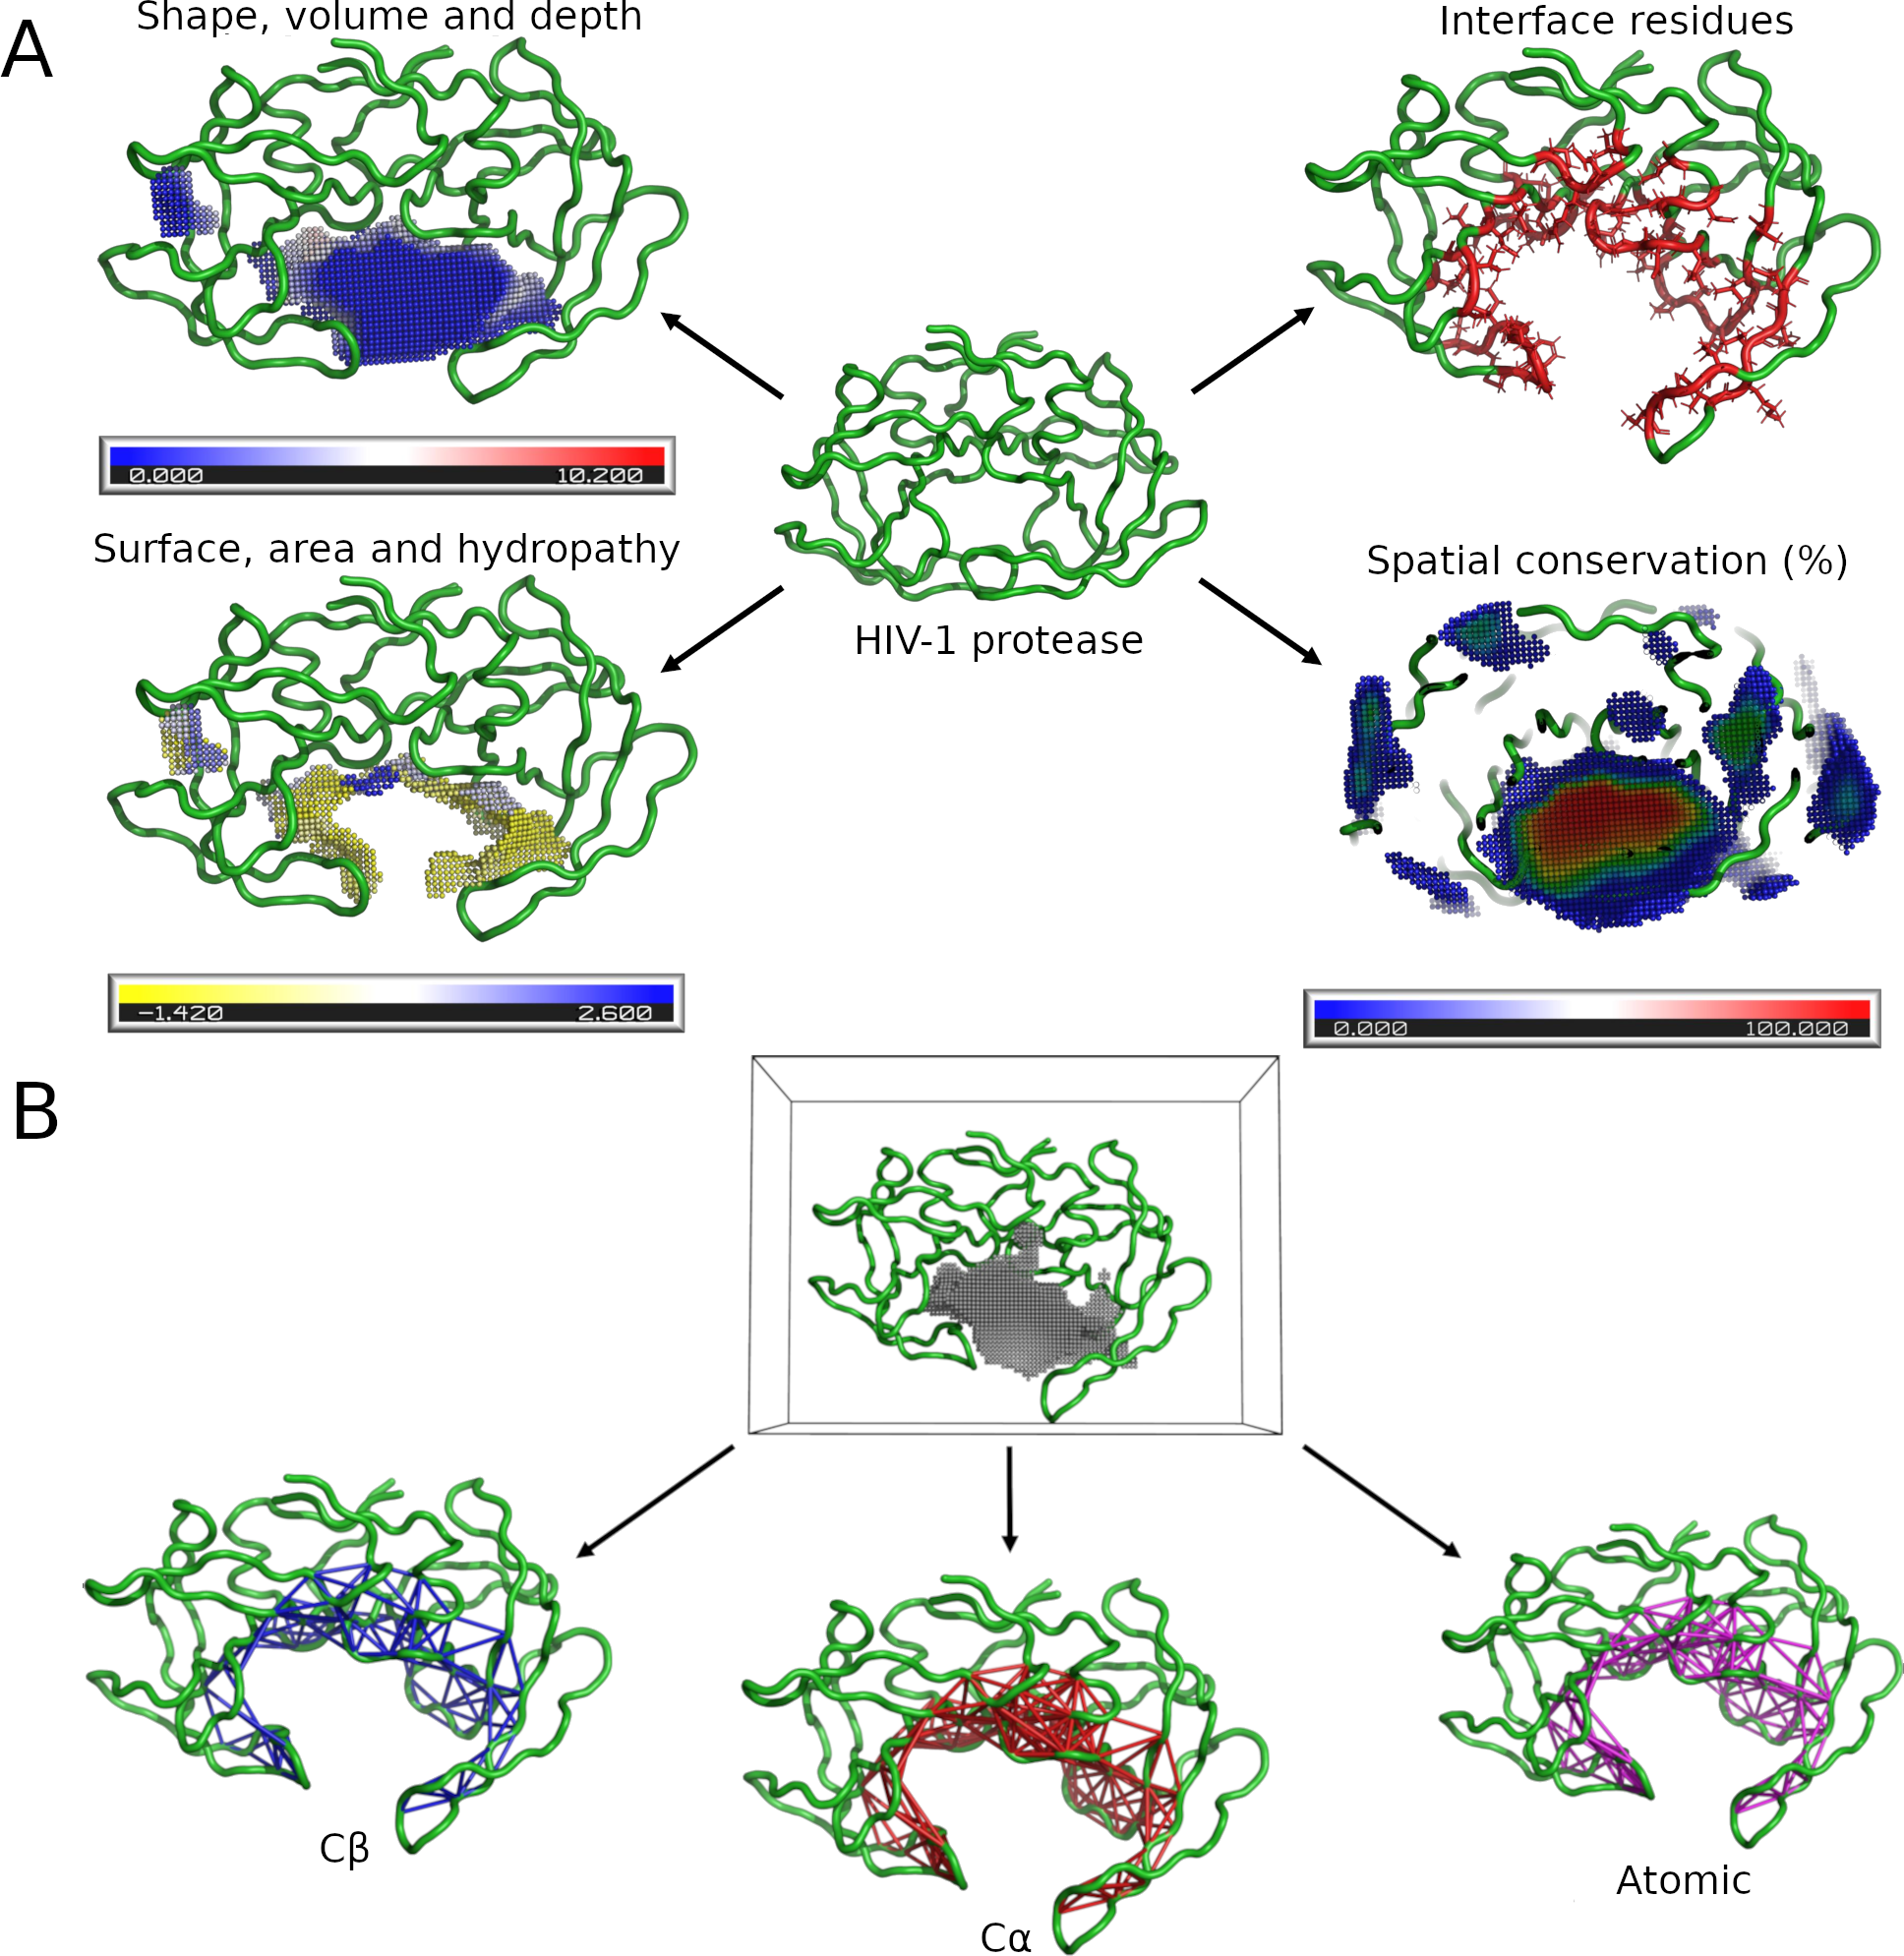
\includegraphics[scale=0.8]{images/kvmd-overview.png}
  \caption[Detecção, caracterizações e representações de cavidades em estudos de dinâmica molecular usando a ferramenta KVFinderMD]{\textbf{Detecção, caracterizações e representações de cavidades em estudos de dinâmica molecular usando a ferramenta KVFinderMD.} \textbf{(A)} Caracterizações morfológicas, topológicas e físico-químicas aplicadas no KVFinderMD. \textbf{(B)} Representação em forma de grafo das cavidades baseada nos resíduos de interface e suas relações topológicas. Distância entre C\textbeta\space(azul), C\textalpha\space(vermelho) e quaisquer átomos de um resíduo (magenta).}
  \label{fig:kvmd-overview}
\end{figure}

Para a leitura de dados binários gerados por programas de simulação de DM, como GROMACS \cite{gromacs}, AMBER \cite{amber} e CafeMol \cite{kenzaki2011}, utilizamos o pacote MDAnalysis \cite{mdanalysis} para integrar a leitura e processamento dos arquivos de trajetória de DM (\eg, GRO, CRD, NC, DCD, XTC/TRR) e os arquivos de topologia (\eg, PSF, PRMTOP, GRO, PDB) no KVFinderMD. Adicionalmente, implementamos um protocolo para a análise de conservação de cavidades ao longo da DM (Figura \ref{fig:kvmd-overview}A; quadro inferior direito), similar ao apresentado na análise de conservação do sítio de ligação do ADP-ribose no domínio ADRP do SARS-CoV-2 e proteínas relacionadas (Figura \ref{fig:conservation-analysis}). Por fim, também integramos a representação em forma de grafos, implementada no SERD (veja Seções \ref{sec:graph-representation} e \ref{sec:serd}), que considera distâncias carbono \textalpha, carbono \textbeta\space ou quaisquer átomos, para descrever o sítio de ligação (Figura \ref{fig:kvmd-overview}B). Desta forma, a similaridade das cavidades pode ser determinada a partir do agrupamento hierárquico das representações de grade 3D, topológica e em forma de grafos das cavidades, permitindo acompanhar as cavidades ao longo da DM.

\subsection{Caso de estudo}

% O KVFinderMD foi aplicado em dois casos de estudo para investigar proteínas de interesse terapêutico. Essas análises exploraram a similaridade de cavidades da protease da HIV-1 ao longo de uma simulação de DM e a caracterização dos sítios de ligação do substrato de ALDH1 e ALDH2. Ambos casos de estudo foram apresentados em detalhe no IV Congresso de Estudantes do CNPEM (IV CEC), realizado entre 22 e 24 de novembro de 2022, e recebeu prêmio pela apresentação intitulada "KVFinderMD: a Python package to detect and describe binding sites in molecular dynamics trajectories".

O KVFinderMD foi aplicado em um caso de estudo para explorar a similaridade de cavidades da protease da HIV-1 ao longo de uma simulação de DM. Este caso de estudo foi apresentado em detalhe no IV Congresso de Estudantes do CNPEM (IV CEC), realizado entre 22 e 24 de novembro de 2022, e recebeu prêmio pela apresentação intitulada "KVFinderMD: a Python package to detect and describe binding sites in molecular dynamics trajectories".

\subsubsection{Similaridade de cavidades da HIV-1 protease ao longo de uma simulação de dinâmica molecular}

Partindo da DM da HIV-1 protease, onde descrevemos com sucesso as alterações conformacionais que definem o sítio ativo (veja Seção \ref{sec:md-hiv1-protease}), aplicamos um alinhamento estrutural das cavidades, usando representações em grade 3D, representação topológica e representação em grafos, da protease do HIV-1 ao longo da simulação de DM. Com as três representações de cavidades implementadas no KVFinder suite, exploramos algoritmos de agrupamento não-supervisionados, onde o agrupamento hierárquico apresentou os melhores resultados, além de fornecer uma relação de similaridade entre as cavidades. Além disso, exploramos diferentes métricas de afinidade para agrupar as cavidades ao longo da trajetória da HIV-1 protease.

Para realizar o agrupamento, separamos cada cavidade em uma estrutura de dados individual e adaptamos a codificação dos dados de sítios de ligação (Figura \ref{fig:hiv-1-representation}). Na representação de grade 3D, transformamos os valores armazenados em booleanos, onde os pontos de cavidades são marcados com o valor 1, enquanto os demais pontos recebem o valor 0. Na representação topológica, transformamos os valores em uma matriz quadrada de distâncias entre os resíduos, ordenados de acordo com a sequência da proteína. Por fim, na representação em grafo, transformamos os valores em uma matriz quadrada de contatos entre os resíduos, também ordenados de acordo com a sequência da proteína. Para isso, utilizamos a distância entre os átomos de C\textbeta\space dos resíduos, com o corte de distância de 8 \AA para definir os contatos, que é a métrica padrão do SERD.

\begin{figure}[h]
  \centering
  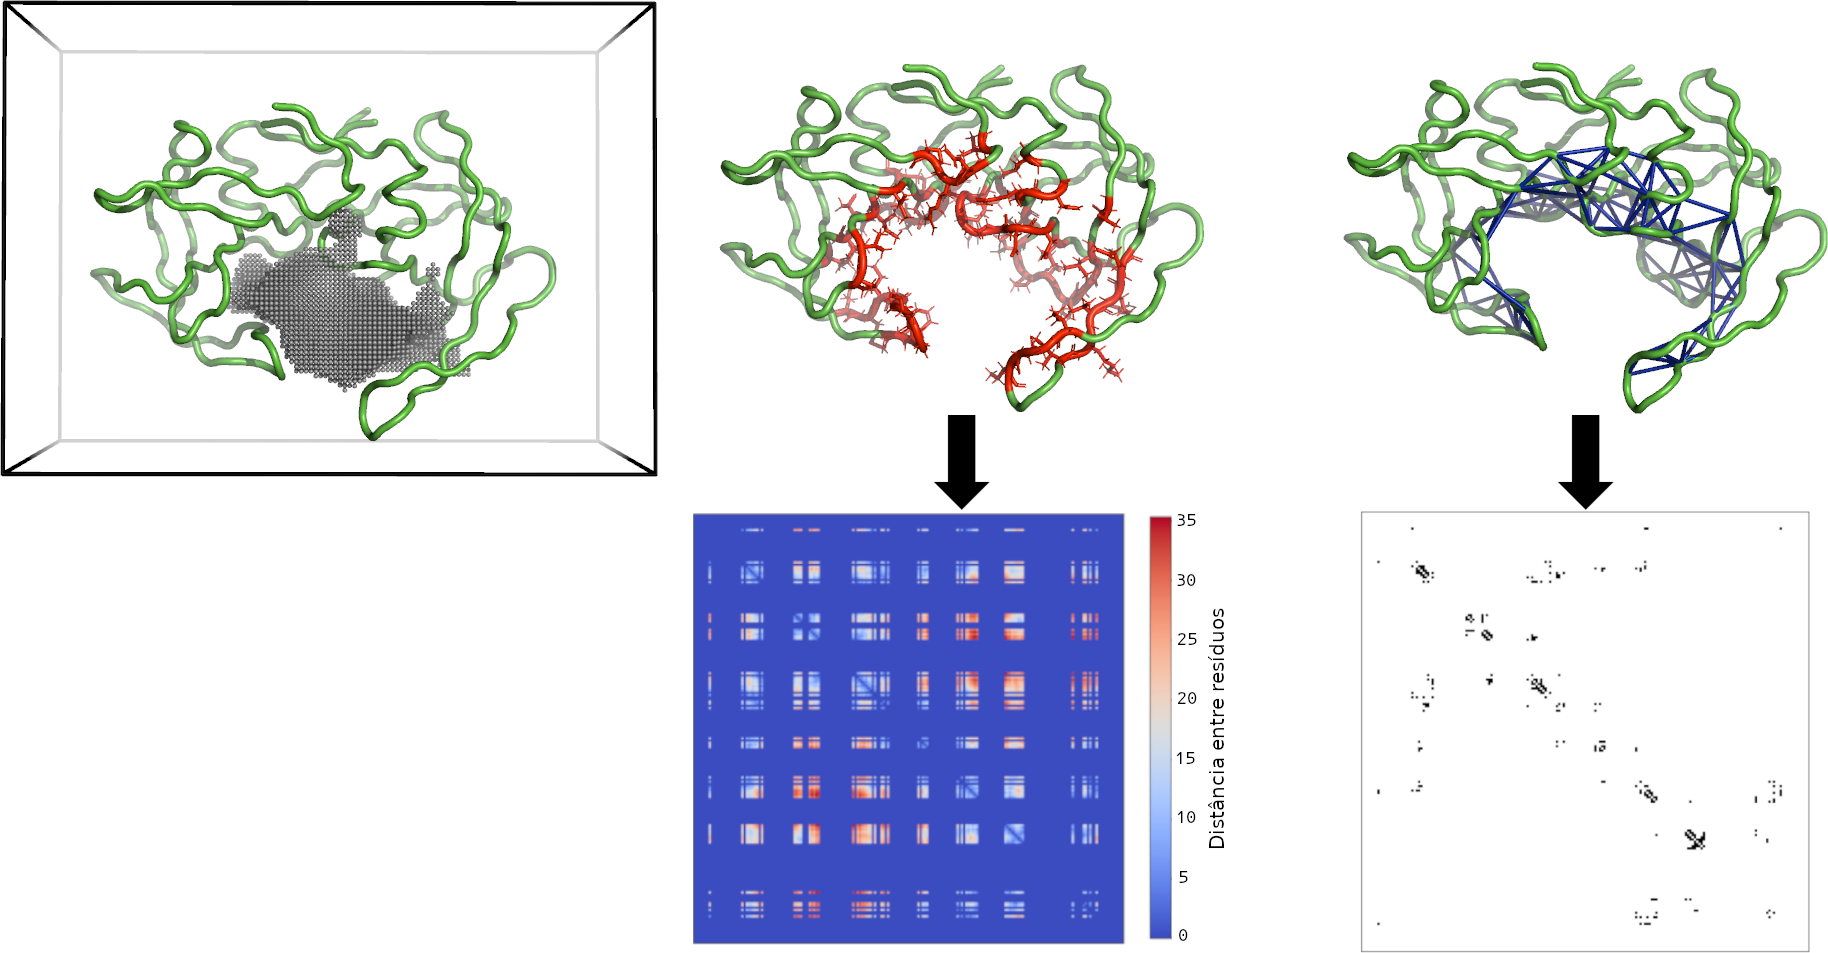
\includegraphics[scale=1]{images/HIV-1-representation.png}
  \caption[Codificação de dados para estudo de similaridade de cavidades da HIV-1 protease ao longo da trajetória de dinâmica molecular]{\textbf{Codificação de dados para estudo de similaridade de cavidades da HIV-1 protease ao longo da trajetória de dinâmica molecular.} Representação da cavidade do sítio ativo em grade 3D (quadro esquerdo), onde os pontos de cavidade são identificado por 1, enquanto os demais pontos (pontos de biomolécula, pontos de meio e pontos de espaço vazio) identificados o valor 0. Representação topológica do sítio ativo (quadro central), onde abstraímos as cavidades como um matriz de distância, ordenados pela sequência da proteína. Representação em forma de grafo das relações entre os resíduos do sítio ativo (quadro direito), onde abstraímos as cavidades como um matriz de contatos, ordenados pela sequência da proteína.}
  \label{fig:hiv-1-representation}
\end{figure}

Nesse caso de estudo, detectamos 672 cavidades ao longo dos 201 quadros de simulação, \ie, teremos 672 estruturas de dados a serem agrupadas por agrupamento hierárquico, explorando as métricas de afinidade apropriadas para cada representação. Para vetores booleanos, avaliamos as seguintes métricas disponíveis no pacote SciPy \cite{scipy}: dissimilaridade de Dice ($d_{Dice}$; Equação \ref{eq:dice}), distância de Hamming, dissimilaridade de Jaccard-Needham, dissimilaridade de Kulczynski, dissimilaridade de Rogers-Tanimoto, dissimilaridade de Russell-Rao, dissimilaridade de Sokal-Michener, dissimilaridade de Sokal-Sneath e dissimilaridade de Yule. Para vetores numéricos, avaliamos as seguintes métricas disponíveis no pacote SciPy \cite{scipy}: distância de correlação ($\rho$; Equação \ref{eq:correlacao}), distância de Bray-Curtis, distância de Canberra, distância Chebyshev, distância de Manhattan (também conhecido como distância de \textit{City Block}), distância de Cosseno ($d_{Cosseno}$; Equação \ref{eq:cosseno}), distância de Jensen-Shannon e distância quadrática Euclidiana. 

\begin{equation}
  d_{Dice}(u,v) = \frac{c_{VF} + c_{FV}}{2c_{VV} + c_{FV} + c_{VF}}, d_{Dice} \in [0, 1], 
  \label{eq:dice}
\end{equation}

onde $c_{ij}$ é o número de ocorrências de $u[k] = i$ e $v[k] = j$ para $k<n$.

\begin{equation}
  \rho(u,v) = 1 - \frac{(u - \bar{u}) \cdot (v - \bar{v})}{{\|(u - \bar{u})\|}_2 {\|(v - \bar{v})\|}_2}, \rho \in [-1, 1],
  \label{eq:correlacao}
\end{equation}

onde $\bar{u}$ é a média dos elementos de $u$, $\bar{v}$ é a média dos elementos de $v$, e $x \cdot y$ é o produtor escalar de $x$ e $y$.

\begin{equation}
  d_{Cosseno}(u,v) = 1 - \frac{u \cdot v}{\|u\|_2 \|v\|_2}, d_{Cosseno} \in [-1, 1],
  \label{eq:cosseno}
\end{equation}

onde $u \cdot v$ é o produtor escalar de $u$ e $v$.

Como não existe um verdade absoluta para o agrupamento das cavidades, utilizamos o Coeficiente de Silhueta (\textit{Silhouette Score}, em inglês; Equação \ref{eq:silhouette-score}) para maximizar a semelhança entre membros de um grupo e a diferença entre membros de grupos distintos, onde o melhor valor é 1, o pior é -1 e 0 indica agrupamentos sobrepostos. Assim, valores negativos geralmente indicam que uma amostra está no grupo errado, já que um grupo diferente é mais similar à amostra do que o grupo que ela está atribuída. Por fim, é importante destacar que os coeficientes de silhueta não podem ser comparados entre diferentes métricas de afinidade. Portanto, comparamos os métodos com base no número ideal de grupos identificados pelo coeficiente de silhueta máximo dentro de uma mesma métrica de afinidade.

\begin{equation}
  Coeficiente\;de\;Silhueta = \frac{(b - a)}{max(a, b)}, Coeficiente\;de\;Silhueta \in [-1, 1],
  \label{eq:silhouette-score}
\end{equation}

onde $a$ é a distância média intra-cluster e $b$ é a distância para o cluster mais próximo para cada amostra.

Em seguida, aplicamos o algoritmo de agrupamento hierárquico não supervisionado, otimizando o coeficiente de silhueta para cada métrica de afinidade, utilizando o método de ligação completo (Figura \ref{fig:hiv-1-clustering-results}). Para a representação em grade 3D, não exploramos diferentes métricas de afinidade devido ao tamanho dos dados ($\aproximadamente 10^6$ pontos por cavidade), e portanto, utilizamos a distância de correlação (Equação \ref{eq:correlacao}), onde encontramos 10 grupos com um coeficiente de silhueta máximo de $\aproximadamente 0{,}42$. Com a simplificação do tamanho dos dados para as duas representações restantes ($\aproximadamente 10^4$ pontos por cavidade), foi possível explorar as métricas de afinidade apropriadas. Para a representação topológica, a distância de cosseno (Equação \ref{eq:cosseno}) apresentou o maior número de grupos entre as métricas numéricas (\ie, 15 grupos) com um coeficiente de silhueta máximo de $\aproximadamente 0{,}54$. Para a representação em forma de grafo, a dissimilaridade de Dice (Equação \ref{eq:dice}) apresentou o maior número de grupos entre as métricas numéricas (\ie, 16 grupos) com um coeficiente de silhueta máximo de $\aproximadamente 0{,}52$.

\begin{figure}[h]
  \centering
  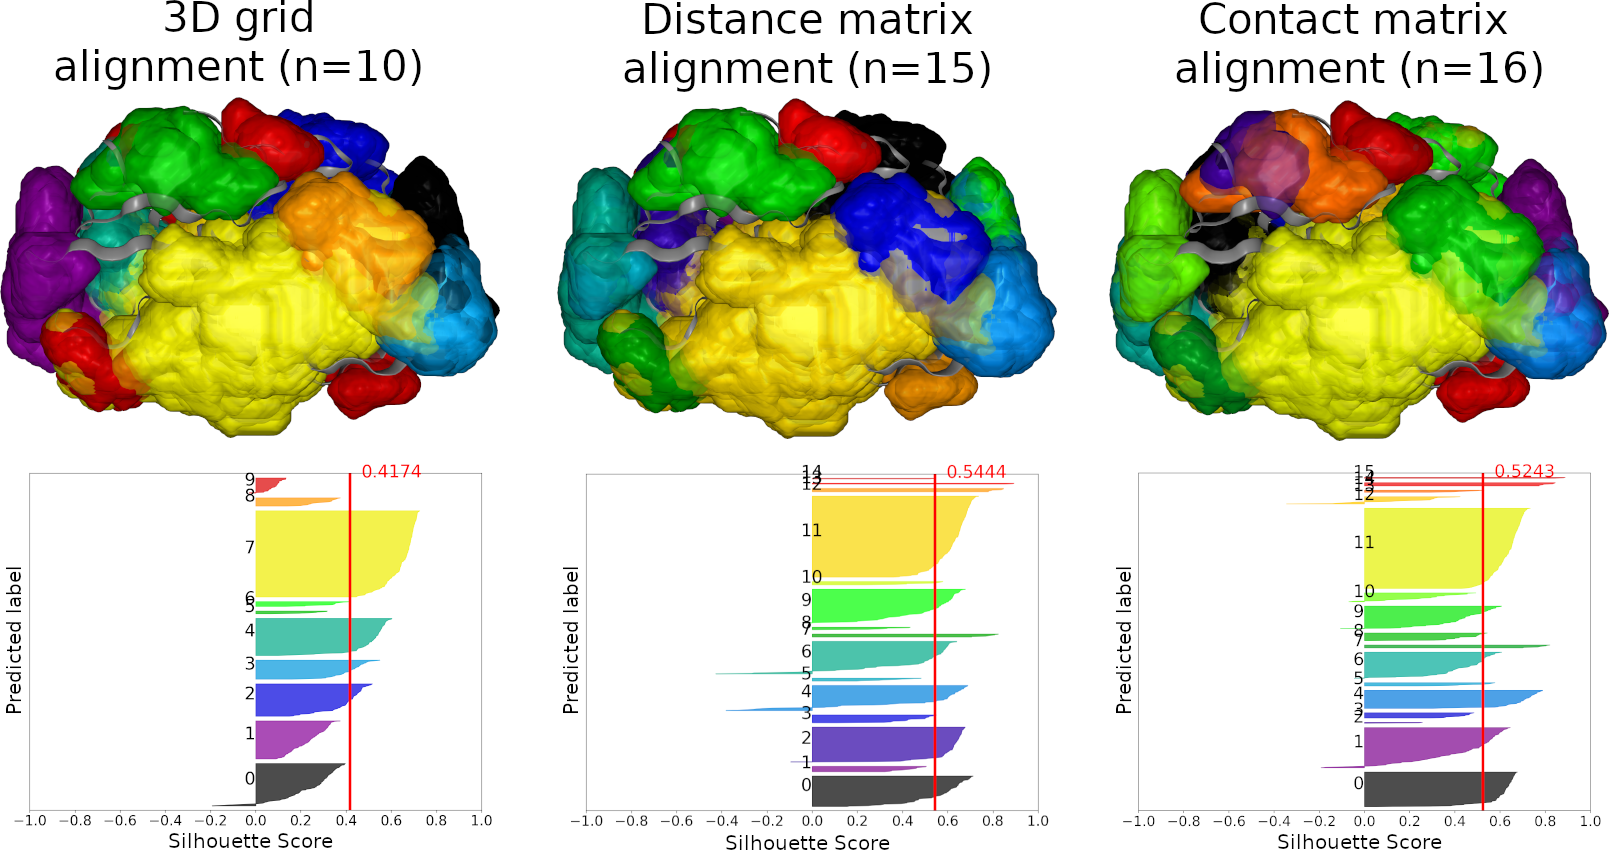
\includegraphics[scale=1.1]{images/HIV-1-clustering-results.png}
  \caption[Agrupamento hierárquico das cavidades da protease do HIV-1]{\textbf{Agrupamento hierárquico das cavidades da protease do HIV-1.} Todas as cavidades detectadas ao longo da dinâmica molecular foram sobrepostas na mesma estrutura e coloridas de acordo com os rótulos atribuídos pelo agrupamento hierárquico da grade 3D (quadro esquerdo), da matriz de distâncias (quadro central) e da matriz de contatos (quadro direito). O gráfico de coeficiente de silhueta é apresentado para cada amostra de acordo com o rótulo atribuído. A linha vermelha indica o valor do coeficiente de silhueta médio para o agrupamento hierárquico.}
  \label{fig:hiv-1-clustering-results}
\end{figure}

A partir desses agrupamentos, conseguimos agrupar com sucesso as cavidades e acompanhar a evolução delas ao longo da simulação de DM. Isso simplificou a comparação das características entre as cavidades ao longo do tempo. O uso das matrizes de distância e matrizes de contatos mostrou-se efetivo devido à sua capacidade de agrupar as cavidades. Além disso, essas representações foram mais rápidas e simples para agrupar as cavidades ao longo do tempo em simulações de DM, já que o algoritmo de agrupamento hierárquico tem uma complexidade de aproximadamente $\mathcal{O}(n^3)$ e o tamanho dos dados diminui em 100 vezes por cavidade em comparação com a estrutura original. Portanto, considerando que temos 672 cavidades nesse caso de estudo, a redução do uso de memória é de aproximadamente 67200 vezes.

\subsection{Discussão}

A aplicação do KVFinderMD ilustra a integração das ferramentas disponíveis no KVFinder suite (\ie, pyKVFinder e SERD) para realizar uma análise sistemática de cavidades por meio de um protocolo automatizado. Ao utilizar algoritmos de agrupamento hierárquico e diferentes métricas de afinidade em várias representações (grade 3D, representação topológica e representação em grafo), pudemos identificar grupos de cavidades mais similares, o que nos permitiu avaliar a evolução temporal dos sítios de ligação. Além disso, conseguimos reduzir o tamanho dos dados necessários para a análise e simplificar a comparação entre as cavidades em simulações de DM, demonstrando uma aplicabilidade prática do KVFinder suite.

A análise da similaridade das cavidades da protease do HIV-1 ao longo da simulação de DM nos permitiu acompanhar a evolução dessas cavidades e comparar suas características ao longo do tempo, como apresentado na Figura \ref{fig:hiv1-protease-dm-analysis}. Isso foi realizado sem interferência humana, utilizando os recursos automatizados do KVFinderMD. No entanto, é importante ressaltar que, embora o KVFinderMD seja uma ferramenta útil para a análise de cavidades em simulações de DM, existem algumas limitações a serem consideradas. Por exemplo, a escolha das métricas de afinidade e dos parâmetros de agrupamento hierárquico pode influenciar os resultados obtidos. Portanto, é fundamental realizar uma avaliação cuidadosa e explorar diferentes configurações para obter os melhores resultados. % Além disso, a detecção de cavidades em simulações de DM depende da precisão e qualidade das estruturas conformacionais geradas durante a simulação. Variações conformacionais insuficientes podem levar à detecção de cavidades menos representativas ou à perda de informações importantes. Portanto, é necessário considerar esses aspectos ao interpretar os resultados obtidos com o KVFinderMD.

Apesar dessas limitações, o KVFinderMD representa um avanço significativo no estudo das interações biomoleculares ao longo do tempo. Sua capacidade de automatizar a análise de cavidades em simulações de DM, combinada com as outras ferramentas do KVFinder suite, oferece uma abordagem abrangente para investigar os sítios de ligação e compreender sua evolução. Isso pode ser útil no desenvolvimento de estratégias terapêuticas e no desenho racional de novos fármacos, especialmente em sítios de ligação transientes.

% \section{\textit{Benchmarking} das ferramentas disponíveis}

%%% Chapter 5

\chapter{Conclusão}

Após estudo cuidadoso das demandas de ferramentas computacionais da comunidade de biologia estrutural, desenvolvemos com sucesso a plataforma computacional KVFinder suite. Essa plataforma foi projetada para estudos de sistemas biomoleculares, fornecendo ferramentas abrangentes de codificação e caracterização de biomoléculas e seus sítios de ligação. O KVFinder suite é composto por 5 ferramentas computacionais, englobando diferentes demandas e objetivos da comunidade de biologia estrutural, que são o KVFinder-web, parKVFinder, pyKVFinder, SERD e KVFinderMD. 

O KVFinder-web é uma aplicação web de código aberto para detecção e caracterização de cavidades, usando o parKVFinder, em qualquer tipo de estrutura biomolecular. O KVFinder-web visa ampliar o uso do parKVFinder na comunidade científica, além de democratizar o acesso e remover barreiras para usuários que não possuem conhecimento técnico para instalar e configurar uma ferramenta computacional, que possuem recursos computacionais limitados ou que desejam realizar uma análise simples e rápida. A aplicação web está disponível em \url{https://kvfinder-web.cnpem.br}.

O parKVFinder é uma ferramenta de código aberto desenvolvida para a detecção e caracterização de cavidades biomoleculares. Ele inclui um plugin gráfico integrado ao visualizador molecular PyMOL, que oferece uma interface intuitiva para explorar parâmetros personalizáveis e visualizar as cavidades detectadas e suas características. Embora o parKVFinder tenha limitações em aplicações automatizadas e comparações sistemáticas de sítios de ligação, ele desempenha um papel importante na otimização dos parâmetros de detecção e caracterização por meio do plugin gráfico do PyMOL (PyMOL2 parKVFinder Tools), devido aos seus recursos visuais. Estes parâmetros otimizados podem ser posteriormente adotados em estudos automatizados e comparações sistemáticas de sítios de ligação.

O pyKVFinder é um pacote Python de código aberto para detectar e caracterizar cavidades em estruturas biomoleculares em protocolos automatizados e aplicações de ciência de dados. Além de possuir as mesmas funcionalidades do KVFinder-web e parKVFinder, o pyKVFinder fornece estruturas de dados acessíveis e flexíveis no ecossistema Python, como \textit{ndarrays} e dicionários. Isso permite que os usuários desenvolvam novas caracterizações de cavidades e protocolos de análise baseados nessas estruturas de dados, facilitando a exploração eficiente e eficaz das cavidades biomoleculares e impulsionando a descoberta de novos alvos terapêuticos e o desenvolvimento de medicamentos mais eficazes.

Dentro do contexto do pyKVFinder, em colaboração com o Dr. György Szalóki, expandimos a metodologia de detecção e caracterização de cavidades para uma nova classe de moléculas chamadas de gaiolas supramoleculares. Além disso, desenvolvemos novas caracterizações aplicáveis tanto à gaiolas quanto à biomoléculas, incluindo a modelagem da superfície molecular em grades 3D, a estimativa de volume molecular e a caracterização de aberturas das cavidades. Essas implementações podem servir como guia para os usuários desenvolverem novas caracterizações.

Ao longo do projeto, avaliamos continuamente o desempenho computacional e a capacidade de detecção de cavidades das ferramentas do KVFinder suite (\eg, KVFinder-web, parKVFinder e pyKVFinder), comparando-as com outras metodologias disponíveis. Os resultados atestaram a eficácia e o desempenho computacional dessas ferramentas. No entanto, estas ferramentas citadas acima dependem da modelagem e descrição em grades 3D. Para abranger uma gama mais ampla de codificações de biomoléculas e sítios de ligação, desenvolvemos a ferramenta SERD. Essa ferramenta expandiu as possibilidades de codificação na plataforma KVFinder suite, incluindo a representação topológica dos resíduos de interface e a representação em forma de grafos. Essa flexibilidade permite a aplicação de diferentes codificações em estudos de sistemas biomoleculares.

Por fim, desenvolvemos o KVFinderMD, um pacote em Python que permite explorar a dinâmica dos sítios de ligação em estruturas biomoleculares de interesse farmacológico. Essa ferramenta exemplifica a capacidade do pyKVFinder de fornecer protocolos automatizados para análises sistemáticas de sítios de ligação. A análise da similaridade das cavidades da protease do HIV-1 ao longo de uma simulação de DM permitiu acompanhar a evolução das cavidades e comparar suas características ao longo do tempo. Utilizando algoritmos de agrupamento hierárquico e diferentes métricas de afinidade em diferentes codificações (\ie, representações em grade 3D, representação topológica e representação em grafo), identificamos grupos de cavidades mais similares. Além disso, pudemos reduzir o tamanho dos dados necessários à análise de similaridade e simplificar da comparação entre as cavidades em simulações de DM, demonstrando a aplicabilidade prática do KVFinder suite.

Em resumo, a plataforma computacional KVFinder suite simplifica o estudo de sistemas biomoleculares de interesse terapêutico, incluindo a caracterização de biomoléculas e seus sítios de ligação, mesmo para usuários menos experientes. Isso tem um impacto direto na busca e no desenho racional de fármacos, assim como na compreensão das estruturas de biomoléculas.

% As referências:
\bibliographystyle{abnt-num}
\bibliography{phdquali}

% Os anexos, se houver, vêm depois das referências:
\appendix

\chapter{Casos de estudo aplicando as ferramentas do KVFinder suite \label{ap:casos-de-estudo}}

Nesta seção, apresentamos os casos de estudo aplicando as ferramentas do KVFinder suite: parKVFinder, pyKVFinder e KVFinder-web.

\section{parKVFinder \label{ap:casos-de-estudo-parkvfinder}}

\subsection{Dinâmica molecular da HIV-1 protease \label{sec:md-hiv1-protease}}

O sítio ativo da HIV-1 protease é um alvo terapêutico relevante, que é alvo de diversos medicamentos antiretrovirais. Este sítio de ligação possui uma grade complexidade estrutural e morfológica devido à movimentação dos \textbeta-hairpins, conhecidos como \textit{flaps}. Seu volume varia de acordo com a movimentação dos \textit{flaps}, que controlam a acessibilidade do substrato ao sítio ativo do homodímero \cite{lam1994,soares2016}. 

Nesse estudo, foi investigado a DM da HIV-1 protease por meio da identificação e avaliação do volume do sítio ativo durante simulações de DM. O objetivo era descrever a dinâmica de movimentação dos \textit{flaps} através do volume e forma da cavidade do sítio ativo como descritores conformacionais durante as simulações de MD. Para isso, foram realizadas simulações de DM por 200 ns, usando o pacote GROMACS 2019.4 \cite{gromacs}, o campo de força AMBER99SB-ws e o modelo de água TIP42005s, partindo da estrutura cristalográfica da protease do HIV-1 na conformação fechada \cite{lam1994}, sem o inibidor presente na estrutura, a ureia cíclica.

O volume do sítio ativo foi acompanhado ao longo das simulações (Figura \ref{fig:hiv1-protease-dm-analysis}). Observou-se que o volume inicial da cavidade corresponde à conformação fechada (linha verde) e, após cerca de 25 ns, aumenta até atingir o valor correspondente à conformação semi-aberta (linha vermelha) em cerca de 75 ns, indicando um processo de abertura ao longo da simulação. Posteriormente, os \textit{flaps} se afastam ainda mais, e a cavidade atinge seu volume máximo em cerca de 175 ns, antes de reverter para a conformação semi-aberta, que é mais estável. Essa dinâmica de mudança de volume correlaciona-se (correlação de Pearson; $\rho = 0,72$) com o desvio médio quadrático (RMSD; \textit{Root-mean-square deviation}, em inglês) do C\textalpha\space calculado a partir da conformação fechada como referência, indicando uma descrição adequada do estado conformacional da proteína ao longo da simulação. É importante destacar que o RMSD é uma métrica que descreve variações globais na estrutura, enquanto o volume estimado é uma métrica direta das mudanças conformacionais do sítio ativo, possivelmente relacionadas à acessibilidade do ligante.

\begin{figure}[h]
  \centerline{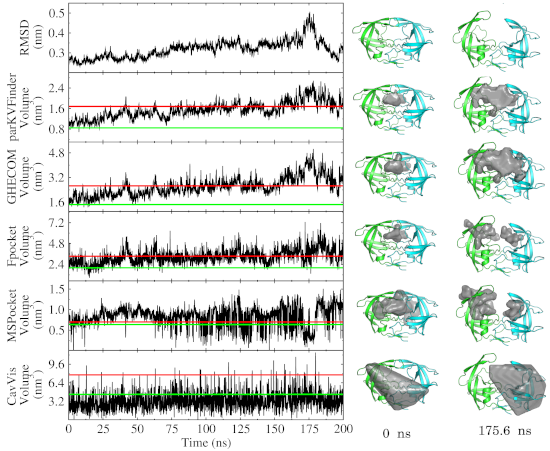
\includegraphics[scale=0.8]{images/hiv1-protease-md-analysis.png}}
  \caption[Volume de seu sítio ativo HIV-1 protease ao longo de uma simulação de dinâmica molecular de 200 ns]{\textbf{Volume de seu sítio ativo HIV-1 protease ao longo de uma simulação de dinâmica molecular de 200 ns.} As linhas verdes e vermelhas indicam o volume da cavidade para os estados fechado (PDB ID: 1HVR) e semi-aberto (PDB ID: 1HHP), respectivamente. As estruturas da proteína no início da simulação (0 ns) e no quadro com o maior RMSD (175.6 ns) são mostradas como diagramas. As cavidades correspondentes detectadas por cada ferramenta são mostradas como superfícies cinzas.}
  \label{fig:hiv1-protease-dm-analysis}
\end{figure}

Comparou-se o desempenho do parKVFinder \cite{guerra2020} com outros programas baseados em geometria (Figura \ref{fig:hiv1-protease-dm-analysis}), \ie, GHECOM \cite{ghecom}, Fpocket \cite{fpocket}, MSPocket \cite{mspocket} e CavVis \cite{cavvis}. Primeiramente, avaliou-se a correlação do volume estimado por cada programa e o RMSD, assim como realizado para o parKVFinder. O volume estimado pelo GHECOM ($\rho = 0,75$) também se correlaciona ao estado conformacional, semelhante ao parKVFinder ($\rho = 0,72$), possivelmente porque ambos empregam métodos baseados em grade e esfera. No entanto, as cavidades encontradas pelos programas Fpocket ($\rho = 0,35$), MSPocket ($\rho = -0,24$) e CavVis ($\rho = 0,19$) não apresentaram uma correlação satisfatória com a dinâmica conformacional do sítio ativo. Portanto, parKVFinder e GHECOM apresentaram uma alta acurácia na descrição do estado conformacional do sítio ativo da HIV-1 protease. 

Além de boa acurácia, também foi avaliado o tempo computacional dos programas. O parKVFinder ($t = 1h03m$) foi pelo menos quatro vezes mais rápido que o GHECOM ($t = 4h32m$), devido às subrotinas de múltiplas \textit{threads} implementadas no parKVFinder. Além disso, o parKVFinder também superou o MSPocket ($t = 2h48m$) e o CavVis ($t = 3h45$) em termos de tempo computacional, mas não superou o Fpocket ($t = 20m$), que utiliza um método baseado em tesselação de Voronoi e esferas alfa, sendo rapidamente computado. No entanto, essa implementação do Fpocket mostrou-se menos sensível na descrição detalhada do sítio ativo da HIV-1 protease, não diferenciando eficientemente os estados conformacionais do sítio ativo. Portanto, considerando a acurácia e o desempenho, o parKVFinder destacou-se como uma opção robusta para a detecção e caracterização espacial de cavidades no caso de estudo da HIV-1 protease \cite{guerra2020}.

É importante ressaltar que os resultados completos e detalhes das simulações e análises estão disponíveis no artigo publicado no periódico \textit{SoftwareX} \cite{guerra2020}.

\subsection{Mayaro e outros alphavírus}

O vírus Mayaro (MAYV) é um arbovírus emergente das Américas Central e do Sul que pode causar uma doença debilitante e artritogênica. As proteínas E1 e E2 são importantes proteínas virais transmembranares organizadas em heterodímeros. Trímeros de heterodímeros de E1 e E2 compõem as espículas na superfície viral, que se estendem através da bicamada lipídica e interagem com as proteínas nucleocapsídicas C. As espículas estão envolvidas na ligação aos receptores celulares, internalização nas células e fusão de membrana. A liberação do RNA do MAYV no citoplasma resulta na expressão de proteínas virais, replicação viral e culmina na geração de progênie viral madura e infecciosa. As proteínas E1 e E2 do MAYV são os principais alvos para o desenvolvimento de vacinas e medicamentos antivirais \cite{ribeiro2021}. No entanto, a falta de informações estruturais sobre as proteínas E1 e E2 do MAYV tem dificultado o desenvolvimento de novas estratégias para combater a infecção pelo MAYV.

A região central entre as proteínas E1 e E2 forma uma cavidade que é ocupada por uma densidade extra longa, que não pode ser explicada por resíduos de cadeia lateral (Figura \ref{fig:mayv-e1-e2}A e B). Um perfil de densidade similar foi observado anteriormente em um mapa crioeletrônico do vírus Sindbis (SINV), e os autores propuseram que uma cauda fosfolipídica hidrofóbica (C18), chamada de \textit{pocket factor} (fator de bolsão, em português), poderia ocupar essa densidade e estabilizar o bolsão hidrofóbico formada entre E1 e E2 \cite{chen2018}.

\begin{figure}[hp]
  \centerline{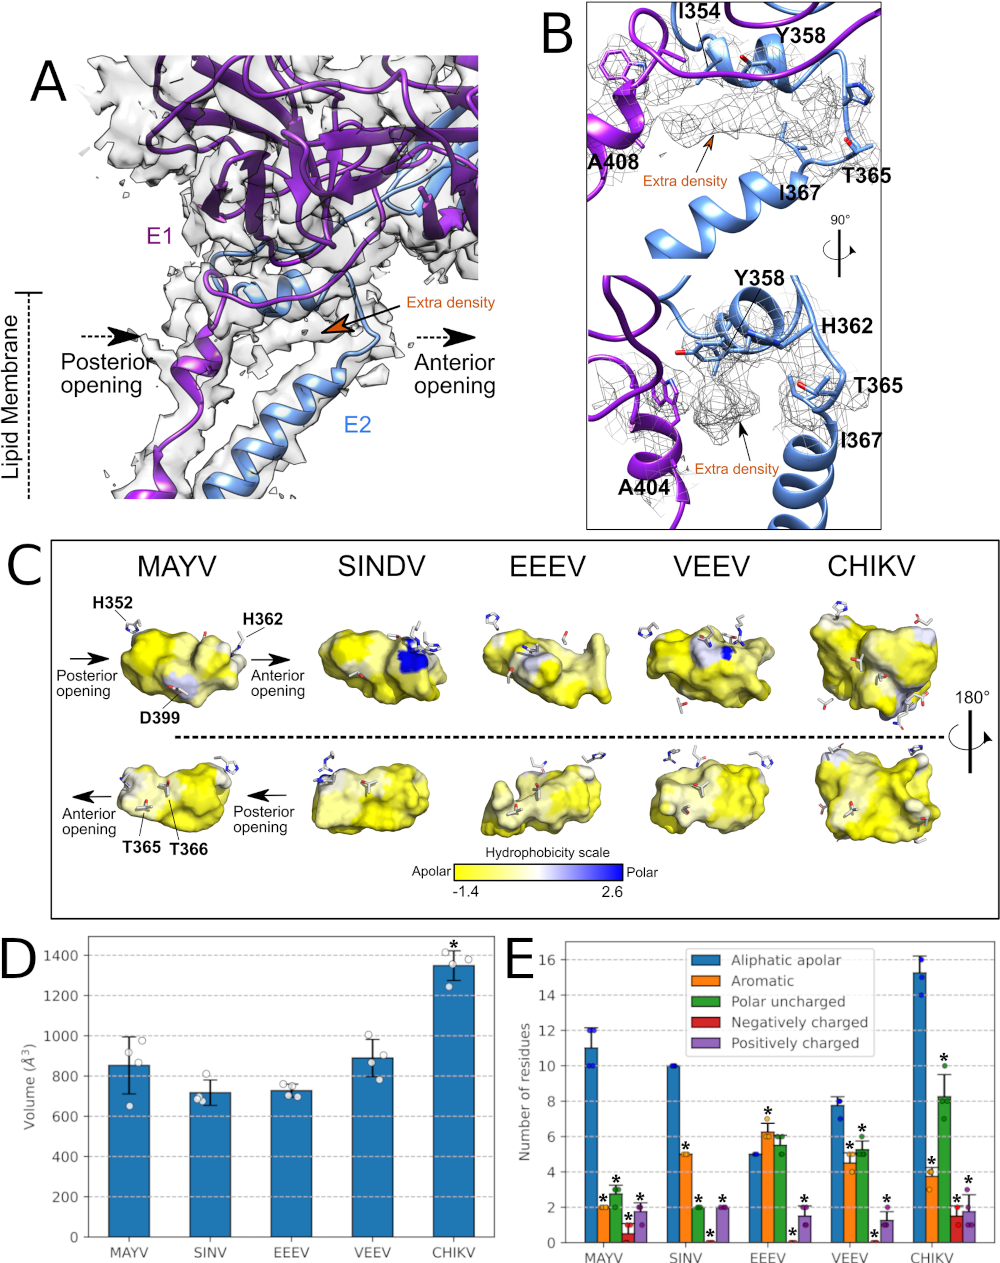
\includegraphics[scale=1]{images/mayv-e1-e2.png}}
  \centerline{\scriptsize{\textbf{Fonte:} Adaptado de \cite{ribeiro2021}.}}
  \caption[Domínios transmembranares E1 e E2 do MAYV e a cavidade hidrofóbica]{\textbf{Domínios transmembranares E1 e E2 do MAYV e a cavidade hidrofóbica.} \textbf{(A)} Modelo atômico 3D do MAYV ajustado ao mapa de densidade, mostrando a porção superior das hélices TM de E1 e E2. A interseção entre E1-E2 forma uma cavidade com abertura anterior e posterior. A densidade extra observada dentro da cavidade está indicada. \textbf{(B)} Detalhe da densidade extra encontrada na região da cabeça de E1-E2 e os resíduos ao redor. O mapa de densidade do MAYV está representado em superfície ou malha. \textbf{(C)} Prospeção da cavidade em estruturas de alphavírus. A cavidade entre os domínios E1 e E2 está representada em superfície e colorida com base na escala de consenso de Eisenberg, utilizando os resíduos que formam a cavidade, conforme detalhado na seção de métodos. Apenas os resíduos polares estão representados como sticks. \textbf{(D)} Volume da cavidade estimado para os quatro heterodímeros E1-E2 (n = 4 estruturas independentes de heterodímeros) na unidade assimétrica. Um teste ANOVA unidirecional com comparação múltipla de Tukey foi utilizado para comparar o volume da cavidade do MAYV com outros alphavírus (* indica adj. p < 0,01 quando comparado aos alphavírus com MAYV). \textbf{(E)} Número de resíduos em cada um dos quatro heterodímeros E1-E2 (n = 4 estruturas independentes de heterodímeros) na unidade assimétrica, separados por classes. Um teste ANOVA unidirecional com comparação múltipla de Tukey foi utilizado para comparar o número de resíduos na classe alifática apolar com as outras classes na mesma espécie de alphavírus (* indica adj. p < 0,01 quando comparando a classe alifática apolar com as outras classes). Todos os dados são apresentados como valores médios +/- DP. Alifática apolar: ALA, VAL, ILE, LEU, GLY, PRO; Aromática: PHE, TYR, TRP; Polar não carregada: SER, THR, CYS, MET, ASN, GLN; Carregada negativamente: GLU, ASP; Carregada positivamente: ARG, LYS, HIS.}
  \label{fig:mayv-e1-e2}
\end{figure}

Para compreender melhor o ambiente do bolsão e extrair suas características químicas, o bolsão completo do MAYV foi caracterizada usando o parKVFinder \cite{guerra2020} e comparado com os bolsões de outros alphavírus. Os ectodomínios de E1 e E2 do MAYV (PDB ID: 7KO8), SINDV (PDB ID: 6IMM), vírus da Encefalite Equina Oriental (EEEV; PDB ID: 6MX4), vírus da Encefalite Equina Venezuelana (VEEV; PDB ID: 3J0C) e Vírus Chikungunya (CHIKV; PDB ID: 6NK5) foram usados para detecção e caracterização do bolsão hidrofóbico. No MAYV, a cavidade entre os domínios E1 e E2 possui um volume de $\aproximadamente850 \mAA^3$ (Figura \ref{fig:mayv-e1-e2}D). Esse volume é bastante semelhante em SIND, EEEV e VEEV, mas em CHIKV, E1 e E2 estão mais distantes um do outro, o que cria um volume maior.

A natureza hidrofóbica do bolsão em alphavírus é claramente observada pelo mapeamento da superfície de hidrofobicidade (Figura \ref{fig:mayv-e1-e2}C) e pelo número de resíduos apolares que formam o núcleo da cavidade (Figura \ref{fig:mayv-e1-e2}E). A densidade do bolsão se estende até resíduos polares, como H362, T365 e T366 do domínio E2 na abertura posterior (Figura \ref{fig:mayv-e1-e2}C e E), indicando que a molécula pode ter uma natureza anfipática, como um ácido graxo. T365 e T366 têm uma posição estrutural conservada em outros alphavírus ou são substituídos por serina, um resíduo ainda mais polar. Na abertura posterior, outra histidina (H352 do E2) ajuda a fechar o bolsão. A maioria dos alphavírus, exceto o SINV, possui resíduos de histidina ocupando uma posição semelhante. Em conjunto, essas descobertas indicam que os alphavírus têm uma cavidade anfipática consistente formada entre os domínios E1 e E2 na membrana externa da bicamada lipídica. Caso o bolsão alphaviral seja ocupado por uma molécula, essa molécula seria quimicamente similar em diferentes alphavírus. O mapa de densidade do MAYV sugere que a densidade extra pode ser ocupada por um ácido graxo que pode aprimorar as interações entre E1 e E2. Portanto, o bolsão pode ser alvo para o desenvolvimento de compostos antivirais contra o MAYV e outros alphavírus, usando o desenho racional de fármacos.

Por outro lado, as proteínas nucleocapsídicas C dos alphavírus são compostas por dois subdomínios: um domínio N-terminal desordenado que se liga ao RNA viral, que não é observado no mapa de densidade do MAYV, e um domínio C-terminal estruturado que se liga às proteínas E2 (Figura \ref{fig:mayv-c-e2}). A região N-terminal tem menor identidade entre os alphavírus e é relatada como específica do vírus \cite{ribeiro2021}.

\begin{figure}[hp]
  \centerline{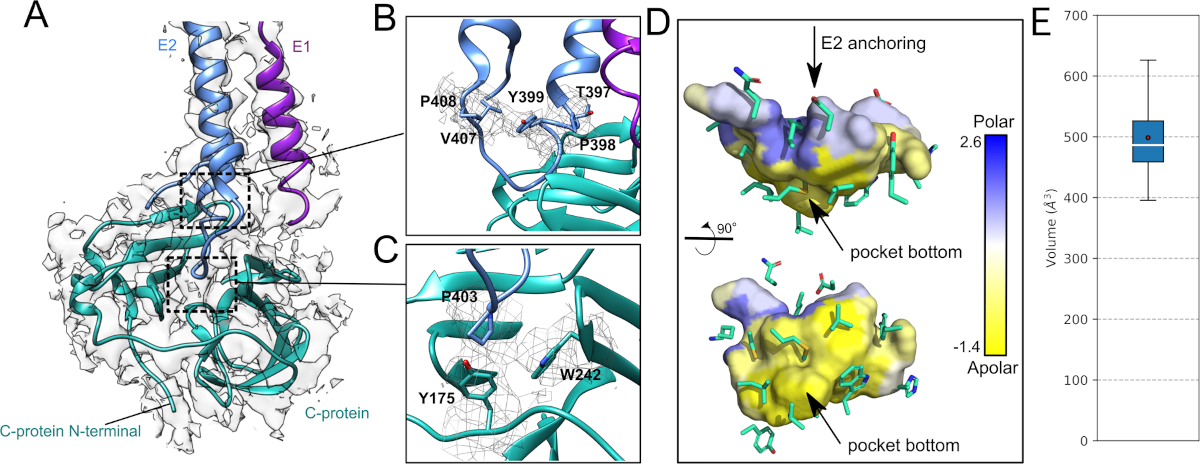
\includegraphics[scale=1]{images/mayv-c-e2.png}}
  \centerline{\scriptsize{\textbf{Fonte:} Adaptado de \cite{ribeiro2021}.}}
  \caption[Interação da cápside do MAYV com o domínio C-terminal da proteína E2]{\textbf{Interação da cápside do MAYV com o domínio C-terminal da proteína E2.} \textbf{(A)} Modelo atômico 3D do MAYV ajustado ao mapa de densidade obtido por criomicroscopia eletrônica. As proteínas C, E1 e E2 são representadas como desenhos em ciano, roxo e azul, respectivamente. \textbf{(B)} A interação do motivo TPY (resíduos T387, P398 e Y399) com a proteína C. \textbf{(C)} Os resíduos P403 e T402 da E2 e sua interação com os resíduos aromáticos Y175 e W242 na proteína C. O mapa de densidade do MAYV é mostrado em representação de malha. \textbf{(D)} Prospeção da cavidade na proteína C do MAYV, mostrando um ambiente hidrofóbico na parte inferior do bolso e um ambiente polar e carregado nas bordas externas da cavidade. A cavidade da proteína C que se liga ao domínio C-terminal da E2 é representada em superfície e colorida de acordo com a escala hidrofóbica de consenso de Eisenberg. Os resíduos da proteína C que cercam a cavidade são representados como \textit{sticks}. \textbf{(E)} Boxplot do volume da cavidade estimado para as quatro cápsides (n = 4 estruturas independentes de cápside) na unidade assimétrica. No boxplot, a caixa representa a amplitude interquartil (IQR) ($67,5 \mAA^3$), o 75º percentil (Q3) ($526,2 \mAA^3$) e o 25º percentil (Q1) ($458,7 \mAA^3$). A linha central indica a mediana ($486,3 \mAA^3$) e a média ($498,6 \mAA^3$) é indicada por um ponto. As "whiskers" com valor mínimo ($395,7 \mAA^3$) e valor máximo ($626,2 \mAA^3$) são determinadas usando Q1-1,5 x IQR e Q3+1,5 x IQR, respectivamente.}
  \label{fig:mayv-c-e2}
\end{figure}

O mapa de densidade do MAYV confirma a estrutura geralmente conservada da proteína C, formando dois subdomínios ricos em folhas beta separados por uma cavidade rasa ($\aproximadamente500 \mAA^3$, Figura \ref{fig:mayv-c-e2}), na qual o domínio C-terminal da proteína E2 se liga não covalentemente. O fundo do bolsão é hidrofóbico, enquanto seu topo possui resíduos polares e carregados. A interface entre o capsídeo e a proteína E2 envolve o motivo de consenso TPY (resíduos T387, P398 e Y399; Figura \ref{fig:mayv-c-e2}), que é conservado dentro do gênero \textit{Alphavirus}. Curiosamente, pequenas moléculas propostas para inibir a interação entre o capsídeo e a proteína E2 contêm anéis heterocíclicos, o que reforça a relevância desse tipo de contato para a interação entre o capsídeo e a proteína E2 e destaca esse sítio como um potencial alvo de drogas.

É importante ressaltar que os resultados completos e detalhes das análises estão disponíveis no artigo publicado no periódico \textit{Nature Communications} \cite{ribeiro2021}.

\section{pyKVFinder \label{ap:casos-de-estudo-pykvfinder}}

\subsection{SARS-CoV-2 e proteínas homólogas}

Dentre as 15 proteínas não estruturais (Nsps; \textit{Non-structural proteins}, em inglês), do novo coronavírus da Síndrome Respiratória Aguda Grave 2 (SARS-CoV-2; \textit{Severe acute respiratory syndrome coronavirus 2}, em inglês), destaca-se o domínio da fosfatase de ADP-ribose (ADRP; também conhecido como macromodomínio, MacroD) \cite{michalska2020}. Esse domínio tem sido objeto de investigação para compreender suas funções exatas no ciclo de vida do coronavírus, uma vez que o domínio ADRP reconhece ADP-ribose 1'-fosfato e parece desempenhar um papel importante na virulência e na regulação da imunidade inata à infecção \cite{fehr2016,claverie2020}. Nesse sentido, esforços recentes têm sido feitos para caracterizar o sítio de ligação de substrato de ADP-ribose e avaliar esse local como um possível alvo de drogas antivirais.

Neste contexto, utilizamos o pyKVFinder para detectar e caracterizar uma cavidade presente na proteína ADRP do SARS-CoV-2, correspondente ao sítio de ligação do substrato (Figura \ref{fig:conservation-analysis}A). Após a detecção da cavidade, caracterizamos seu volume, área e os resíduos de interface envolvidos na cavidade (Figura \ref{fig:conservation-analysis}A, quadro esquerdo). É importante ressaltar que a visualização 3D da proteína e da cavidade pode ser realizada no próprio \textit{Jupyter notebook} usando o pacote NGLView \cite{nglview}. No entanto, os usuários têm a liberdade de escolher outras ferramentas de visualização molecular (\eg, PyMOL \cite{pymol}, ChimeraX \cite{chimerax}, NGL Viewer \cite{nglviewer} ou VMD \cite{vmd}). Além disso, também inspecionamos a cavidade de ligação do substrato da ADRP em relação à profundidade (Figura \ref{fig:conservation-analysis}A, quadro central) e à hidrofobicidade (Figura \ref{fig:conservation-analysis}A, quadro direito). Essas descrições são relevantes para o desenvolvimento de medicamentos \cite{brosey2021}. Essas descrições são relevantes para o desenvolvimento de medicamentos \cite{brosey2021}. Apesar de ser exposta ao solvente na forma apo, a cavidade possui componentes internos (em vermelho) que alcançam uma porção mais central da folha-\textbeta\space da ADRP (Figura \ref{fig:conservation-analysis}A, quadro central). A análise de hidropatia mostra que o núcleo da cavidade é mais hidrofóbico (em amarelo), com alguns resíduos polares nas bordas (em azul), o que pode contribuir para o desenho racional de ligantes mais específicos.

Conforme ilustrado na Figura \ref{fig:conservation-analysis}A, o sítio de ligação do ADP-ribose forma uma fenda entre as \textalpha-hélices do domínio ADRP, e os principais contatos envolvem resíduos provenientes de regiões de alça, o que pode explicar a plasticidade do bolsão durante a ligação do substrato \cite{michalska2020}. Em seguida, determinamos a composição dos resíduos que formam a cavidade e apresentamos suas frequências em um histograma (Figura \ref{fig:conservation-analysis}B), utilizando a biblioteca matplotlib \cite{matplotlib}. No entanto, os usuários têm liberdade para analisar os dados e apresentar os resultados usando sua biblioteca gráfica preferida.

\begin{figure}[hp]
  \centering
  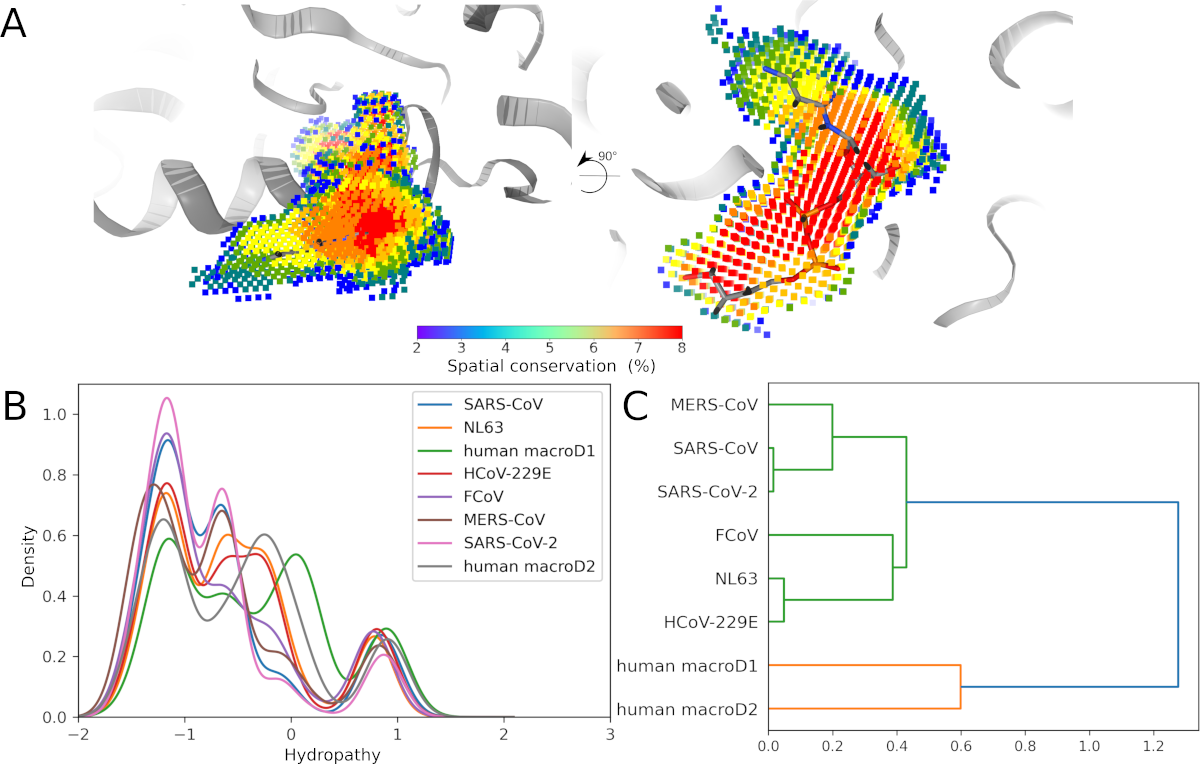
\includegraphics[scale=1]{images/adrp-sars-cov-2-conservation-analysis.png}
  \centerline{\scriptsize{\textbf{Fonte:} Adaptado de \cite{guerra2021}.}}
  \caption[Estudo do sítio de ligação do substrato da ADRP do SARS-CoV-2 e proteínas relacionadas]{\textbf{Estudo do sítio de ligação do substrato da ADRP do SARS-CoV-2 e proteínas relacionadas.} \textbf{(A)} Caracterizações do sítio de ligação do substrato do domínio ADRP do SARS-CoV-2 (PDB ID: 6WEN). Esquerda: Cavidade detectada representada como uma superfície cinza e os resíduos ao redor dela como \textit{sticks} vermelhos. Centro: Cavidade colorida por profundidade. Direita: Cavidade colorida por hidropatia usando a escala de Eisenberg e Weiss. \textbf{(B)} Gráfico de barras das frequências de resíduos de interface. Esquerda: Aminoácidos. Direita: Classes de aminoácidos. \textbf{(C)} Análise de conservação do sítio de ligação do ADP-ribose no domínio ADRP do SARS-CoV-2 (PDB ID: 6WEN, cadeia A), SARS-CoV (PDB ID: 2ACF, cadeia B), MERS-CoV (PDB ID: 5HIH, cadeia A), NL63 (PDB ID: 2VRI, cadeia A), HCoV-229E (PDB ID: 3EJG, cadeia A), FCoV (PDB ID: 3ETI, cadeia B) e proteínas macrodomínio macroD1 (PDB ID: 2X47, cadeia A) e macroD2 (PDB ID: 6Y73, cadeia D) humanas. Os pontos de cavidade que foram detectados em pelo menos duas estruturas e os pontos são coloridos por porcentagem de conservação. \textbf{(D)} Perfil de hidropatia. \textbf{(E)} Dendrograma de agrupamento hierárquico da frequência de resíduos. A métrica de correlação de Pearson foi usada para avaliar a similaridade e o método completo foi escolhido como método de ligação. Todos os gráficos e imagens foram gerados em um Jupyter notebook. As imagens das estruturas tridimensionais foram geradas utilizando o pacote NGLView \cite{nglview} enquanto os gráficos foram construídos utilizando o pacote matplotlib \cite{matplotlib}.}
  \label{fig:conservation-analysis}
\end{figure}

Para comparar a composição dessa cavidade com a de outras proteínas relacionadas, realizamos a mesma análise em sete outras proteínas selecionadas com base em homologia estrutural e alinhamento utilizando o Dali \cite{dali}. As estruturas na forma apo foram realinhadas usando o algoritmo MUSTANG \cite{mustang} do programa YASARA \cite{yasara}. Ao aplicarmos operações aritméticas nas matrizes das cavidades detectadas, determinamos a conservação da cavidade entre as espécies. Conforme observado na Figura \ref{fig:conservation-analysis}C, o núcleo da cavidade da ADRP (pontos vermelhos) é altamente conservado nas espécies analisadas, estando ocupado pelo difosfato e ribose do ADP, bem como pela segunda ribose ligada ao ADP na forma ligada ao substrato da ADRP. Por outro lado, a adenosina ocupa uma região da cavidade menos conservada (pontos azuis), o que pode indicar que a estrutura desse sítio sofre alterações em algumas espécies para acomodar o substrato ADP-ribose.

Para comparar a hidrofobicidade da cavidade entre as espécies, plotamos uma distribuição da hidrofobicidade usando a biblioteca matplotlib \cite{matplotlib}, conforme mostrado na Figura \ref{fig:conservation-analysis}D. A distribuição revela claramente a natureza hidrofóbica do bolsão, que é amplamente compartilhada entre as cavidades de ligação a substrato da ADRP dos coronavírus. Interessantemente, as proteínas humanas macroD1 e macroD2 parecem apresentar uma distribuição de hidrofobicidade menos pronunciada.

Com o pyKVFinder, é possível calcular facilmente a frequência dos resíduos que compõem a cavidade. Utilizando a biblioteca SciPy\cite{scipy}, realizamos um agrupamento (\textit{clustering}, em inglês) hierárquico dessas frequências e apresentamos o dendrograma na Figura \ref{fig:conservation-analysis}E. Nesse dendrograma, observamos que a cavidade da ADRP do SARS-CoV-2 agrupa-se com a do SARS-CoV, o que demonstra alta similaridade entre esses betacoronavírus. Próximo a eles, podemos observar outro betacoronavírus, o MERS-CoV. Por sua vez, os alphacoronavírus NL63 e HCoV-229E e o feline FCoV agrupam-se juntos. Mais distantes dos domínios dos coronavírus, encontram-se as duas proteínas humanas macrodomínio, macroD1 e D2. Apesar da cavidade da ADRP ou macroD1/D2 compartilharem o mesmo substrato, o ADP-ribose, esses resultados indicam que o perfil dos resíduos ao redor dessas cavidades segue traços evolutivos.

Para demonstrar as funcionalidades e vantagens do pyKVFinder, realizamos esse estudo em um \textit{Jupyter notebook}, onde executamos passo a passo as funções do pyKVFinder. O notebook com o caso de estudo completo está disponível em \url{https://github.com/LBC-LNBio/pyKVFinder/blob/master/examples/conservation-analysis/conservation-analysis.ipynb}. Uma descrição detalhada dessa análise está disponível no artigo publicado no periódico \textit{BMC Bioinformatics} \cite{guerra2021}. 

\subsection{Dinâmica molecular do domínio ADRP do SARS-CoV-2}

Nesse contexto, o desempenho computacional do pyKVFinder foi avaliado em simulações de DM do domínio ADRP do SARS-CoV-2 (PDB ID: 6W02, cadeia B) sem seu ligante, a ADP-ribose, por um período de 600 ns, com extração de quadros a cada 1 ns. Essa análise foi repetida com outras ferramentas bem conhecidas: parKVFinder \cite{guerra2020}, POVME \cite{povme}, fpocket \cite{fpocket}, GHECOM \cite{ghecom}, MSPocket \cite{mspocket} e Biobb\_vs \cite{biobbvs}. Todos esses métodos detectaram com sucesso o sítio de ligação do substrato da ADRP, no qual a forma e o volume variam ligeiramente durante a simulação de DM (Figura \ref{fig:pykvfinder-benchmarking}). A forma das cavidades detectadas pelo pyKVFinder e parKVFinder ajustam-se precisamente ao ligante original no sítio de ligação, assim como o MSPocket (Figura \ref{fig:pykvfinder-benchmarking}A). Além disso, o volume calculado pelo pyKVFinder ($346,8 \pm 78,7 \mAA^3$) e parKVFinder ($346,5 \pm 79,3 \mAA^3$) está intimamente relacionado ao volume da ADP-ribose ($351,1 \mAA^3$; volume da superfície molecular estimado pelo programa YASARA \cite{yasara}), o ligante que originalmente ocupava o sítio de ligação na estrutura cristalográfica utilizada nas simulações de DM (Figura \ref{fig:pykvfinder-benchmarking}B).

\begin{figure}[h]
  \centering
  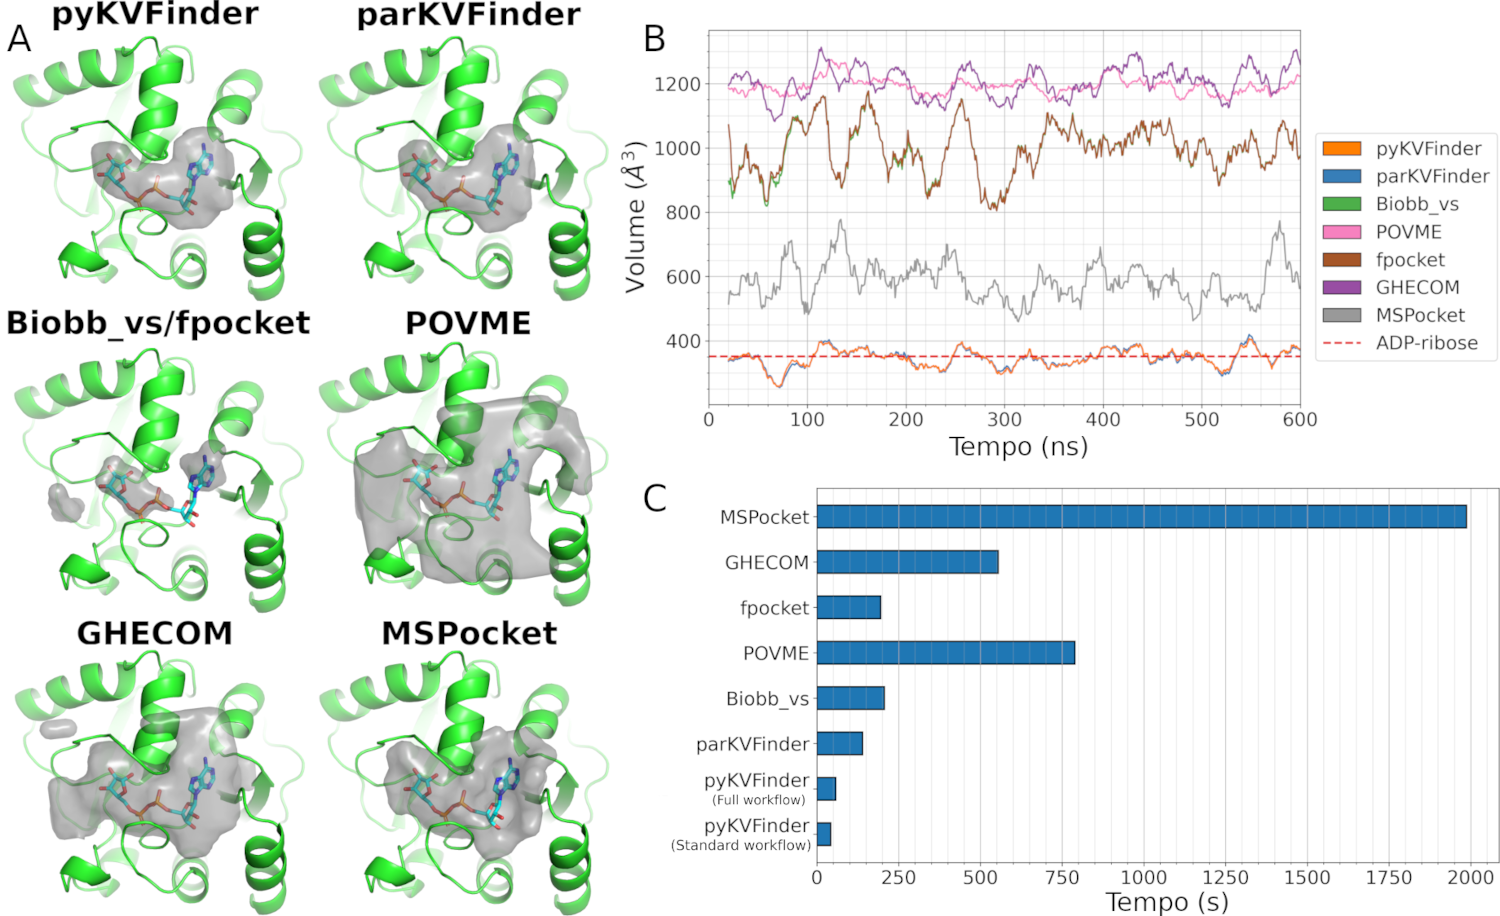
\includegraphics[scale=0.9]{images/pykvfinder-benchmarking.png}
  \centerline{\scriptsize{\textbf{Fonte:} Adaptado de \cite{guerra2021}.}}
  \caption[Avaliação de desempenho dos métodos de benchmarking para detecção do sítio de ligação do substrato da ADRP]{\textbf{Avaliação de desempenho dos métodos de benchmarking para detecção do sítio de ligação do substrato da ADRP.} \textbf{(A)} As estruturas da proteína (representadas em verde) no quadro 30 (com menor RMSD em comparação com a estrutura cristalográfica) da trajetória do domínio ADRP com as cavidades correspondentes detectadas (superfícies cinzas) por cada método de benchmarking. \textbf{(B)} O volume total das cavidades detectadas no sítio de ligação do substrato da ADRP ao longo da simulação de 600 ns. O volume total é calculado em uma janela de 20 quadros. A linha pontilhada vermelha indica o volume da superfície molecular da molécula de ADP-ribose, que ocupava originalmente o sítio de ligação do substrato da ADRP na estrutura cristalográfica (PDB ID: 6W02, cadeia B). \textbf{(C)} Tempo decorrido para detectar e caracterizar o sítio de ligação do substrato da ADRP. O protocolo padrão do pyKVFinder, assim como do parKVFinder, detecta as cavidades e aplica as caracterizações morfológicos (\eg, volume, área e forma) e topológicos (\eg, resíduos de interface e suas frequências). O protocolo completo do pyKVFinder inclui o protocolo padrão com as caracterizações de profundidade e hidropatia.}
  \label{fig:pykvfinder-benchmarking}
\end{figure}

Além de ser capaz de detectar com acurácia cavidades biomoleculares, as ferramentas atuais também devem ter um desempenho rápido na detecção e caracterização dessas cavidades. Portanto, também avaliamos o tempo decorrido para executar esses métodos de benchmarking (Figura \ref{fig:pykvfinder-benchmarking}C). O pyKVFinder superou todos os métodos analisados nesse aspecto, até mesmo ao aplicar as novas características de caracterização, profundidade e hidropatia, o tempo decorrido do pyKVFinder aumentou apenas 36\%, ainda superando os outros métodos de \textit{benchmarking}. Além disso, em comparação ao parKVFinder, o pyKVFinder foi 3,3 vezes mais rápido na detecção do sítio de ligação da ADRP. A principal razão para o ganho de desempenho é a possibilidade adicional de paralelizar rotinas, ou seja, a inserção de átomos na grade 3D na função de detecção, com base em \textit{ndarrays}. Além disso, a escalabilidade do pyKVFinder, ao aumentar o número de threads, segue o mesmo comportamento apresentado pelo parKVFinder \cite{guerra2020}. Portanto, o pyKVFinder oferece uma opção mais flexível e eficiente para usuários experientes que precisam de aplicações em larga escala, enquanto o parKVFinder é mais adequado para iniciantes devido à sua simplicidade de instalação e uso.

Para demonstrar as funcionalidades e vantagens do pyKVFinder, realizamos esse estudo em um \textit{Jupyter notebook}, onde executamos passo a passo as funções do pyKVFinder. O notebook com o caso de estudo completo está disponível em \url{https://github.com/LBC-LNBio/pyKVFinder/blob/master/examples/md-analysis/md-analysis.ipynb}. Uma descrição detalhada dessa análise está disponível no artigo publicado no periódico \textit{BMC Bioinformatics} \cite{guerra2021}.

\section{KVFinder-web \label{ap:casos-de-estudo-kvfinder-web}}

\subsection{Caracterização do sítio catalítico da protease do HIV-1}

Como exemplo ilustrativo do KVFinder-web (Figura \ref{fig:kvweb-case-study}), detectamos e caracterizamos o sítio catalítico da protease do vírus da imunodeficiência humana tipo 1 (HIV-1) ligado ao oxigênio carbonílico de ureia cíclica \cite{lam1994}, utilizando o KVFinder-web portal. Conseguimos detectar com sucesso as cavidades em toda a superfície molecular da protease do HIV-1 (Figura \ref{fig:kvweb-case-study}A). Além da detecção de cavidades e definição de sua forma, o KVFinder-web também fornece o volume, área, profundidade e hidropatia das cavidades detectadas (Figura \ref{fig:kvweb-results}B; cavidade KAG). Normalmente, o sítio ativo é a maior e mais profunda cavidade na proteína enzimática \cite{laskowski1996}, e isso também é observado na protease do HIV-1, como mostrado na Figura \ref{fig:kvweb-results}B. Nesse sentido, a caracterização da profundidade pode ajudar os pesquisadores a identificarem o sítio ativo em toda a superfície molecular. Além disso, realizamos uma análise do perfil de hidrofobicidade do sítio ativo da protease do HIV-1 (Figura \ref{fig:kvweb-case-study}C). Nossos resultados mostraram que o sítio ativo é predominantemente hidrofóbico, especialmente na região próxima aos \textbeta-hairpins, e há poucas regiões hidrofílicas ao redor dos ácidos aspárticos catalíticos (Asp-25 e Asp-25'). Conforme esperado, os subsítios S1 e S1' (região amarela) são hidrofóbicos, e os subsítios S2 e S2' são predominantemente hidrofóbicos (região amarela), exceto por Asp-29 e Asp-30 (região azul). Além disso, observamos que a parte hidrofóbica dos subsítios S2 e S2', que acomodam os substratos P2 e P2', respectivamente, tendem a favorecer cadeias laterais alifáticas \cite{lam1994,brik2002,weber2009}.

\begin{figure}[hp]
  \centering
  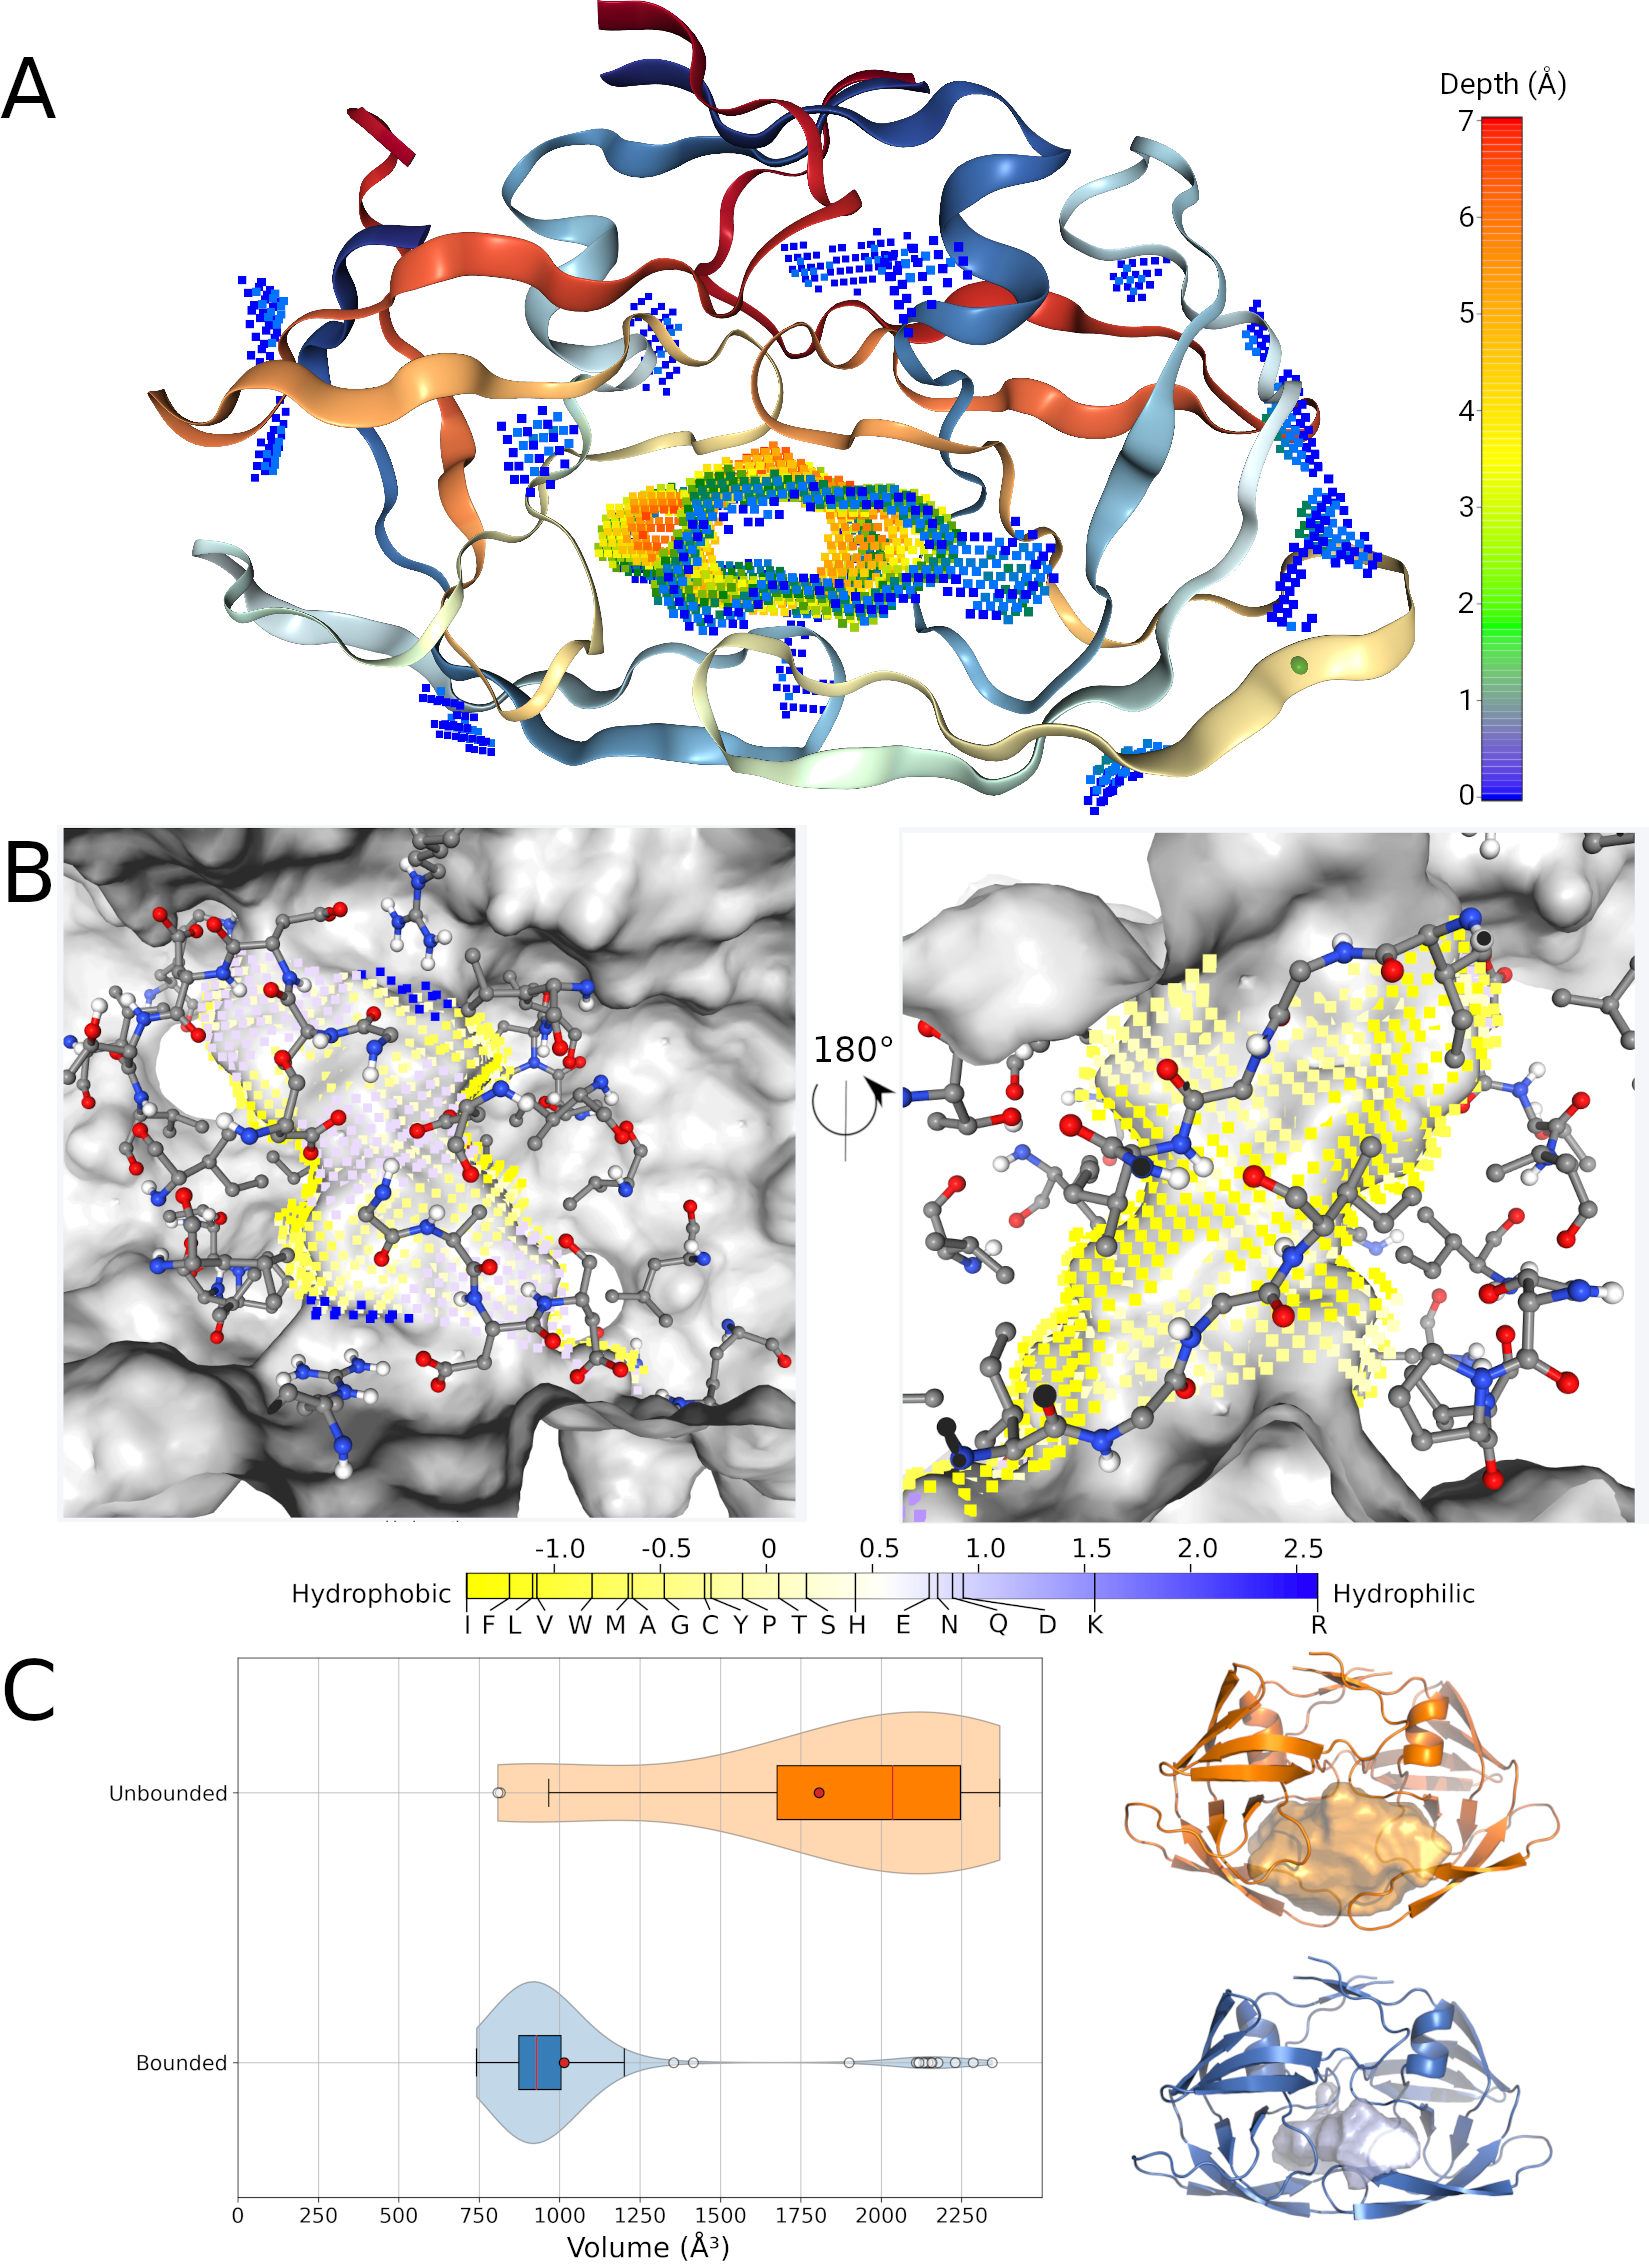
\includegraphics[scale=1.8]{images/kvweb-case-study.png}
  \centerline{\scriptsize{\textbf{Fonte:} Adaptado de \cite{guerra2023A}.}}
  \caption[Exemplo ilustrativo da detecção de cavidades na protease do HIV-1]{\textbf{Exemplo ilustrativo da detecção de cavidades na protease do HIV-1.} Estrutura molecular da protease do HIV-1 (PDB ID: 1HVR) com cavidades detectadas. \textbf{(A)} Detecção de cavidades em toda a estrutura da proteína (modelo em cartoon). Os pontos das cavidades são coloridos de acordo com a profundidade (pontos coloridos em uma escala de cores arco-íris). \textbf{(B)} Hidropatia mapeada nos pontos de cavidade na superfície nas regiões ao redor dos ácidos aspárticos catalíticos (painel esquerdo) e ao redor dos β-hairpins (painel direito). A escala de hidrofobicidade de Eisenberg & Weiss varia de -1,42 (altamente hidrofóbica) a 2,6 (altamente hidrofílica). A proteína é mostrada como uma superfície cinza e os resíduos de interface são mostrados como átomos coloridos em sticks. \textbf{(C)} Gráfico de violino do volume do sítio ativo das estruturas da protease do HIV-1 do RCSB PDB para as estruturas com ligantes ligados no sítio ativo (azul) e as estruturas sem ligantes (laranja). As estruturas com uma mediana de volume e a cavidade correspondente são mostradas como modelo em cartoon e superfície, respectivamente.}
  \label{fig:kvweb-case-study}
\end{figure}

\subsection{Comparação morfológica do sítio catalítico das estruturas da protease do HIV-1}

Conforme apresentado na Seção \ref{sec:md-hiv1-protease}, a protease do HIV-1 é um alvo terapêutico eficaz, o sítio catalítico é o alvo de diversos medicamentos antirretrovirais. No entanto, o ciclo catalítico depende dos movimentos dos \textbeta-hairpins, que controlam a acessibilidade dos substratos ao sítio ativo \cite{lam1994,soares2016}. Assim, analisamos as estruturas da protease do HIV-1 disponíveis no PDB e comparamos suas cavidades (consulte \cite{guerra2023A}). Com base nos volumes das cavidades, é possível diferenciar claramente as estruturas nas formas ligada das não-ligadas (Figura \ref{fig:kvweb-case-study}C), indicando uma complementaridade geométrica entre receptor e ligantes, juntamente com uma complementaridade físico-química, mostrada pelo perfil de hidrofobicidade discutido anteriormente.

% \section{KVFinderMD}

% \subsection{Estudo comparativo dos sítios de ligação do substrato da ALDH1 e ALDH2}

% o caso das ALDH1/2, exploramos as diferenças topológicas e volumétricas entre os sítios de ligação do substrato de ALDH1 e ALDH2, o que dita a preferência por aldeídos menores e maiores entre eles.

\chapter{Figuras suplementares \label{ap:figuras-suplementares}}

\begin{figure}[htb]
  \centering
  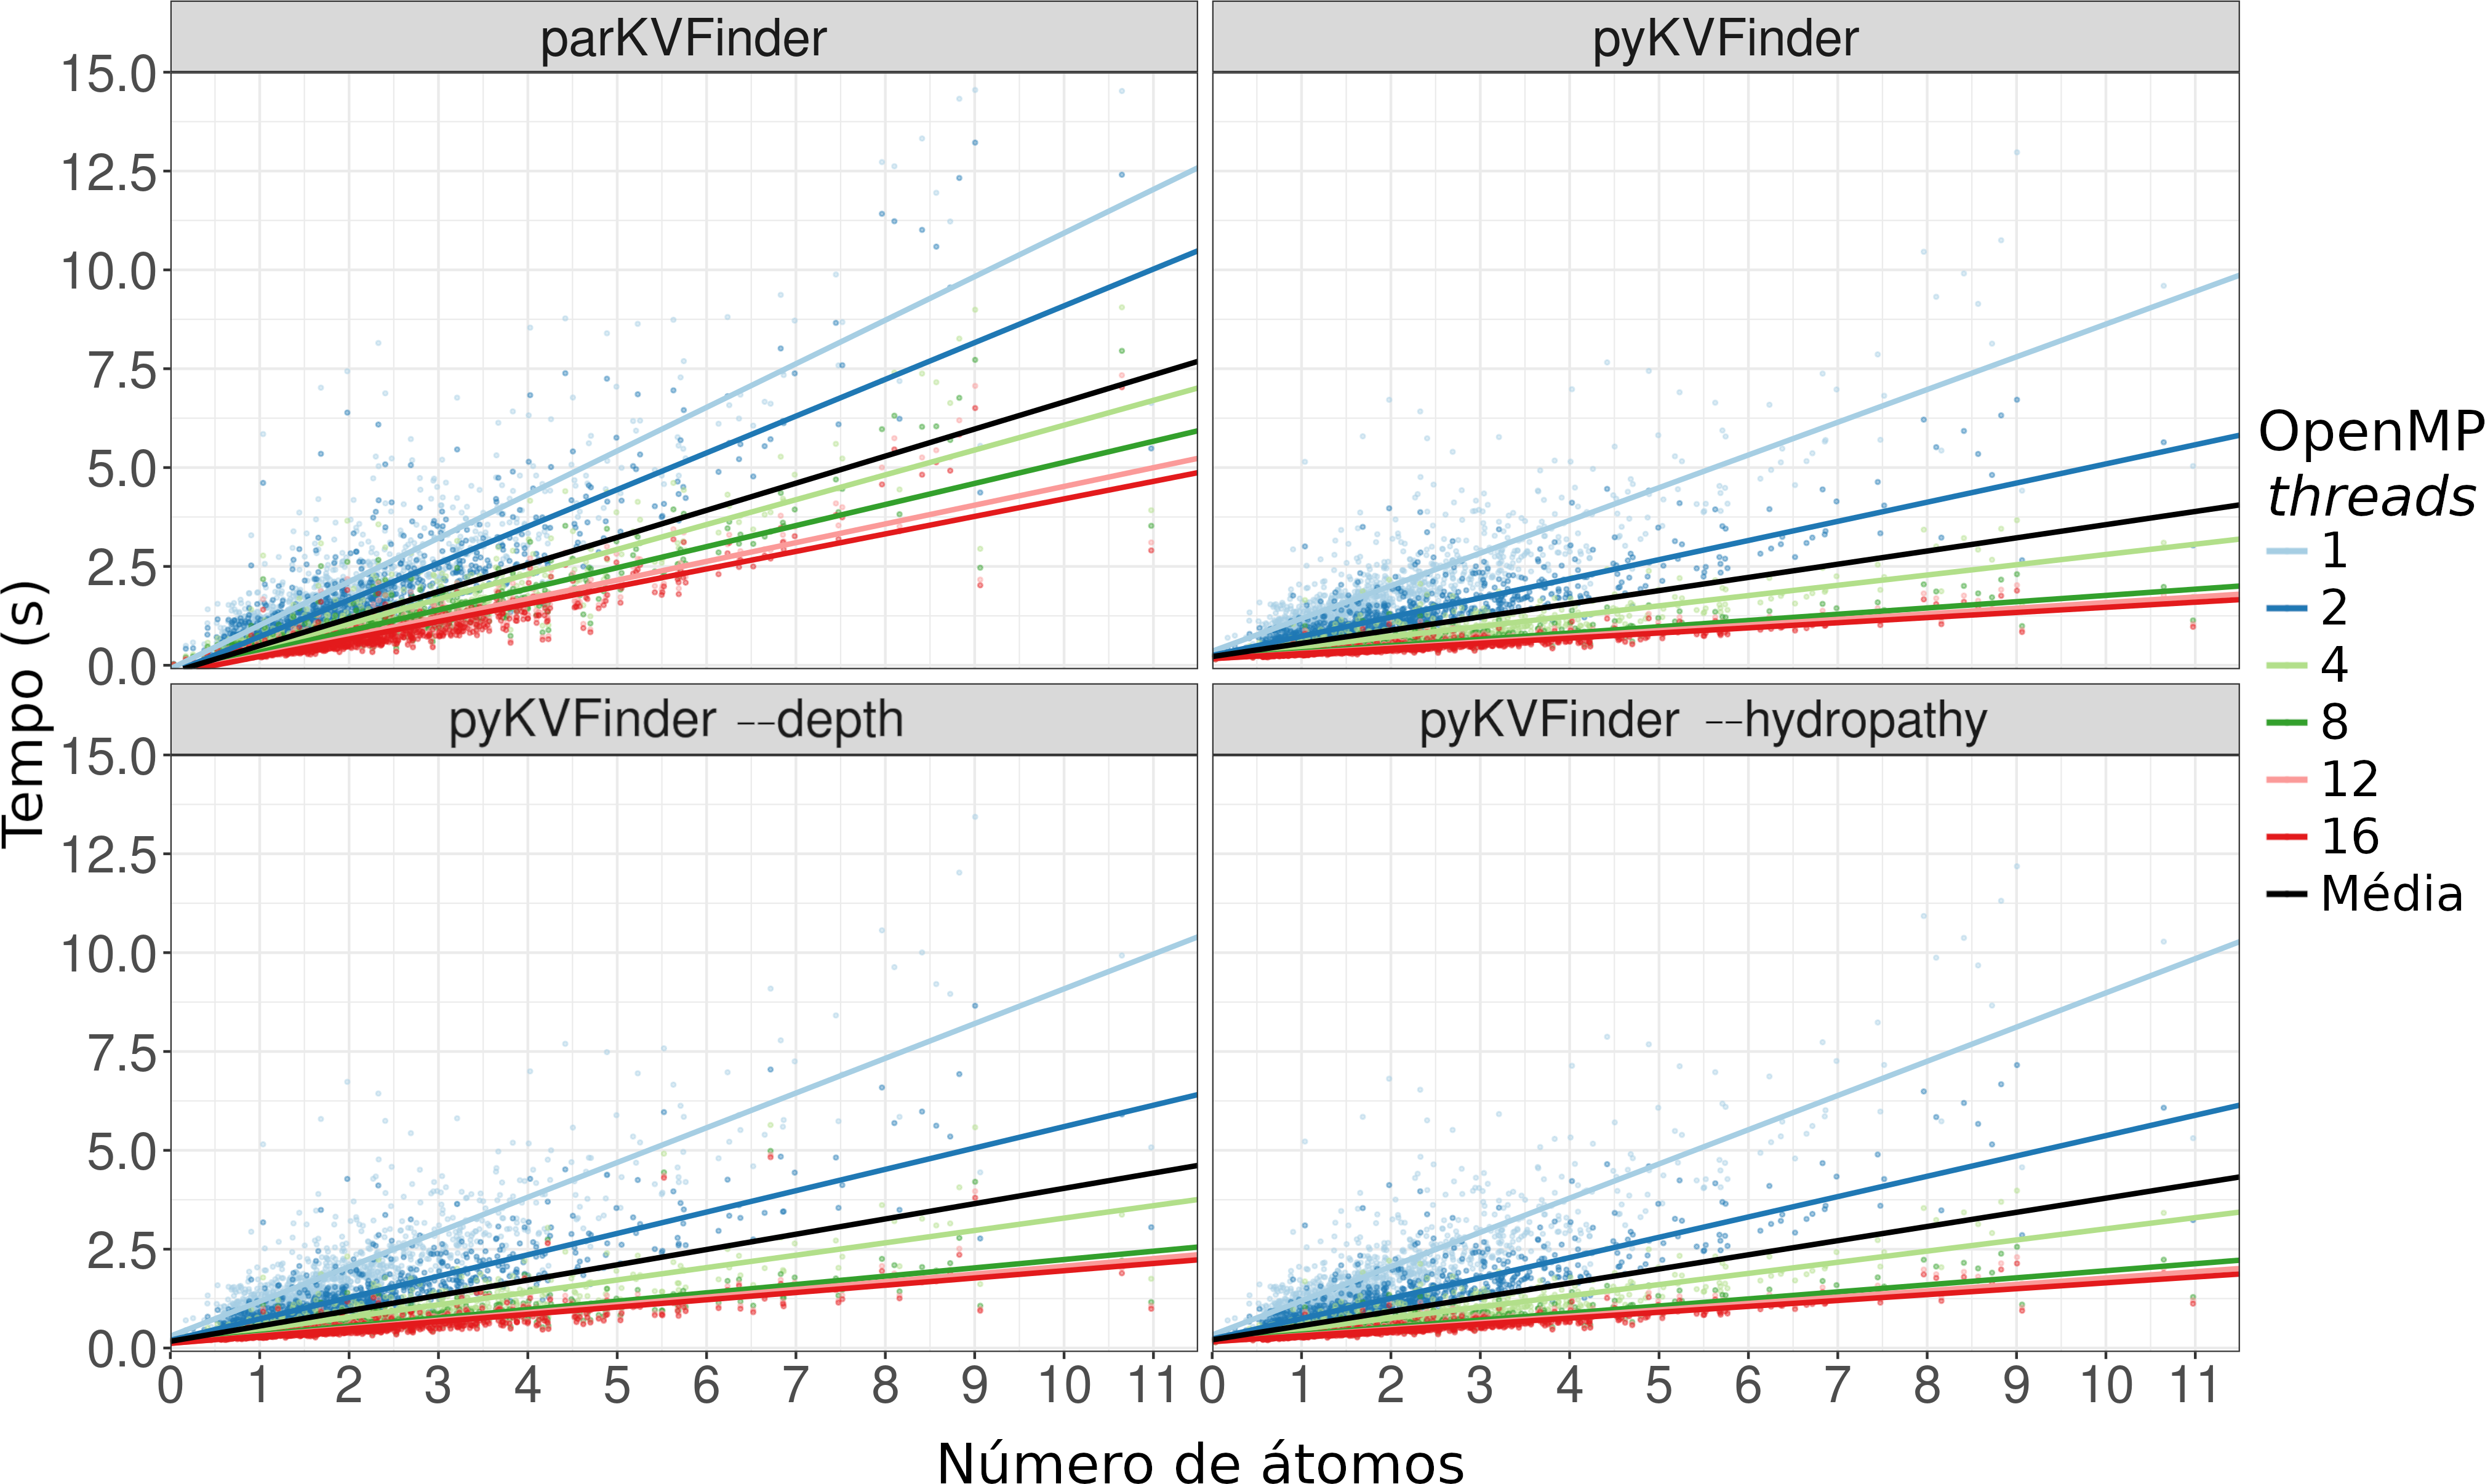
\includegraphics[scale=1]{images/pykvfinder-parkvfinder-kv1000-comparison.png}
  \caption[Tempo computacional em função do número de átomos com diferentes números de \textit{threads} para o parKVFinder e o pyKVFinder]{\textbf{Tempo computacional em função do número de átomos com diferentes números de \textit{threads} para o parKVFinder e o pyKVFinder.} Quadro superior esquerdo: parKVFinder. Quadro superior direito: pyKVFinder com caracterização padrão (volume, área e resíduos de interface). Quadro inferior esquerdo: pyKVFinder com caracterização padrão e de profundidade. Quadro inferior direito: pyKVFinder com caracterização padrão e de hidropatia}
  \label{fig:pykvfinder-parkvfinder-kv1000-comparison}
\end{figure}

\begin{figure}[htb]
  \centering
  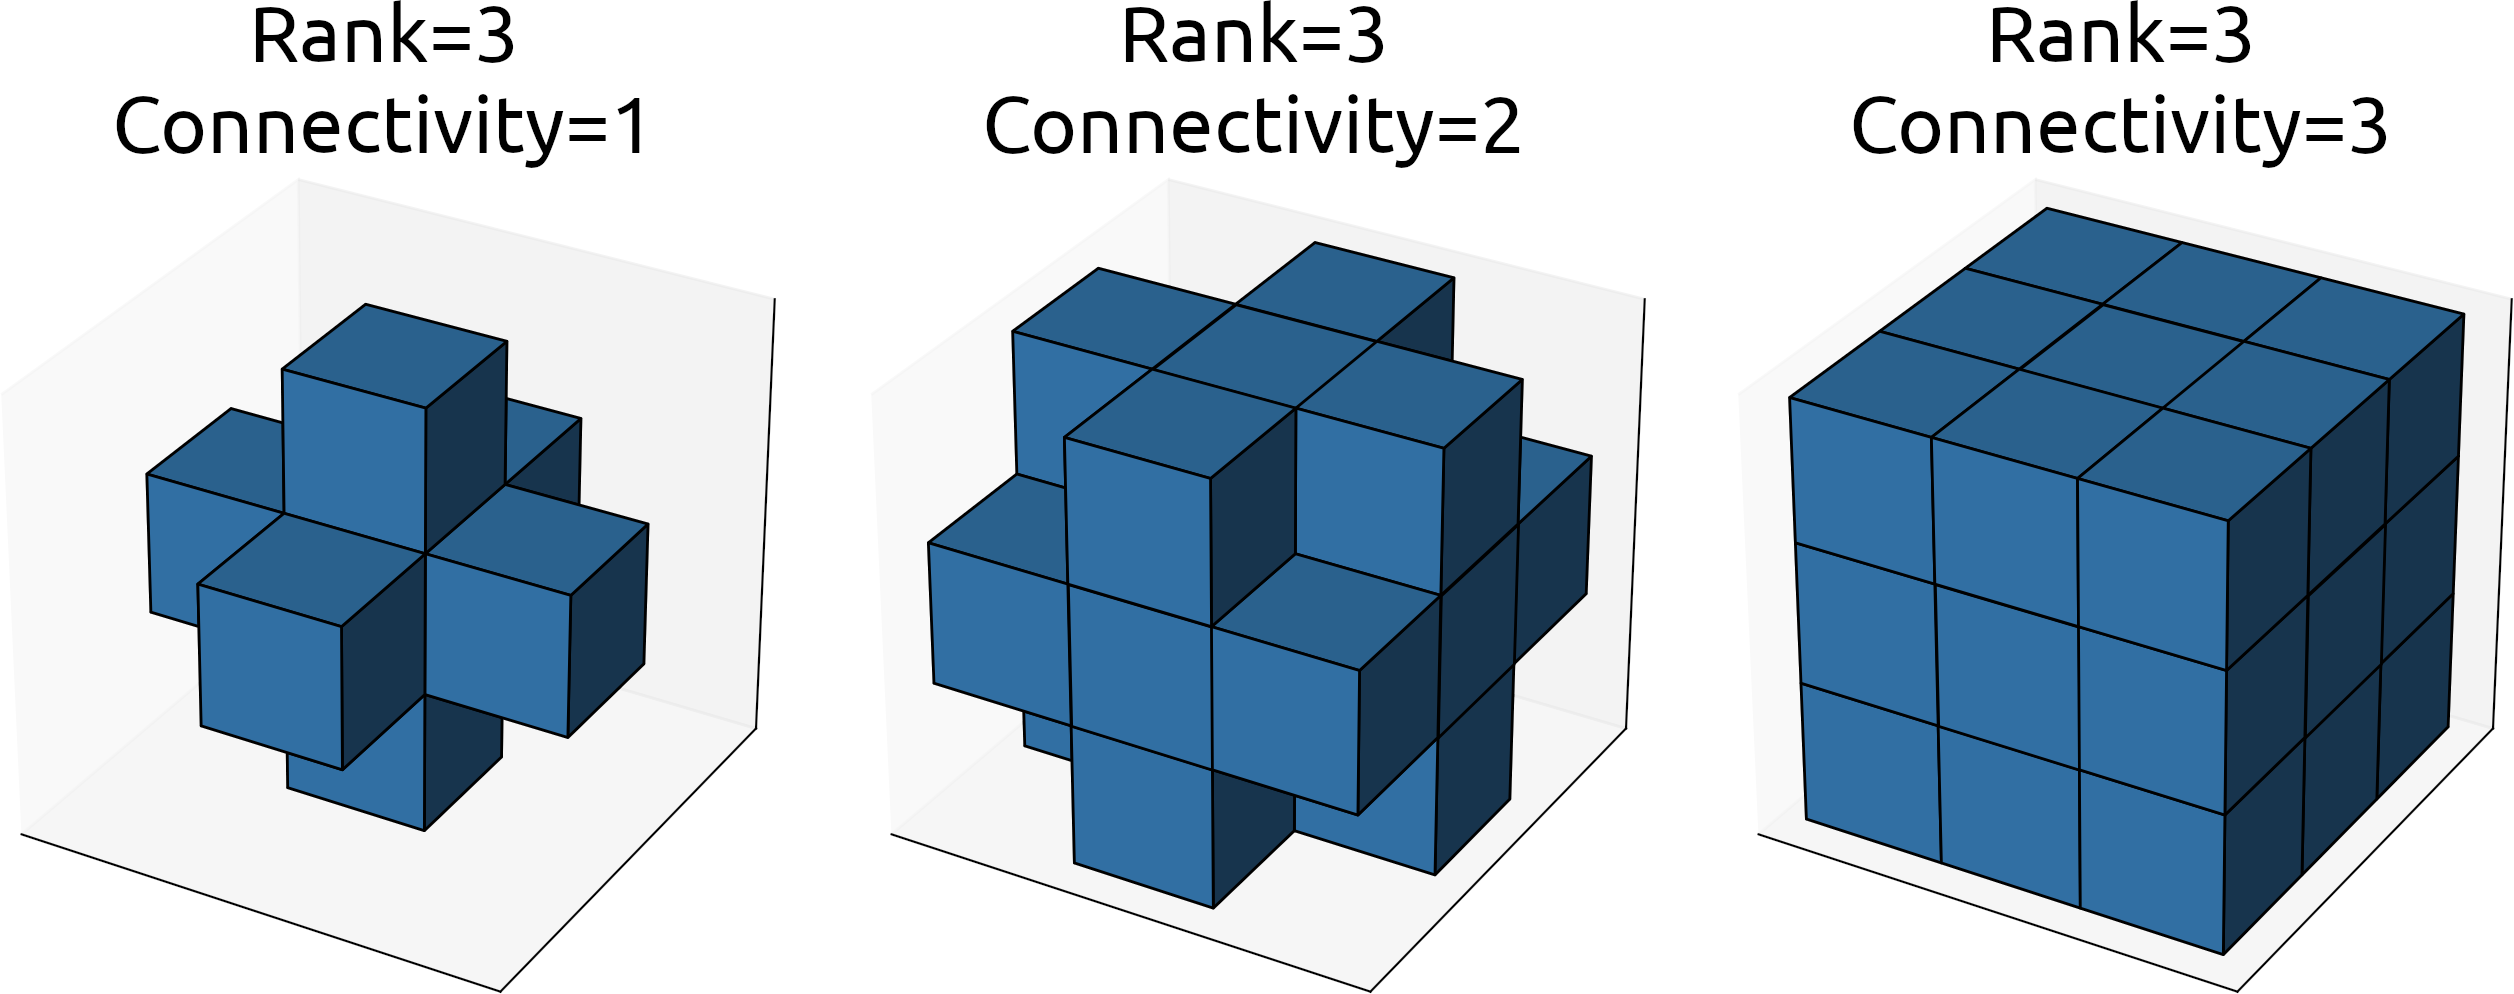
\includegraphics[scale=1]{images/3D-binary-structure.png}
  \centerline{\scriptsize{\textbf{Fonte:} Retirado de \url{https://docs.scipy.org/doc/scipy/tutorial/ndimage.html}}}
  \caption[Elementos estruturantes para filtros espaciais]{\textbf{Elementos estruturantes para filtros espaciais.}}
  \label{fig:elementos-estruturantes}
\end{figure}

\end{document}
